\documentclass[a4paper, 11pt]{report}
\usepackage[top=45mm, bottom=20mm]{geometry}
% Uni says 20cm top and bottom
% Uni says font size 12 standard.
%LEFT RIGHT ARE IN TEXT MARGIN BIT

%% Package declarations.
%\usepackage{ethesis}
\usepackage{natbib}
%\usepackage{palatino}
%\usepackage{times}
\usepackage{url}
\usepackage{setspace}
\usepackage{fancyhdr}
\usepackage{graphicx}
\usepackage{makeidx}
\usepackage{graphicx}
\usepackage{amsmath}
\usepackage{caption}

\usepackage{graphicx}
\usepackage{caption}
\usepackage{subcaption}

\usepackage{txfonts} % This seems to fix the font at the same time
\usepackage{lscape} % Allows landscape tables
\usepackage{longtable}
\usepackage{units}
\usepackage{rotating}
\usepackage{color}
\usepackage[titletoc]{appendix}
\usepackage{enumitem}

\usepackage[grey]{quotchap}

\usepackage{hyperref}
\hypersetup{colorlinks=false, pdfborder={0 0 0},}


% My definitions
\newcommand{\epsa}{\ensuremath{\varepsilon} Indi A}
\newcommand{\eps}{\ensuremath{\varepsilon} Indi}
\newcommand{\epsb}{\ensuremath{\varepsilon} Indi Ba, Bb}
\newcommand{\epsba}{\ensuremath{\varepsilon} Indi Ba}
\newcommand{\epsbb}{\ensuremath{\varepsilon} Indi Bb}
\newcommand{\micron}{\,\ensuremath{\mu}\rm{m}}
\newcommand{\mjup}{\,\ensuremath{\rm{M_{Jup}}}}

\newcommand{\magnit}{\mbox{$^{\mbox{\rm\tiny m}}$}}                   % magnitudes
\newcommand{\kmpers}{\mbox{\,km\,s$^{-1}$}}           % km s-1
\newcommand{\cmpers}{\mbox{\,cm\,s$^{-1}$}}           % cm s-1
\newcommand{\eg}{\mbox{\hbox{e.g.,}}}             % e.g. in italics
\newcommand{\etal}{\mbox{et al.}}         % et al. in italics
\newcommand{\cf}{\mbox{\hbox{\it cf.}}}               % cf. in italics
\newcommand{\idest}{\mbox{\hbox{\it i.e.}}}           % i.e. in italics

%\newcommand{\arcmin}{\mbox{.\ensuremath{\mkern-4mu^\prime}}}%    % fractional arcminute symbol: 0.'0
%\newcommand{\arcsec}{\mbox{\ensuremath{.\!\!^{\prime\prime}}}}%  % fractional arcsecond %symbol: 0.''0

%can remove these fi required
\newcommand{\arcsec}{\mbox{\ensuremath{^{\prime\prime}}}}%  % arcsecond symbol: 0''
\newcommand{\arcmin}{\mbox{\ensuremath{^{\prime}}}}%  % arcsecond 
\newcommand{\fdg}{\mbox{\ensuremath{.\!\!^\circ}}}%             % fractional degree symbol:     0.�0
\newcommand{\arcdeg}{\ensuremath{^{\circ}}}%                    % degree symbol:  �
\newcommand{\sun}{\ensuremath{\odot}}%                          % sun symbol
\newcommand{\apj}{ApJ}%                                         % Journal abbreviations
\newcommand{\apjs}{ApJS}
\newcommand{\apjl}{ApJL}
\newcommand{\aap}{A{\&}A}
\newcommand{\aaps}{A{\&}AS}
\newcommand{\mnras}{MNRAS}
\newcommand{\jrasc}{JRASC}
\newcommand{\nat}{Nature}
\newcommand{\aj}{AJ}
\newcommand{\na}{NA}
\newcommand{\araa}{ARAA}
\newcommand{\pasp}{PASP}
\def\pasa{PASA}
\newcommand{\pasj}{PASJ. \,}
\def\fcp{Fund. Cosmic Physics}
\newcommand{\Teff}{\ensuremath{T_{\mathrm{eff}}}}%              % T_eff
\newcommand{\logg}{\ensuremath{\log g}}%                        % log g
\newcommand{\bv}{\ensuremath{B\!-\!V}}%                         % B-V
\newcommand{\ub}{\ensuremath{U\!-\!B}}%                         % U-B
\newcommand{\vr}{\ensuremath{V\!-\!R}}%                         % V-R
\newcommand{\ur}{\ensuremath{U\!-\!R}}%                         % U-R
\newcommand{\asppix}{\mbox{\arcsec\,pixel$^{-1}$}}           % " pixel-1
\newcommand{\msun}{\,M$_{\ensuremath{\odot}}$}                    % " M_sun
\newcommand{\Msun}{\mbox{$M_{\mathrm{\odot}}$}}
\newcommand{\Mdot}{\mbox{$\dot M$}}
\newcommand{\Menv}{\mbox{$M_\mathrm{env}$}}
\newcommand{\Pdot}{\mbox{$\dot P$}}
\newcommand{\Tbol}{\mbox{$T_\mathrm{bol}$}}
\newcommand{\Tdust}{\mbox{$T_\mathrm{d}$}}
\newcommand{\Lbol}{\mbox{$L_\mathrm{bol}$}}
\newcommand{\Lsun}{\mbox{$L_{\odot}$}}
\newcommand{\Fco}{\mbox{$F_\mathrm{CO}$}}
\newcommand{\prob}{\hbox{P}}
\newcommand{\jh }[1]{{\bf #1}}
\newcommand{\Bin}{\mbox{\hbox{Bin}}\,}
\newcommand{\Spitzer}{{\em Spitzer}}
\newcommand{\SpitzerGB}{SGBS}
\newcommand{\SpitzerYC}{SYC}
\newcommand{\UCHII}{UCH\,\textsc{ii}}
\newcommand{\HII}{H\,\textsc{ii}}
%USE THIS COMMAND FOR TEXT, not sure this works...
\newcommand\ion[2]{#1$\;${\scshape{#2}}}%                       % ion, i.e.,CII = \ion{C}{ii}
%USE THES FOR MATHS
\newcommand\mion[2]{\mbox{#1\,{\footnotesize #2}}}      % HI properly spaced
%\newcommand{\HI}{\mbox{H\,{\footnotesize I}}}       % HI properly spaced
%\newcommand{\HII}{\mbox{H\,{\footnotesize II}}}       % HII properly spaced
%\newcommand{\CI}{\mbox{C\,{\footnotesize I}}}       % CI properly spaced
%\newcommand{\CII}{\mbox{C\,{\footnotesize II}}}       % CI properly spaced

\include{aas_macros}

%%ARP's macros:
\def\ps{$\rm km \,s^{-1}\,kpc^{-1}$}
\def\lv{\emph{l-v} }
\def\xy{\emph{x-y} }
%\def\arcdeg{$^\circ$}
\def\kms{\,km\,s$^{-1}$}
\newcommand{\sech}{\mathrm{sech} \,}
\def\H2{$\rm H_2$}
\def\torus{\textsc{torus}}
\def\phantom{\textsc{phantom}}
\def\sphng{\textsc{sphng}}
\def\Robs{$R_{\rm obs}$}
\def\Vobs{$V_{\rm obs}$}
\def\lobs{$l_{\rm obs}$}


%% Set page margins.
%% University rules: 3cm = LHS, 3cm = RHS, uni reg.
%% Top,  bottom are in geometry
% A4 is 21cm wide, 29.7cm high, uni reg, 29.7-2-2 = 25.7 text height?
\setlength{\textheight}{24cm}

%21cm - 3cm - 3cm = 15 (textwidth)
\setlength{\textwidth}{15cm}
% Latex counts margins from a 1 inch offset.
% 4cm = 1.5748 inches.
% 3cm = 1.1811 inches
\setlength{\oddsidemargin}{0.1811in}



\voffset=-1truecm

%% Set text spacing.
\onehalfspacing
%\doublespacing
%\singlespacing

%% Set paragraph indentation.
\setlength{\parindent}{30pt}


%% From eric, who got it from scw, who got it from dan price. Not sure what it does...
\pagestyle{fancy}
\fancyhead[RO,LE]{\leftmark}
\fancyfoot[C]{\thepage}
\fancyhf{}
\fancyhf[HLE,HRO]{\slshape\thepage}
\fancyhf[HLO]{\slshape\rightmark}
\fancyhf[HRE]{\slshape\leftmark}
\fancypagestyle{plain}{%
  \fancyhf{}
  \renewcommand{\headrulewidth}{0pt}
  \fancyhf[FLE,FRO]{\hfill\slshape\thepage}}

%% Tell natbib to put paper references into the index.
\citeindextrue

%% Generate the index.
\makeindex

%% Define commands to correctly include graph files from the ark. Default to
%% the bounding box for a single plot.      
%\newcommand{\graph}[2][82 80 530 670]
%{\includegraphics[angle=90, width=13cm, bb=#1]{#2}}
%\newcommand{\graphtwo}[2][20 80 567tt 680]
%{\includegraphics[angle=90, width=\columnwidth, bb=#1]{#2}}
%\newcommand{\graphthree}[2][20 110 600 720]
%{\includegraphics[angle=90, width=\columnwidth, bb=#1]{#2}}
%\newcommand{\graphfour}[2][25 73 550 695]
%{\includegraphics[angle=90, width=\columnwidth, bb=#1]{#2}}


%% Make some dotted lines for a signature and date.
\newcommand{\signed}{
   \begin{flushright}
   \begin{tabular}{rl}
   \\
   \\
   Signed: & \makebox[2in]{\dotfill}\\
           & Mr~D. J. Rumble\
   \\
   Date:   & \makebox[1.2in]{\dotfill}\\
   \end{tabular}
   \end{flushright}
}

% Copyright declaration.
\newcommand{\statement}{

   \begin{quote}\small

   Submitted by Mr Damian Rumble to the University of Exeter as a thesis for
   the degree of Doctor of Philosophy in Physics, April, 2016. 

   This thesis is available for Library use on the understanding that it is
   copyright material and that no quotation from the thesis may be published
   without proper acknowledgement. 

   I certify that all material in this thesis which is not my own work has been
   identified and that no material has previously been submitted and approved
   for the award of a degree by this or any other University.

   \end{quote}
   \signed
}
   
% Set the titlepage properties.   
\author{Damian Jack Rumble\\ \vspace{0.5in}}

%\title{{\Huge $\mathcal{S}$piral $\mathcal{P}$atterns, $\mathcal{S}$pectral $\mathcal{P}$rofiles, \\ \& $\mathcal{S}$mall $\mathcal{P}$lanets:}

%\title{{\Huge $\mathcal{T}$he $\mathcal{M}$orphology of the $\mathcal{M}$ilky $\mathcal{W}$ay}
\title{{\Huge The influence of radiative feedback on star-formation}
 \vspace{0.5in}
\\ in the James Clerk Maxwell Telescope Gould Belt Survey of nearby star-forming regions. \large \vspace{0.5in}
%\includegraphics[angle=0, width=13cm,trim=0cm 5cm 0cm 0cm]{ThesisTop}
%\\ Smaller text?
% \\ \vspace{0.5in}   PUT THIS BACK IN IF YOU REMOVE THE PICTURE.
 }
\date{\statement}

   
% Start of thesis!
\begin{document}

   % Print the titlepage.
   \maketitle
      
   % Abstract: shoudld be approximately 300 words.
  \pagenumbering{roman} % Roman numerals
  \setcounter{page}{1}
   %% Abstract.

\begin{abstract}

I aim to show that I have spent three years usefully. Or maybe four.

\end{abstract}


   % Print the contents tables.
   \tableofcontents
   \listoffigures
   \listoftables

   % Declarations where work is derived from published papers.
   %% Declaration of work previously published, and attribution.

\chapter*{}

\section*{\center Declaration}

This thesis contains work published or pending publication as papers. Honest.


   % Acknowledgements.
  %% Acknowledgements.


\chapter*{Acknowledgements}

Hey.

\vspace{0.2in} \noindent
Thanks.

\begin{flushright}
{ ME \\ Exeter, U.K. \\ ??$^{\rm th}$ September 200?}
\end{flushright}


  \pagenumbering{arabic} % Roman numerals
   % Count title page as page 1 onwards.
  \setcounter{page}{1}

   % Introductory chapter.
   %% Introduction.
% From the university regulations:
%(a) The aims, objectives and results of the candidate's research
%(b) The research methodology where not otherwise described
%(c) The contribution made by the papers in the context of the approved field
%(d) A statement of the candidate's contribution to co-authored papers
%(e) A literature review

\chapter{Introduction}
\label{ch:intro}

\section{Content (to be sorted)}

%%%MWC INTRO MATERIAL %%%%%
The temperature of gas and dust in dense, star-forming clouds is vital in determining whether or not clumps undergo collapse 
and potentially form stars \citep{Jeans:1902dz}. Dense clouds can be heated by a number of mechanisms: heating from 
the interstellar radiation field (ISRF) \citep{Mathis:1983dq, Shirley:2000uq, Shirley:2002vn}, evolved OB stars with HII regions 
\citep{Koenig:2008jo, Deharveng:2012fk} or strong stellar winds \citep{Canto:1984dq, Ziener:1999kl, Malbet:2007zr}; and 
internally through gravitational collapse of the Young Stellar Object (YSO) and accretion onto its surface \citep{calvet98}. 
%Outflows are also observed in the form of jets \citep{Skinner:1993bh, Bontemps:1996fu, Gomez:2004cr} and stellar winds 
%\citep{Drew:1997qf} as a feedback mechanism as well as radiative heating from the photosphere of the star \citep{Hatchell:2013ij}. 
Radiative feedback is thought to play an important role in the formation of the most massive stars through the suppression of 
core fragmentation \citep{Bate:2009uq, Offner:2009pt, Hennebelle:2011ly}. 
%%%MWC INTRO MATERIAL %%%%%
The temperature of star-forming regions has been observed and calculated using a variety of different methods and data. 
Some methods utilise line emission from the clouds: for example, \cite{Ladd:1994ly} and \cite{Curtis:2010zr} examine the 
CO excitation temperature and \cite{Huttemeister:1993ve} looked at a multilevel study of ammonia lines. Often temperature 
assumptions are made in line with models of Jeans instability and Bonnor-Ebert Spheres \citep{Ebert:1955vn, Bonnor:1956vn, 
Johnstone:2000fk}. An alternative method is to fit a single temperature greybody model to an observed Spectral Energy Distribution (SED) 
of dust continuum emission for the YSO \citep{Hildebrand:1983fy}; however, this method is sensitive to the completeness 
of the spectrum, the emission models and local fluctuations in dust properties \citep{Konyves:2010oq, Bontemps:2010fk}.
%%%MWC INTRO MATERIAL %%%%%
Where multiple submillimetre observations exist, low temperatures (less than 20\,K), which favour cloud collapse, can be 
inferred by the relative intensity of longer wavelengths over shorter wavelengths. For example, \emph{Herschel}  provides FIR and 
submillimetre data through PACS bands 70\,$\micron$, 100\,$\micron$ and 160\,$\micron$ and SPIRE bands 250\,$\micron$, 
350\,$\micron$ and 500\,$\micron$ \citep{Pilbratt:2010fk}. \cite{Menshchikov:2010kl, Andre:2010kx} use \emph{Herschel} 
data to construct a low resolution temperature map for the Aquila and Polaris region through fitting a greybody to dust 
continuum fluxes (an opacity-modified blackbody spectrum). \emph{Herschel} data offers five bands of FIR and submillimetre 
observations and low noise levels; however, it lacks the resolution of the JCMT which can study structure on a scale of 
7.9\arcsec (450\,$\micron$) and 13.0\arcsec (850\,$\micron$) \citep{Dempsey:2013uq} as opposed to 25.0\arcsec\ and larger 
for 350\,$\micron$ or greater submillimetre wavelengths. \cite{Sadavoy:2013qf} combine \emph{Herschel} and SCUBA-2 
data to constrain both $\beta$ and temperature.
%%%MWC INTRO MATERIAL %%%%%
This work develops a method which takes the ratio of fluxes at submillimetre wavelengths when insufficient data points exist 
to construct a complete SED. The ratio method allows the constraint of temperature or $\beta$, but not both simultaneously. 
Throughout this paper we used a fixed $\beta$. The value and justification for this are discussed in Section 3. Similar methods 
have been applied by \cite{Wood:1994qf}, \cite{Arce:1999bh} and \cite{Font:2001cr} and used by \cite{Kraemer:2003uf} 
at 12.5\,$\micron$ and 20.6\,$\micron$ and by \cite{Schnee:2005zr} at 60\,$\micron$ and 100\,$\micron$. \cite{Mitchell:2001ve} 
first used 450\,$\micron$ and 850\,$\micron$ fluxes from SCUBA, though full analysis was limited by the quality and quantity of 
450\,$\micron$ data. A more rigorous analysis of SCUBA data was completed by \cite{Reid:2005ly} who are able to constrain 
errors on the temperature maps from sky opacity and the error beam components. Most recently similar methods have 
been used by \cite{Hatchell:2013ij} to analyse heating in NGC1333. This work looks to utilise these methods to further 
investigate radiative feedback in star-forming regions. 

\section{Radiative Transfer Theory}
\subsection{Dust}
\subsection{Dust models/assumptions - opacity}
\subsection{Jayliegh Jeans limit}

\section{Protostars}
\subsection{Jeans mass/stability}
\subsection{SED models}
\subsection{Classification: Alpha}
\subsection{Classification: Bolometeric Luminosity}
\subsection{Classification: Bolometeric temperature}
\subsection{Classification: Colour diagrams}
\subsection{Evolution/timescale: MvsL diagrams}
\subsection{IMF/CMFs}

\section{Radiative feedback}
\subsection{OB stars}
\subsection{Winds}
\subsection{RDI}
\subsection{HII regions}
\subsection{Jets}
\subsection{Radiative heating by OB stars}

\section{Accretion}
\subsection{Discs}
\subsection{Envelopes}

\section{Emission}
\subsection{IR}
\subsection{Submm}
\subsection{Radio}
\subsection{X-ray}

\section{Properties}
\subsection{Flux/photometery}
\subsection{Mass}
\subsection{Column density}
\subsection{Volume density}
\subsection{Proper motion}
\subsection{Extinction}

\section{Molecular Line emission}
\subsection{CO}
\subsection{Masers}
\subsection{Other}

\section{Triggered/none triggered star formation?}

 

   % The JCMT Gould Belt Survey of star forming regions
   \chapter{The JCMT Gould Belt Survey of star forming regions}
\label{ch:chapter2}

\section{Observational astronomy}
\subsection{Observing in submillimetre}
\subsection{SCUBA-2}

Our work builds on analytical techniques developed for SCUBA data \citep{Johnstone:2000fk, Kirk:2006vn, Sadavoy:2010ve} 
to analyse SCUBA-2 data at the same wavelengths. SCUBA-2 represents a significant improvement over 
its predecessor as it has an array of 10,000 pixels, as opposed to 128. Practically this gives the instrument a 
much wider field of view and allows larger regions to be observed quicker and to greater depth. Restricted 
to SCUBA, larger regions of star formation, for example Orion \citep{Nutter:2007ys} and Perseus 
\citep{Hatchell:2007qf}, were prioritised over the low mass Serpens MWC 297 region.

The JCMT GBS extends the coverage of the local star-forming regions over those mapped by SCUBA. SCUBA-2 
also offers much greater quality and quantity of 450\,$\micron$ data, as a result of improved array technology and 
reduction techniques pioneered by \cite{Holland:2006uq, Holland:2013fk}, \cite{Dempsey:2013uq} and 
\cite{Chapin:2013vn}. \cite{Mitchell:2001ve} is able to construct partial temperature maps from SCUBA 450\,$\micron$ 
and 850\,$\micron$ data but is limited to general statements about the region as a result of high noise estimates at 
450\,$\micron$. \cite{Reid:2005ly} go further in their use of 450\,$\micron$ data to analyse clump temperature but 
only obtain results for 54\,per cent of the clumps they detect in 850\,$\micron$. Calculated temperatures become 
increasingly unreliable at higher values to the extent they can only define a lower limit of 30\,K for temperatures 
above this value. 

%This survey is deeper than most SCUBA studies, this is demonstrated through an order of magnitude improvement in completeness with one out every three clumps we detect being the below the completeness limit of 0.4 $M_\odot$ specified by \cite{Johnstone:2000fk}.

The lower noise levels and wider coverage at 450\,$\micron$ from SCUBA-2 offer improved quality and 
quantity to the extent that temperature maps can be constructed for many features in star-forming regions.

\subsection{Data reduction}
%FROM MWC 297
The data were reduced using an iterative map-making technique (\texttt{makemap} 
in {\sc smurf}, \citeauthor{Chapin:2013vn} \citeyear{Chapin:2013vn}, 
\citeauthor{Jenness:2013fk} \citeyear{Jenness:2013fk}), and gridded to 6\arcsec\ 
pixels at 850\,$\micron$, 4\arcsec\ pixels at 450\,$\micron$.  
The iterations were halted when the map pixels, on average, changed by 
$<$0.1\,per cent of the estimated map rms. The initial reductions of each individual 
scan were coadded to form a mosaic from which a signal-to-noise mask was 
produced for each region.  This was combined with \emph{Herschel} 500\,$\micron$ 
emission at greater than 2\,Jy/beam to include all potential emission regions. 
The final mosaic was produced from a second reduction using this mask to define 
areas of emission. Detection of emission structure and calibration accuracy
are robust within the masked regions, and are uncertain outside of the masked 
region. %The reduced map and mask are shown in Figure \ref{fig:maps}.
%FROM MWC 297
A spatial filter of 600\arcsec\ is used in the reduction, which means that flux 
recovery is robust for sources with a Gaussian Full Width Half Maximum (FWHM) 
less than 2.5\arcmin. Sources between 2.5\arcmin\ and 7.5\arcmin\ will be 
detected, but both the flux and the size are underestimated because Fourier 
components with scales greater than 5\arcmin\ are removed by the filtering 
process. Detection of sources larger than 7.5\arcmin\ is dependent on the 
mask used for reduction.
%FROM MWC 297
The data presented in Figure~\ref{fig:maps} are initially calibrated in units of pW 
and are converted to Jy per pixel using Flux Conversion Factors (FCFs) derived 
by \cite{Dempsey:2013uq} from the average values of JCMT calibrators. 
By correcting for the pixel area, it is possible to convert maps of units Jy/pixel 
to Jy/beam using 
\begin{equation}
S_{\textup{beam}} = S_{\textup{pixel}}\frac{\textup{FCF}_{\textup{peak}}}{\textup{FCF}_{\textup{arcsec}}}\frac{1}{\textup{Pixel area}}.
\label{eqn:pixelFCF} 
\end{equation}
%\begin{equation}
%S_{\textup{pixel}} = S_{\textup{beam}}\frac{\textup{Pixel area}}{\textup{Beam area}}
%\label{eqn:pixelgen} 
%\end{equation}
%FROM MWC 297
FCF$_{\mathrm{arcsec}}$ = 2.34$\pm$0.08 and 4.71$\pm$0.5 Jy/pW/arcsec$^{2}$, 
at 850\,$\micron$ and 450\,$\micron$ respectively, and FCF$_{\mathrm{peak}}$ = 537$\pm$26 
and 491$\pm$67 Jy/pW at 850\,$\micron$ and 450\,$\micron$ respectively. The PONG 
scan pattern leads to lower noise in the map centre and overlap regions, while data 
reduction and emission artefacts can lead to small variations in the noise over the whole 
map. 

\subsection{Calibration}
\subsection{Related surveys - 2MASS/Spitzer/Herschel}

%5.8\arcsec (70\,$\micron$), 7.1\arcsec (100\,$\micron$), 11.2\arcsec (160\,$\micron$), 18.2\arcsec (250\,$\micron$), 25.0\arcsec (350\,$\micron$) and 36.4\arcsec (500\,$\micron$) with \emph{Herschel} \citep{Aniano:2011fk}. 

\section{Data enhancement}
\subsection{Selection}
%FROM MWC 297
\begin{figure*}[t!]
\begin{centering}
\includegraphics[scale=0.35]{/Users/damian/Documents/Thesis_et_al/images/20130912_rms_tau_450.pdf}\includegraphics[scale=0.35]{/Users/damian/Documents/Thesis_et_al/images/20130912_rms_tau_850.pdf}
\caption{Plots of optical depth due to water vapour, tau, as a function of noise level of the data in the 6 component scans of MWC 297 at 450\,$\micron$  \emph{(left)} and 850\,$\micron$ \emph{(right)}. Tau is measured at two frequencies, 225GHz  \emph{(red)} and 186GHz \emph{(blue)}. Note how the majority of points are on linear trend (within measured errors), with the exception of one scan 450$\microns$ which was subsequently rejected from the final mosaic.} \label{fig:tau}
\end{centering}
\end{figure*} 
%FROM MWC 297
Of the six scans observed, three were selected for the final mosiac at each wavelength. This selection reflects a number of factors. In one case observed flaws were attributed to bolometer failures in one 850\,$\micron$ case and weather conditions where the opacity was significantly off trend in both $\tau_{225}$ and $\tau_{186}$ bands for a 450\,$\micron$ case (Figure~\ref{fig:tau}). Both scans were removed. 
%FROM MWC 297
A perceived `temperature gradient' remained in the preliminary results and was unexplained by contemporary understanding of star formation. We devised a test for reliability of the data, comparing a pixel in one scan to the mean of the remaining five. Where this pixel was greater than three standard deviations from the mean it was flagged as `anomalous'. Typical fraction of anomalies due to statistical noise within the data reduction masks of MWC 297 region were $~3per cent$ and $~6per cent$ for 450\,$\micron$ and 850\,$\micron$. Two out of five scans were rejected from 450\,$\micron$ with fractions of $7per cent$ and $10per cent$ and two out of five scans were rejected from 850\,$\micron$ with fractions of $17per cent$ and $50per cent$. 
%FROM MWC 297
The omission of half of the components has a none negligible effect on the background $1\sigma$ noise level of the maps, causing it to increase from $16.8$/$2.18$ to $20.9$/$2.62$ mJy per 4\arcsec\ /6\arcsec\  pixel, 450\,$\micron$/850\,$\micron$ respectively. 

\subsection{Mosiacs}
\subsection{Filtering}
\subsection{Clumpfinding}
\subsection{FINDBACK}
\subsection{FELLWALKER}

%A simplified approach to a `clump' in the ISM models it as a sphere of gas with a Gaussian-like density profile. It is not feasible to constrain a real radius of the volume of this clumps and instead we turn to an artificial, \emph{effective radius}. The effective radius is smaller than reality as it measures from the centre of the clump to where the density profile drops below the noise level as opposed to where the density becomes indistinguishable from the ISM. The inevitable consequence of a smaller clump radius is a smaller integrated flux for the clump. Whilst effective radius does not provide a real measure of clamp mass, it does provide a mechanism for defining a lower limit on the mass of the clump by defining a minimum clump size. 

Clumps do not have well defined boundaries within the ISM. We use the signal to noise 
ratio to define a boundary at an \emph{effective radius}. The boundary is determined 
by the \textsc{starlink} \textsc{CUPID} package for the detection and analysis of objects 
\citep{Berry:2013uq}, specifically the \textsc{fellwalker} algorithm which assigns pixels to 
a given region based on positive gradient towards a common emission peak. This method 
has greater consistency over parameter space than other algorithms (Watson 
\citeyear{watson:2010pc}, \cite{Berry:2014vn}). \textsc{fellwalker} was developed by 
\cite{Berry:2007vn}, and the 2D version of the algorithm used here considers a pixel in the data 
above the noise level parameter and then compares its value to the adjacent pixels. \textsc{fellwalker} then moves on to 
the adjacent pixel which provides the greatest positive gradient. This process continues 
until the peak is reached - when this happens all the pixels in the `route' are assigned 
an index and the algorithm is repeated with a new pixel. All `routes' that reach the same 
peak are assigned the same index and form the `clump'.  Clump-finding algorithms, 
such as this, have been used by \cite{Johnstone:2000fk}, \cite{Hatchell:2005fk}, \cite{Kirk:2006vn} 
and \cite{Hatchell:2007qf} to define the extent of clumps for the purposes of measuring 
clump mass. 

%A simplified approach to a `clump' in the ISM models it as a sphere of gas with a Gaussian-like density profile. In this scenario a radius would exist where the density of the clump becomes indistinguishable from a constant density ISM and this forms the basis for the calculation of Jeans masses and lengths. Ideally this radius could be used to define an area from which the total flux could be observed and subsequently be used to calculate mass of the clump. Observations of clumps show they are rarely spherical or any regular volume. Density profile varies depending on how evolved the clumps and whether it has started collapsing to form a protostar or not and the ISM is not constant level. In addition to these problems, observational data comes with a maximum level of statistical noise in the flux, under which uncertainty is too high for reliable data. 


\section{Statistical noise}
\subsection{Methods}
\section{GBS regions}

%family portrait
\begin{figure*}[t!]
\begin{centering}
\includegraphics[scale=0.7]{images/map_aquila_rift_B10.pdf}
\caption{A visual extinction map of the whole Serpens/Aquila region derived from 2MASS data. Of particular interest are the Serpens Main and W40/Serpens South region. Note that whilst these two last regions appears as one continuous feature on this map, they are thought to be separate features (labeled respectively with the circle and star). The dashed rectangle indicates an area examined by Herschel and discussed by \cite{Bontemps:2010fk} } \label{fig:11}
\end{centering}
\end{figure*} 

%FROM MWC 297
This study uses data from the JCMT Gould Belt Survey (GBS) of nearby star-forming regions \citep{WardThompson:2007ve}. 
The survey maps all major low and intermediate-mass star-forming regions within 0.5 kpc. The JCMT GBS provides some of the 
deepest maps of star forming regions where $A_v > 3$  with a target sensitivity of 3 mJy beam$^{-1}$ at 850\,$\micron$ and 12 mJy 
beam$^{-1}$ at 450\,$\micron$. The improved resolution of the JCMT also allows for more detailed study of large scale 
structures such as filaments, protostellar envelopes, extended cloud structure and morphology down to the Jeans length.

In this section, the basic properties of each region are presented and studies at a variety of wavelengths are discussed to highlight the diversity of astrophysics in the Aquila-rift. This is an elongated region of extinction at $l~=~28^{\circ}$. Studies by \cite{Straizys:2003nx} have calculated a distance of 225 $\pm$ 55 pc for the `extinction wall' of the region. The rift itself is a vast dust feature spanning approximately $5\,^{\circ}$ in length and is clearly visible in figure \ref{fig:11} \citep{Bontemps:2010fk}. 

Serpens Main, Ammonia and South are vast, complex systems with filaments and well defined core regions within the clouds. Star formation here is thought to have started from the spontaneous collapse of the molecular clouds under gravity - hereby referred to as \emph{`classical'} star formation. It is fairly ubiquitous that these regions with contain a core region of the most dense, cold gas with filaments off shoots. These regions are grouped such that they do not feature isolated collapse or obvious previous generations of stars that may be influencing the environment from which they are formed, for example with a Photo-Dissociative region (PDR).

W40, MWC297 and VV Ser regions of Serpens-Aquila are smaller and fundamentally different to the classical star forming regions. That is to say each region is synonymous with some existing MS stars which have recently formed from the natal cloud and are thought to be in someway influencing star formation in the region. MWC297 and VV Ser contain isolated, young MS or Zero Age Main Sequence (ZAMS) stars. W40 contains a developed OB association of 3 ionising stars which are responsible for a large DPR. Together they are designated as potentially \emph{`triggered'} star forming regions.

The rift is the common cloud that Serpens Main, Ammonia and VV Ser are all part of, therefore the distance of 225$\pm$55pc is carried through for the distance to Serpens South as the regions are physically connected, Figure \ref{fig:serpensIR} shows the regions in relation to each other. In addition to this, South also has similar Local Standard of Rest velocity (~6$km^{-1}$) as Main and $NH_3$ \citep{Gutermuth:2008fk}.  Observations of Serpens South are complicated by the presence of W40 which is projected on the same part of the sky as South. There has been considerable debate over its distance of W40 relative to South. From this point on it is assumed that W40 is at a distance of ~600pc and is therefor not physically connected to South. 

Finally, other notable regions of Serpens-Aquila are discussed, namely this is a poorly studied Eastern region. [EXPAND AND INCLUDE N]

I summarise the regions here. 

\begin{itemize}
\item \textbf{Serpens Main} is located approximately \emph{$\alpha$: 18 29 55 $\delta$: +01 13 00} (Galactic coordinates is l = $32\,^{\circ}$ and b = $5\,^{\circ}$) at a distance of $230\pm20$ps \citep{Eiroa:2008ta} with an approximate depth of 80 pc. 
\item \textbf{Serpens Ammonia} (from now on $NH_3$) is located 45' to the south of Serpens Main \citep{Djupvik:2006fk} and is undergoing many similar star formation processes to its `sister' region to the north. 
\item \textbf{Serpens South} is one half of the Aquila-Rift Molecular cloud complex located at  approximately \emph{$\alpha$:18 30 03, $\delta$:-02 01 58.2}  (l = $28\,^{\circ}$ and b = $5\,^{\circ}$). It is located approximately $3\,^{\circ}$ south of the previous discuss Serpens Main region.
\item \textbf{W40} is coincident with Serpens South and is composed of three components; a large cold molecular cloud, a powerful HII region (S2-64) driven by a three star OB association and a embedded stellar cluster. 
\item \textbf{Serpens MWC 297} is an important, isolated intermediate mass ZAMS star to the south east of W40 at  \emph{$\alpha$: 18 27 40.6 $\delta$: -03 50 11}.
%\item \textbf{VV Serpens} is a young UX Variable Orion Star located at \emph{$\alpha$: 18 28 48 $\delta$: +00 08 40} roughly 20' to the south of Serpens $NH_3$.
\item \textbf{Serpens East} is the most prominent of several smaller eastern regions located approximately \emph{$\alpha$: 18 37 30 $\delta$: -01 40 00}.
\item \textbf{Serpens North} is the most prominent of several smaller eastern regions located approximately \emph{$\alpha$: 18 37 30 $\delta$: -01 40 00}.
\end{itemize}

Spatial distribution has been analysed by various authors for various regions through the means of a quantifiable ratio between the number of PMS to protostars in a given part of the cloud, for example, the core. Here I conduct a similar analysis, the results of which are shown in Table \ref{table:ratio}. Ratios are calculated for the entire map as a control and then for two different sized cores. These areas are shown on the YSO maps for each region above as the blue dotted and solid lines. Each area is defined by an arbitrary flux level such that a sensible core region is defined. There is a mixed bag of results to compare this directly to as some areas have been studied in this fashion whereas others have not and there are few limits places on the boundary conditions. The results obtained here will be discussed relative to the literature results in the discussion section with the main focus being on trends as opposed to actual data. 

\begin{table}[ht]
\centering
\begin{tabular}{l | p{1cm} p{1cm}  p{1cm}  p{1cm}  p{1cm}  }
	Region	&	Whole map	&	0.03Jy per beam	&	0.1Jy per beam 	&	0.25Jy per beam	&	0.3Jy per beam\\
	\hline
	Main		&	0.26			&	-			&	0.92			&	1.62			&	-		\\
	$NH_3$	&	0.13			&	-			&	1.13			&	7.00			&	-		\\	
	South	&				&	5.70			&	-			&	-			&	19.00	\\
	MWC297	&	0.10			&	-			&	n/a			&	0.40			&	-		\\
\end{tabular}
\caption{Results of analysis of ratio of protostars to pre-main sequence stars for the whole maps and the core region, defined by an arbitrary flux level. [UPDATE]}
\label{table:ratio}
\end{table}


%FROM MWC 297
\subsection{Serpens MWC 297}

\begin{figure*}
\begin{centering}
\includegraphics[scale=0.7]{/Users/damian/Documents/Thesis_et_al/images/20140718_MWC297_s450+s850_final.pdf}
\caption{SCUBA-2 450\,$\micron$ (\emph{left}) and 850\,$\micron$ (\emph{right}) data. Contours show 5$\sigma$ and 15$\sigma$ levels in both cases: levels are at 0.082, 0.25 Jy/ 4\arcsec\ pixel and 0.011, 0.033 Jy/ 6\arcsec\ pixel  at 450\,\micron\ and 850\,\micron\ respectively. The blue outer contour shows the data reduction mask for the region, based on \emph{Herschel} 500\,$\micron$ observations. Noise levels increase towards the edges of the map on account of the mapping method outlined in Section 2.1.} \label{fig:maps}
\end{centering}
\end{figure*} 

Serpens MWC 297 region is a region of low mass star formation associated with the B star MWC 297 and 
considered to be part of the larger Serpens-Aquila star forming complex (Figure \ref{fig:maps}). 

%FROM MWC 297
Serpens MWC 297 was observed with SCUBA-2 \citep{Holland:2013fk} on the 5th and 
8th of July 2012 as part of the JCMT Gould Belt Survey (GBS, \citeauthor{WardThompson:2007ve} 
\citeyear{WardThompson:2007ve}) MJLSG33 SCUBA-2 Serpens Campaign 
\citep{Holland:2013fk}. One scan was taken on the 5th at 12:55 UT in good 
Band 2 with 225 GHz opacity $\tau_{\mathrm{225}} = 0.04-0.06$. Five further scans 
taken on the 8th between 07:23 and 11:31 UT in poor Band 2, $\tau_{\mathrm{225}} 
= 0.07-0.11$.
%FROM MWC 297
Continuum observations at 850\,$\micron$ and 450\,$\micron$ were made using 
fully sampled 30\arcmin\ diameter circular regions (PONG1800 mapping mode, 
\citeauthor{Chapin:2013vn} \citeyear{Chapin:2013vn}) centered on RA(J2000) = 
$18^{h}$ $28^{m}$ $13^{s}.8$, Dec. (J2000) = $-03^{\circ}$ $44'$ 1.7\arcsec.
%FROM MWC 297
Typical noise levels were 0.0165 and 0.0022 Jy per pixel at 450\,$\micron$ and 
850\,$\micron$ respectively.

The exact distance to the star MWC 297 is a matter of debate. Preliminary 
estimates of the distance to the star were put at $450\hbox{ pc}$ by \cite{Canto:1984dq} and $530\pm70\hbox{ pc}$ 
by \cite{Bergner:1988bh}. \cite{Drew:1997qf} used a revised spectral class of B1.5Ve to calculate a closer distance of 
$250 \pm 50\hbox{ pc}$ which is in line with the value of $225\pm55\hbox{ pc}$ derived by \cite{Straizys:2003nx} for 
the minimum distance to the extinction wall of the whole Serpens-Aquila rift of which the star MWC 297 is thought to be a part. 
The distance to the Serpens-Aquila rift was originally put at a distance of $250 \pm 50\hbox{ pc}$ due to association with 
Serpens Main, a well constrained star forming region the north of MWC 297; however, recent work by \cite{Dzib:2010dq,Dzib:2011cr} 
has placed Serpens Main at $429\pm2 \hbox{ pc}$ using parallax. \cite{Maury:2011ys} argues that previous methods measured 
the foreground part of the rift and that Serpens Main is part of a separate star forming region positioned further back. 
On this basis, we adopt a distance of $d = 250\pm50\hbox{ pc}$ to the Aquila rift and the Serpens MWC 297 region \citep{Sandell:2011dz}. 

%FROM MWC 297
The star MWC 297 is an isolated, intermediate mass Zero Age Main Sequence (ZAMS) star located to the south east of Serpens South at RA(J2000) = $18^{h}$ 
$27^{m}$ $40^{s}.6$, Dec. (J2000) = $-03^{\circ}$ $50'$ 11\arcsec. \cite{Drew:1997qf} noted that MWC 297 has strong reddening 
due to foreground extinction ($A_V$ = 8) and particularly strong Balmer line emission. The star has been much studied as an 
example of a classic Herbig AeBe star, defined by \cite{Herbig:1960eu}, \cite{Hillenbrand:1992kl} and \cite{Mannings:1994kx} 
as an intermediate mass (1.5 to 10\,$M_{\odot}$) equivalent of classical T-Tauri star, typically a Class III pre-main sequence 
star of spectral type A or B. 

%FROM MWC 297
Herbig AeBe stars are strongly associated with circumstellar gas and dust with a wide range of temperatures. \cite{Berrilli:1992cr} 
and \cite{di-Francesco:1994dq,  di-Francesco:1998fk} find evidence of an extended disk/circumstellar envelope around the star MWC 297. 
Radio observations constrain disk size to $< 100$\,AU and also find evidence for free-free emission at the poles that suggest the 
presence of polar winds or jets \citep{Skinner:1993bh, Malbet:2007zr, Manoj:2007ly}. MWC 297 is in a loose binary system 
with an A2 star, hereafter referred to as \emph{OSCA}, which has been identified as a source of X-ray emission \citep{Vink:2005uq, 
Damiani:2006ve}. In addition to MWC 297, there is also a large nebulosity, Sh2-62 which occupies the same space on the sky \citep{Sharpless:1959hc}. \cite{Drew:1997qf} compare the radial velocities of the star and the HII region \cite{Fich:1990tg} and find they are significantly different, suggesting that a physical association is unlikely and the objects are simply superimposed on each other. 

%FROM MWC 297
We pull together existing YSOc catalogues, discuss the various methods used to compile them, 
compare the distribution of objects to the SCUBA-2 submillimetre data. From here on Class 0, I and 
Flat Spectrum (FS) YSOs are referred to as protostars and Class II, Transition Disk (TD) and III YSOs 
are referred to as Pre-Main Sequence (PMS) stars. 
%FROM MWC 297
Three YSOc catalogues are found for the Serpens MWC 297 region, each deploying a different method 
to identify and classify YSOcs. The earliest catalogue found is of \emph{Chandra} ACIS-I X-Ray 
observations carried out by \cite{Damiani:2006ve} over an area of 16.9\arcmin\ $\times$ 8.7\arcmin\ 
centred on the star MWC 297. YSOc identification is a byproduct of the investigation into the X-ray flaring of 
the star MWC 297 and as a consequence their sample is incomplete for the whole of the Serpens MWC 297 region 
(30\,\arcmin\ diameter). They find that the star MWC 297 only accounts for 5.5 per cent of X-ray emission 
in the region. The rest is attributed to flaring low mass PMS. As \cite{Damiani:2006ve} do not make the 
distinction between YSOs and more evolved objects in their work it is not possible to use these data for 
the purposes of classification.   

%FROM MWC 297
\subsubsection{IR catalogues}
\begin{table*}
\caption{A sample of \emph{Spitzer} YSO candidates (YSOc) from the \SpitzerGB. The full version appears as supplementary material online.}
\label{table:SGBS_YSO_small} 
\centering
\begin{tabular}{@{}lccccccccc@{}}
\hline
%  \begin{tabular}{@{}lcccccccccccr@{}}
ID & SSTgbs &\multicolumn{4}{c}{ \hrulefill\quad \emph{Spitzer} IRAC \quad \hrulefill }&\multicolumn{2}{c}{\hrulefill\quad \emph{Spitzer} MIPS\quad \hrulefill}\\

	 &&{$S_{\mathrm{3.6}}$ }&{$S_{\mathrm{4.5}}$ }&{$S_{\mathrm{5.8}}$ }&{$S_{\mathrm{8.0}}$ }&{$S_{\mathrm{24}}$ }&{$S_{\mathrm{70}}$ } &$\alpha_{\mathrm{IR}}$ \\
&&{ mJy }&{mJy }&{mJy }&{mJy }&{mJy }&{mJy } &\\
\hline
%\footnotetext{Spectral index calculated from a fit between K$_S$ and MIPS $24\umu$m}
YSOc2 &J18271323-0340146 &$193.0\pm10.4$ &$220.0\pm11.3$ &$258.00\pm13.40$ &$354.00\pm17.20$ &$1170.0\pm110.0$ &$1610\pm 172$ &$-0.17$ \\
YSOc11 &J18272664-0344459 &$76.2\pm 3.7$ &$87.4\pm 4.5$ &$92.30\pm4.33$ &$116.00\pm6.00$ &$198.0\pm18.4$ &$ 312\pm  41$ &$-0.49$ \\
YSOc15 &J18273641-0349133 &$ 5.4\pm 0.3$ &$ 3.5\pm 0.2$ &$10.60\pm1.77$ &$38.60\pm8.78$ &$107.0\pm28.4$ &\ldots &$0.03$ \\
YSOc16 &J18273671-0350047 &$11.0\pm 0.6$ &$16.7\pm 0.9$ &$24.10\pm2.55$ &$29.00\pm2.68$ &$340.0\pm84.2$ &\ldots &$0.75$ \\
YSOc17 &J18273710-0349386 &$868.0\pm43.7$ &$985.0\pm52.2$ &$1100.00\pm57.60$ &$1230.00\pm67.20$ &$1780.0\pm262.0$ &\ldots &$-0.43$ \\
YSOc21 &J18273921-0348241 &$ 1.0\pm 0.3$ &$ 1.3\pm 0.1$ &$10.90\pm1.48$ &$38.70\pm7.55$ &$73.5\pm15.2$ &\ldots &$1.51$ \\
YSOc38 &J18275223-0344173 &$ 0.1\pm 0.0$ &$ 0.0\pm 0.0$ &$0.14\pm0.05$ &$0.38\pm0.11$ &$ 3.8\pm 1.2$ &$ 454\pm 195$ &$1.17$ \\
YSOc32 &J18275019-0349140 &$44.2\pm 2.2$ &$63.7\pm 3.1$ &$84.40\pm4.01$ &$96.70\pm4.79$ &$427.0\pm39.6$ &\ldots &$0.17$ \\
YSOc41 &J18275472-0342386 &$153.0\pm 7.7$ &$254.0\pm12.7$ &$370.00\pm17.80$ &$571.00\pm27.20$ &$2100.0\pm202.0$ &$3480\pm 446$ &$0.56$ \\
YSOc47 &J18280541-0346598 &$11.9\pm 0.6$ &$37.0\pm 1.9$ &$59.80\pm2.80$ &$70.10\pm3.36$ &$344.0\pm32.1$ &$3560\pm 386$ &$0.96$ \\
YSOc73 &J18290545-0342456 &$ 4.7\pm 0.2$ &$14.2\pm 0.7$ &$21.80\pm1.04$ &$25.00\pm1.20$ &$49.4\pm 4.6$ &$ 662\pm  71$ &$0.30$ \\
\end{tabular}
%\end{tabular}
%\end{minipage}
\end{table*}
% Damian's paper table 3
% Gutermuth et al. (2008) Serpens South (cluster grinder x c2d)
% Gutermuth et al. (2009) clusters (cluster grinder)
%\emph{Spitzer}GB Description based on (but much cut down from) ophN_submitted.tex and Harvey et al. 2008 with reference to gutermuth et al. 2008
The MWC 297 region was observed twice by \emph{Spitzer} in the mid-infrared, first as part of the \emph{Spitzer} Young Clusters Survey (\SpitzerYC; \citealt{gutermuth09}) and secondly as part of the \emph{Spitzer} legacy program ``Gould's Belt: star formation in the solar neighbourhood'' (\SpitzerGB, PID: 30574).   
%FROM MWC 297
In both surveys, mapping observations were taken at 3.6, 4.5, 5.8 and 8.0\,\micron\ with the Infrared Array Camera (IRAC; \citealt{fazio04}) and at 24\,\micron\ with the Multiband Imaging Photometer for \emph{Spitzer} (MIPS;\citealt{rieke04}).  The \SpitzerGB\ also provided MIPS 70 and 160\,\micron\ coverage, although the latter saturates towardsMWC 297.  The IRAC observations have an angular resolution of 2\arcsec\ whereas MIPS is diffraction limited with 6\arcsec, 18\arcsec\ and 40\arcsec\ resolution at 24, 70 and 160\,\micron\ respectively. 
%FROM MWC 297
The \SpitzerYC\ targeted 36 young, nearby, star-forming clusters.  Specifically, a 15\arcmin\ $\times$ 15\arcmin\ area centred on the star 
MWC 297 was observed as part of this survey.  Observations, data reduction and source classification were carried out using ClusterGrinder as described in \citet{gutermuth09}.
   %FROM MWC 297
The \SpitzerGB\ program  is a mid-infrared survey 36 star forming regions using \emph{Spitzer} IRAC and MIPS bands aimed to complete the mapping of local star formation started by the \emph{Spitzer} ``From Molecular Cores to Planet-forming Disks'' (c2d) project \citep{c2d,evans09} by targeting the regions IC5146, CrA, Scorpius (renamed Ophiuchus~North), Lupus II/V/VI, Auriga, Cepheus Flare, Aquila (including MWC 297), Musca, and Chameleon to the same sensitivity and using the same reduction pipeline \citep{gutermuth08,harvey08,kirk09,peterson11,spezzi11,hatchell12}. The Serpens MWC 297 region was mapped as part of the Aquila rift molecular cloud that also includes the Serpens~South cluster \citep{gutermuth08} and Aquila~W40 regions.  
%in the `Aquila' extension to the c2d-mapped Serpens~Main / NH$_3$ / VV~Ser region, an extension 
The observational setup, data reduction and source classification used the c2d pipeline as described in detail in \citet{harvey07}, \cite{harvey08}, \cite{gutermuth08} and the c2d~delivery document \citep{c2ddel}.
%FROM MWC 297
As a result of these two \emph{Spitzer} survey programmes, two independent lists of Young Stellar Object candidates (YSOc) exist for the MWC 297 region. We refer to \citet{gutermuth09} for the \SpitzerYC\ observations and \SpitzerGB\ for the \emph{Spitzer} Gould's Belt survey. The \SpitzerGB\ catalogue (Table \ref{table:SGBS_YSO_small}) covers the entire region mapped by SCUBA-2 whereas the \SpitzerYC\ extent is 15\arcmin\ $\times$ 15 \arcmin\ around MWC 297. %YSOc from these methods are revisited in Section 5.1.
%FROM MWC 297
\SpitzerGB\ used IRAC and MIPS bands to identify Class I and II detecting a total of 76 YSOcs within a 20\,\arcmin\ radius of the centre of the field (Table \ref{table:SGBS_YSO_small}), whereas \cite{gutermuth09} identified 22 YSOcs using a colour-colour method, though the coverage of \SpitzerYC\ is limited to a 15\arcmin\ square.
%FROM MWC 297
Where the samples overlap we find notable differences between the catalogues. \SpitzerGB\ include five protostars whereas \SpitzerYC\ include four. Of these samples, only three are consistent across catalogues. These are YSOc2, 47 and 11 presented in Table \ref{table:SGBS_YSO_small}. Similarly \SpitzerGB\ identifies 22 PMS-stars whereas \SpitzerYC\ identified 18. Across the sample 11 are consistent in both catalogues. Objects that appear in both catalogues are most likely to be real YSOs. 
%FROM MWC 297
%The remaining protostars in this subset do not appear to be consistent with the strong submillimetre peak typically observed for Class 0/I objects. 
%FROM MWC 297
Of the two \emph{Spitzer} YSOc surveys, we use \SpitzerGB\ as the primary \emph{Spitzer} catalogue because it covers all of the SCUBA-2 mapped area.
%FROM MWC 297
All IR surveys are subject to contamination by Galactic sources (for example, field red giants) and extra-Galactic sources (broad line AGN). \cite{gutermuth09} calculate that this should account for less than 2\,per cent of sources in Serpens/Aquila. In addition to this, \cite{Connelley:2010nx} discuss how target inclination can play a role in classification. In Table~\ref{tab:YSO_cat} we give the total numbers of YSOcs in each catalogue by evolutionary class whilst in Figures~\ref{fig:YSO} and \ref{fig:minimaps2} we plot the positions and evolutionary classification of the SGBS YSOcs on the 850\,$\micron$ flux map. In Figure~\ref{fig:YSO} we show whether or not the Spitzer YSOcs are consistent with the \cite{Damiani:2006ve} X-ray sources. 
%FROM MWC 297
One further catalogue was found for the region. \cite{Connelley:2010nx} uses \emph{IRTF} 2MASS NIR data to classify Class I sources, by spectral index. The study lacks depth, returning a single object for this region and this being MWC 297, an object which is omitted from \SpitzerGB\ due to saturation. This result should be questioned as MWC 297 has been observed to be a Class III or ZAMS B1.5Ve star \citep{Drew:1997qf} which are optically visible, where as Class I objects are typically obscured by their natal envelopes. 
%FROM MWC 297
\begin{table}
\caption{YSO candidates in the MWC 297 region.}
\label{tab:YSO_cat}
\begin{center}
\begin{tabular}{c|ccccc}
	& \multicolumn{5}{ |c }{YSO Classification}	\\
	&	0/I	&	II	&	III	\\
\hline
\cite{Damiani:2006ve}			&	-	&	-	&	27	\\
\SpitzerGB$^{a}$ - \cite{gutermuth08}	&	8	&	32	&	36	\\
\SpitzerYC\ - \cite{gutermuth09}	&	4	&	16	&	2	\\
%\cite{Connelley:2010nx}			&	1	&	-	&	-	\\
\hline
Total$^{b}$					&	10	&		&	72	&		\\
\hline
\end{tabular}
\end{center}
a) Within a 20\arcmin\ radius area centred at RA(J2000) = $18^{h}$ $28^{m}$ $13^{s}.8$, Dec. (J2000) = $-03^{\circ}$ $44'$ 1.7\arcsec. \\
b) The totals account for sources which feature in multiple catalogues.
\end{table}
%FROM MWC 297
\begin{figure*}
\begin{center}
\includegraphics[scale=0.75]{/Users/damian/Documents/Thesis_et_al/images/20141118_MWC297_YSOdist.pdf}
\caption{850\,$\micron$ greyscale map of Serpens MWC 297. Outer contours mark the data reduction mask (Figure 1) and inner contours the 3$\sigma$ detection level (0.0079 Jy/pixel). 
Circular markers indicate the location of YSOcs as catalogued by \SpitzerGB\ and crosses indicate the location of SCUBA-2 confirmed YSOs (Table~\ref{table:cores}). 
YSOcs are coded by evolutionary classification based on their spectral indices ($\alpha_{\mathrm{IR}}$) in the \emph{Spitzer} case and by bolometric temperature, $T_{\mathrm{bol}}$, in the SCUBA-2 case (Table~\ref{table:cores}). \emph{Spitzer} YSOcs are indicated by hollow black circles (Class III), solid red circles (Class II) and green hollow circles (Class 0/I). SCUBA-2 confirmed YSOs are indicated by black crosses (Class II) and green crosses (Class 0/I). Small, solid blue circles mark the location of \protect\cite{Damiani:2006ve} X-ray sources, typically associated with Class II/III objects.}
\label{fig:YSO}
\end{center}
\end{figure*}
%FROM MWC 297



\subsection{Serpens South}

%composite maps of Serpens South - gutermuth's YSOs
\begin{figure}[t!]
\begin{centering}
\includegraphics[scale=0.4]{images/map_south_G08.png}
\caption{left: composite image of Serpens South from IRAC wavelength; 3.6, 4.5, 8.0 $\micron$ in blue, green and red, respectively. Right: Greyscale 8.0 $\micron$ image overlaid with YSOs; Class I and II in red circles and green diamonds, respectively. The white circle outlines the extent of the core \citep{Gutermuth:2008fk}.} \label{fig:South_G08}
\end{centering}
\end{figure}

Serpens South is considered part of the Aquila-Rift along with Serpens MWC 297 MWC 297. The Rift is heavily obscured by its molecular cloud \citep{Vallee:1987xr} with an extinction wall of $A_{v} \geqslant 5$ at 250$\pm$50pc. Serpens South is complicated by the presence of the nearby W40 complex (separation of approximately 1.5\arcmin) and extended sections of each region may overlap. 

\cite{Maury:2011ys} estimates mass of the primary star forming core as ~$610M_\odot$ and column density of $~3.1\times10^{22}cm^{-2}$ over the projected area of $1pc^{-2}$. From this star-formation efficiency (SFE) is estimated as approximately 7\% and star-formation rate (SFR) is approximately 23M$_\odot$ Myr$^{-1}$pc$^{-2}$ which is significantly higher than the typical values for inert molecular clouds \citep{Evans:2009nx}. 

The morphology of the region has been examined by \cite{Menshchikov:2010kl}. Figure \ref{fig:South_M10} demonstrates the extent of filamentary structure and how the observed protostars of the region are found within them. \cite{Andre:2010kx} studies SFR and SFE associated with filaments. Figure \ref{fig:SouthSCUBA2} also demonstrates the extent and complexity of the structure with many extraneous sub-cores with detect protostars in their vicinity. 

The region was included in the \emph{Spitzer} c2d survey \citep{Evans:2003lq} which formed the basis for the first meaningful studies of Serpens South. Since then the \emph{Spitzer} GBS catalogs have developed and provide a wide insight into Protostars in Serpens South.

The foremost study of South was by \cite{Gutermuth:2008fk} which identified 101 YSOs: 54 Class I and 37 Class II from 3.6, 4.5, 5.8 and 8.0 $\micron$ IRAC data centred on \emph{$\alpha$:18 30 03, $\delta$:-02 01 58.2} as shown in Figure \ref{fig:South_G08}. The cluster was found to have a well defined `core' region where the surface density of protostars was 590 $pc^{-2}$ and accounted for 77\% of the YSOs detected. Extended filamentary structure was also observed with surface density ranging between 50-120 $pc^{-2}$ and for a total length of approximately 1pc and column density N=$3\times10^{23}cm^{-2}$. \cite{Connelley:2007bs}'s survey of 0.8 to 2.43 $\micron$ includes South and the results contribute to constraining of the parameters of YSOs in the cluster. 

\cite{Konyves:2010oq} and \cite{Bontemps:2010fk} to catalogue the protostars in the whole of Aquila Rift using recent data from \emph{Hershel} and they conclude there are 541 starless cores, of which 452 are gravitationally bound and therefore likely to evolve into protostars. Through measurements of velocities and analysis of the age, density and distribution of protostars in what is perceived to be Serpens South, they to conclude that South is sufficiently similar Serpens Main and Serpens Ammonia in distance and velocity structure, that, given there close proximity, they are in fact part of the same cloud structure. By contrast W40 is not only different but the OB association within does no appear to influence the structure of South as would expected if they were sufficiently close.  The \emph{Hershel} YSO catalog will shortly be released and will provide the first comparable survey to \emph{Spitzer} GBS which will allow better constraints on the reliability of the competing methods of detecting Protostars.

\cite{Bontemps:2010fk, Andre:2010kx, Menshchikov:2010kl} utilise \emph{Hershel} Far Infrared and submillimetre data from from SPIRE (250 to 500 $\micron$) and PACS (100 to 160 $\micron$) to study the advanced morphology of the regions. Controversially, \cite{Bontemps:2010fk} argues that large uncertainties in previous measurements of distance do not allow for a reliable estimate and therefore they favour the status quo, that South is physically connected to W40 and therefore at the same distance. They detect 201 YSOs in Serpens-Aquila - though it is notable that 90$\%$ of these are attributed to W40 and a further 8$\%$ MWC 297 (see section 1.2). It is important to note, that whilst \cite{Bontemps:2010fk} does not provide complete classification of list of YSOs, they do claim to have identified ~45-60 Class 0 objects with the \emph{Herschel} data, 7 of which are within South. Until this point, Class 0 had been elusive and this paper represents the first statistically significant survey of Class 0 protostars. 


\subsection{Serpens Main}

%Serpens Main in IRAC bands
\begin{figure*}[t!]
\begin{centering}
\includegraphics[scale=0.3]{images/photo_serpensmain_IRAC_W07.png}
\includegraphics[scale=0.3]{images/map_serpens_main_SCUBA_D99.pdf}
\caption{\emph{(left)} Serpens Main in three-band false-colour IRAC \emph{Spitzer} bands 3.4$\micron$ (blue), 4.5$\micron$ and 8.0$\micron$. Redish hue shows diffuse PAH emission, green is typically shocked Hydrogen and more blue sections is scattered light \citep{Winston:2007if}. \emph{(Right)} 850-greyscale and 450-contour $\micron$ images of Serpens Main. Submillimeter continuum sources identified by \cite{Casali:1993mz} are labeled as SMM1, etc. Cavity features due to outflows that are investigated by \cite{Davis:1999ly} are also labeled though the central white patch here represents a depression in flux and is in fact an artefact of the reduction process. Contours in 450$\micron$ are set at 0.5, 1, 2, 3 and 4 (black) and 5, 10 and 20 Jy $beam^{-1}$. The relative beam size of each map is displayed in bottom left of each image (~14'' at 850 and ~8'' at 450$\micron$)  } \label{fig:Main}
\end{centering}
\end{figure*} 

The Serpens Main Molecular Cloud (identified in Figures \ref{fig:11}, \emph{left} \ref{fig:Main} and \cite{fig:serpensSCUBA2}) is located [RA DEC] and was first identified as a region of active star formation by \cite{Strom:1974zr}. It has been extensively mapped for molecular line emission \citealp{Dame:1985ly, Dame:1987ve, Dame:2001qf}, dust extinction \citealp{Cambresy:1999bh, Dobashi:2005dq} and at a variety of wavelengths. 

850$\micron$ maps (figure \ref{fig:mainSCUBA2}) of Serpens Main show peaks in flux and column density in two separate clumps, a northwestern (NW) and southeastern (SE) clump. Both structures are of similar size, distance and are at close proximity, being separated by 200arcsec or a few parsecs \citep{Casali:1993mz}. Figure \ref{fig:Main} \emph{right} shows 850$\micron$ and 450$\micron$ SCUBA maps of Serpens detailing suspected submillimeter sources SMM1 through to SMM11. \cite{Davis:1999ly} investigates the flux and properties of these sources in an attempt to categorise these YSO by calculating their Spectral Energy Distributions (SED). \cite{McMullin:2000fk} attempted to calculate mass of Main using the $C^{18}O$ (J = 1-0) line transition and found it to be ~250-300$M_\odot$ . By contrast, \cite{White:1995uq} found it to be ~1450$M_\odot$ using the same method. However there is consensus with \cite{Williams:2000kx}'s work which show both clumps are undergoing in-falling motion due to gravity � supporting the conclusion that star formation through mass accretion is ongoing. 

Many studies have been conducted into the exact distance of Serpens Main. Initial studies by \cite{Zhang:1988cr} put the distance at between 700 pc and 200 pc but more recent studies by \cite{Racine:1968oq} [errr check this citation] and \cite{Straizys:2003nx} have returned smaller and more precise values using a variety of different techniques. These methods are outlined in more detail in those papers and their respective results appear to converge on 225$\pm$55 pc. [UPDATE distance now 415pc]

\cite{Eiroa:1992zr} conducted an early, near-infrared observations of the Serpens Main in the J,H,K and nbL bands detecting 163 stellar objects but were unable to reliable identify many of the objects. X-ray studies have been carried out by \cite{Preibisch:2003uf} and \cite{Winston:2007if}.  Preibisch's initial study using \emph{XMM-Newton} data revealed 1 Class I and 2 Class Flat Spectrum (FS) protostars. Winston then expanded on this considerably with use of joint \emph{Spitzer} and \emph{Chandra} observation through 6 wave bands from 3 to 70$\micron$. They identified 183 YSOs in Serpens Main: 22 Class 0/I, 16 Class FS, 62 Class II, 17 Class Transition Disc (TD) and 21 Class III. 60 were found to exhibit X-ray emission with no correlation for evolution class. 

Work by \cite{Evans:2003lq} resulted in the \emph{Spitzer c2d Legacy Programme}, a wide ranging survey of star forming clusters with its IRAC, IRS and MIPS instruments to observe mid to far-infrared sources between 3.6 and 70$\micron$. Serpens  Main was included in this study and data has been analysed by many subsequent authors. \cite{Harvey:2006tg, Harvey:2007bh} subsequently identified 235 YSO in Serpens (this includes Serpens $NH_3$).

\cite{Kaas:2004fx} presented an ISOCAM survey at the \emph{Infrared Space Observatory (ISO)} which detected 392 sources in the 6.7$\micron$ band and 139 in the 14.3$\micron$ band. 124 of these were common in both bands and 61 were constrained as YSO candidates. 

\cite{Eiroa:2005dz} looked at 3.5cm radio emission from Serpens Main using the Very Large Array (VLA). 16 of the 22 sources detected were classified as YSOs, with the radio emission most likely resulting from thermal jets. 

Such is the prominence of Serpens Main that it features heavily in several other large surveys of YSOs across many star forming regions, namely \cite{Enoch:2009kn, Gutermuth:2009fk, Sadavoy:2010ve}. Each survey uses a slightly different criteria for detection and selection of sources, allowing for analysis of methodology behind observing as well as their distribution with respect to 850$\micron$ SCUBA-2 data. 

A total of 140 YSO candidates cited in \cite{Winston:2007if, Gutermuth:2009fk, Evans:2009fk} are compared in Serpens Main. [mention detection methods]. 92 sources are consistent between catalogs and have been identified by different methods making it likely they are indeed YSO as opposed to contaminants such as background galaxies or foreground stars. Only 48 data points are not consistent within any other catalog and should be receive a larger degree of scepticism. Classification between Protostars and PMS stars is inconsistent in 14 cases, 4 of which occur substantially outside of the cluster.


\subsection{Serpens $NH_3$ and VV Ser}

Serpens $NH_3$ was first observed by \cite{Cohen:1979fu} who identified 4 optical T-Tauri stars (Serpens G3, 4, 5, 6). The surrounding region was then mapped by \cite{Clark:1991fj} who also identified two additional sources with strong ammonia 1,1 emission lines (for which the cluster is named). Additional Herbig-Haro objects (small, nebulous regions formed from outflow material from Class 0 and I protostars \cite{Ziener:1999kl}) and $H_{2}O$ masers \citep{Persi:1994qa} were found providing further evidence of on going star formation. 

The morphology of $NH_3$ is similar to Serpens Main as it has two separate clumps of dense star formation with connected filaments  as indicated in SCUBA-2 submillimeter data (Figure \ref{fig:NH3SCUBA2} and also IRAM mm data Figure\ref{fig:13mm}). Figure \ref{fig:serpensSCUBA2} shows the whole structure in relation to Main, the large scale density structure has a NE-SW orientation. \cite{Djupvik:2006fk} uses 1.3mm observations from IRAM to quantitatively show that emission is, in general, less intense in $NH_3$ than in Main. 

Authors have adopted a distance to Serpens $NH_3$ as 225$\pm$55pc in line with the distance to the Serpens Cauda Clouds calculated by \cite{Straizys:2003nx}. \cite{Harvey:2006tg} represents the first known YSO survey of the region. This study included Main as well due to the proximity of the two clusters. Harvey describes this `cluster B' as less dense than `cluster A' (Main) but still the second most region in the local area which high concentrations of Class I sources and evidence of outflows (Figure \ref{fig:serpensIR}). 

\cite{Djupvik:2006fk} presents a comprehensive review of the region and its YSOs, presenting evidence for 31 Class II sources, 5 Class FS sources, 5 Class I sources and 2 Class 0 sources. Note that Class III were omitted from the sample purposely due to selection bias. 
\cite{Harvey:2009yq} revisited Serpens $NH_3$ and was able to produce significant improvements in the photometry of the sources of the regions, producing extended SEDs for many of them as well to better constrain the classification of the YSO and the revised YSO list is as follows: 8 Class II sources, 1 Class FS sources, 4 Class I sources and 2 Class 0 sources.

Work by \cite{Evans:2003lq} on the \emph{Spitzer c2d Legacy Programme} remains the largest available catalog of YSOs for $NH_3$ but instances of sources from the wider \cite{Connelley:2007bs} near-infrared survey of YSOs and the \emph{Spitzer} GBS survey \citep{Gutermuth:2009fk} are also available. 

Djupvik calculates Luminosity (LF) and Initial Mass Functions (IMF) by combining the Class II source for $NH_3$ with the same set for Main \citep{Kaas:2004fx} to produce a statistically significant sample from which it is possible to confirm the coeval age of the sources as ~2Myrs by trialling several scenarios and selecting the best fit. 

%composite and model of VV Ser
\begin{figure}[t!]
\begin{centering}
\includegraphics[scale=0.3]{images/model_VV_Ser_P07b.png}
\caption{ The 4.5 (blue), 8.0 (green), 24.0 $mu$m (red) colour composites of the VV Ser nebulosity by \cite{Pontoppidan:2007rt}. \emph{left}: \emph{Spitzer} MIPS band 1 and IRAC band 2 and 4 colour image of VV Ser. \emph{right}: The model of the star-disk-nebulosity system produced by the above author with the same colour composite scheme} \label{fig.VV Ser}
\end{centering}
\end{figure}

VV Serpens is a young UX Variable Orion Star located at	\emph{$\alpha$: 18 28 47.865 $\delta$: +00 08 39.76} roughly 20\arcmin\ to the south of Serpens $NH_3$, see Figure \ref{fig:serpensIR}. \cite{Chavarria-K.:1988ul} found a large nebulosity associated with the object. There is some debate over the exact spectral type of the star with publications claiming the later, B6 type \citep{Hernandez:2004pd} to the less powerful A2 \citep{Chavarria-K.:1988ul}. More recent authors agree with the classification of A0 printed by \citep{Mora:2001gf}. VV Ser has very low extinction ($A_v \sim 3$) allowing for accurate and precise measurements of its properties \citep{Pontoppidan:2007rt}. \cite{Pontoppidan:2007fr} measures an effective temperature of 10200K, a mass of 2.6$\pm$0.2 $M_{dot}$ and an age of 3.5$\pm$0.5 Myr. There is a wealth of $\micron$ wavelength data on this object curtosy of the \emph{Spitzer Legacy Program} and \emph{From Molecular Cores to Protoplanetary Disks \cite{Evans:2003lq}}. VV Ser has been used for the study of dust and proto-planetary disks by \cite{Pontoppidan:2007fr, Pontoppidan:2007rt} and \cite{Alonso-Albi:2008mz}.  

VV Ser is an example of UX Variable Orion star, whereby the star is inclined such that its disk is appears edge on to the observer. As a result in casts a narrow band shadow across the star as observed in figure \fig{fig.VV Ser}. Additionally, the light may frequently change in extinction due to `clumps' of material in the disk eclipsing the star due to keplerian motion \cite{Natta:2001rr}. Another feature of VV Ser is a vast, extended, low density nebulosity spanning 94,000 Au which has no detectable optical or IR counter parts. This combined with low extinction suggests that the star has lost the vast bulk of its primordial envelope.  

Together with Main and VV Serpens, these three objects are collectively known as `Serpens' and are shown together in the SCUBA-2 data (Figure \ref{fig:serpensSCUBA2}).


\subsection{W40 Complex}





\subsection{Serpens East}

E is notable region of the Aquila rift with strong submilimeter features. it is covered very sparsely in the literature with no known catalogs or studies of the YSOs in the region. \cite{Szymczak:2000kx} surveys IRAS 6.7GHz Methanol maser emission and similarly \cite{Wu:2006zr} studied a selection of sources with strong ammonia lines, including \emph{IRAS 18352-0148} which is found in E. This source is also a strong $H_{2}O$ maser which are often found at sites of high mass star formation \citep{Wang:2007ys}. This could potentially be a first indicator of star formation in E, however the literature puts the distance to this maser at 3.2kps. This is over an order of magnitude further away that all the other components of Serpens-Aquila. 


\subsection{Other}


   % CO observations of star-forming regions
   \chapter{CO observations of star-forming regions}
\label{ch:chapter3}

\section{Introduction to CO contamination and outflows}

\section{HARP}

\section{CO reduction}

\section{CO observations}

\subsection{PPV Clouds}
\subsection{Outflows}


\section{CO contamination of SCUBA-2 850\,$\micron$}

\subsection{Literature}

%Previous studies of contamination of CO [INTRO]
CO is known to be found in conjunction with dust and molecular hydrogen gas in GMCs, 
either in the form of ambient ground or excited states. Observing bright CO is used to 
trace either high column densities of molecular gas (assuming the emission is optically thin) 
or heating through exposure to radiative feedback. Careful analysis of line emission profile 
can be used to identify outflows which are the signatures of embedded protostars \citep{Graves:2010mb}. 
Outflows primarily provide dynamical feedback into a molecular cloud, though the most 
powerful outflows may also contribute a small, localised radiative component.

We use our HARP 345.796\,GHz observations of the $^{12}$CO 3\hbox{--}2 line emission 
to assess the impact of CO emission on the 850\,$\micron$ band, which is a known contaminant 
of the 850\,$\micron$ band  \citep{Gordon:1995uq} observed by SCUBA-2.  

\cite{Davis:2000vn} and \cite{Tothill:2002ys} have all observed CO contamination of 
SCUBA data of up to 10\% whilst \cite{Hatchell:2009fk} have found contamination up 
to 20\%. \cite{Johnstone:2003ys} and \cite{Drabek:2012uq} record a minority of cases 
where CO emission dominates the dust emission (up to 79\%) in SCUBA-2 observations, 
with these regions hosting substantial molecular outflows in addition to ambient molecular 
gas within the clouds.

Given that CO contamination affects the 850\,$\micron$ band but not the 450\,$\micron$ band, 
an assessment of $^{12}$CO 3\hbox{--}2 line emission is vital for an accurate assessment of 
dust temperature with unaccounted CO emission producing artificially lower ratios and cooler 
temperatures (Equation \ref{eqn:temp}, see Section 5). We use \cite{Drabek:2012uq}'s method 
by which CO line integrated intensities can be converted into 850\,$\micron$ flux densities and 
directly subtracted from SCUBA-2 data. 

\subsection{Methodology}
%MWC 297
Reliable temperatures depend on accurate input fluxes. Systematic contamination of 450\,$\micron$ and 850\,$\micron$ flux 
by molecular lines, in particular CO, is a known problem within SCUBA-2 data \citep{Drabek:2012uq}. We investigate the contribution of CO and 
free-free emission to these bands and attempt to mitigate their effects where necessary.

\section{Contamination in the Serpens MWC 297}
%MWC 297
\cite{Hatchell:2013ij} and \cite{Drabek:2012uq} highlighted 345 GHz contamination of 850\,$\micron$ due to the CO~3\hbox{--}2 
line in other Gould Belt star-forming regions. Limited $^{12}$CO and $^{13}$CO~1\hbox{--}0 data exist for the Serpens 
MWC 297 region \citep{Canto:1984dq}. A very rough estimate of the CO contamination towards the star MWC 297 can be made 
based on the published spectra. The $^{12}$CO lines are broad ($\sim 12~\hbox{ km s}^{-1}$) but do not show line wings characteristic of 
outflows.  Making the simplest assumption that the $^{12}$CO is optically thick and fills the beam in both the $J=1\hbox{--}0$ 
and $J=3\hbox{--}2$ lines, the integrated intensity of the latter will be similar to the former, $\sim 36\,\hbox{K km s}^{-1}$, 
corresponding to a CO contamination of 1.14 mJy/pixel/K km$^{-1}$ (13\,per cent of peak flux) at the position of the star MWC 297 
using the conversion in \citet{Drabek:2012uq} updated for the beam parameters in \citet{Dempsey:2013uq}. \cite{Drabek:2012uq} 
noted than regions where CO emission accounts for less that 20\,per cent of total peak emission are not consistent with outflows or 
major contamination. \cite{Manoj:2007ly} find no evidence of CO~2\hbox{--}1 and $^{13}\textrm{CO~2\hbox{--}1}$ emission within 
80\,AU of MWC 297 and conclude this depletion is caused by photoionisation due to an ultra-compact \HII\ (UCH\textrm{II}) region 
as has been detected by \cite{Drew:1997qf} and \cite{Malbet:2007zr}. 

\cite{Fuente:2002dq} - high res 13CO + 18CO. Evidence of a cavity. 
\cite{Ridge:2003cr} - Low res 18CO. 



\section{Contamination in the the W40 complex}

\subsubsection{Observations}

%W40
Archival HARP $^{12}\textrm{CO}$ 3\hbox{--}2 data \citep{van-der-Wiel:2014vn} confirms 
the presence of red- and blue-shifted gas in the Dust Arc (Figure \ref{fig:maps}) but coverage 
is limited to a 2\arcmin\ $\times$ 2\arcmin\ region centred on the peak of the submilimetre 
emission, and therefore we commissioned an extended survey of the W40 complex in 
$^{12}\textrm{CO}$ 3\hbox{--}2 that included the whole of the Dust Arc and W40-N, as 
presented in Figures \ref{fig:maps} and \ref{fig:CO}. Subsequent to our observations, 
\cite{Shimoikura:2015kx} mapped the W40 complex the Atacama Submillimeter Telescope 
Experiment (ASTE) observations in $^{12}\textrm{CO}$ 3\hbox{--}2 and HCO$^{+}$ 
4\hbox{--}3 with a similar coverage, but at the lower effective resolution of 
22\arcsec\ compared to the JCMT (14.6\arcsec).

%W40
Aquila was observed with HARP (Heterodyne Array Receiver Programme, 
\citeauthor{Buckle:2009fk} \citeyear{Buckle:2009fk}) on the 4th of July 2015 as part of the 
M15AI31 "active star-formation in the W40 complex" proposal. The main beam efficiency, 
$\eta_{\mathrm{MB}}$, taken from the JCMT efficiency archive is 0.61 at 345\,GHz. Two 
sets of four basket-weaving scan maps were observed over an approximately 7\arcmin 
$\times$18\arcmin\ area (position angle = 65$^{\degr}$) at 345.796\,GHz to observe the 
$^{12}$CO 3\hbox{--}2 line. A sensitivity of 0.3\,K was achieved on 1\,km s$^{-1}$ velocity 
channels in weather Grade 4 ($\tau_{225}$ = 0.16). Maps were referenced against an 
off-source position at RA(J2000) = 18:33:29.0, Dec.(J2000) = -02:03:45.4, which had been 
selected as being free of any significant CO emission in the \cite{Dame:2001qf} CO 
Galactic Plane Survey. 

%W40
%The observed cube has two distinct velocity components at 5 and 10\,km\,s$^{-1}$ that 
%are consistent with \cite{Zeilik:1978qf} and \cite{Shimoikura:2015kx}. A third component 
%at 7\,km\,s$^{-1}$ is detected in  observations of HCO$^{+}$ 4\hbox{--}3 line. 
%\cite{Shimoikura:2015kx} suggests that $^{12}$CO 3\hbox{--}2 is heavily affected by 
%self-absorption by this third cloud component, making full analysis of velocity structure 
%of the W40 complex challenging.   

%W40
The data were first reduced using the {\sc smurf} \texttt{makecube} technique 
\citep{Jenness:2015fk}. An integrated intensity map, corrected for main beam efficiency, 
was produced by collapsing along the entire velocity range and subsequently run through 
the SCUBA-2 data reduction pipeline with the effect of filtering out scales larger than 
5\arcmin\ as well as regridding to 3\arcsec\ pixels. Figure \ref{fig:CO} presents the reduced 
$^{12}$CO 3\hbox{--}2 integrated intensity map for the W40 complex. 

\begin{figure*}
\begin{centering}
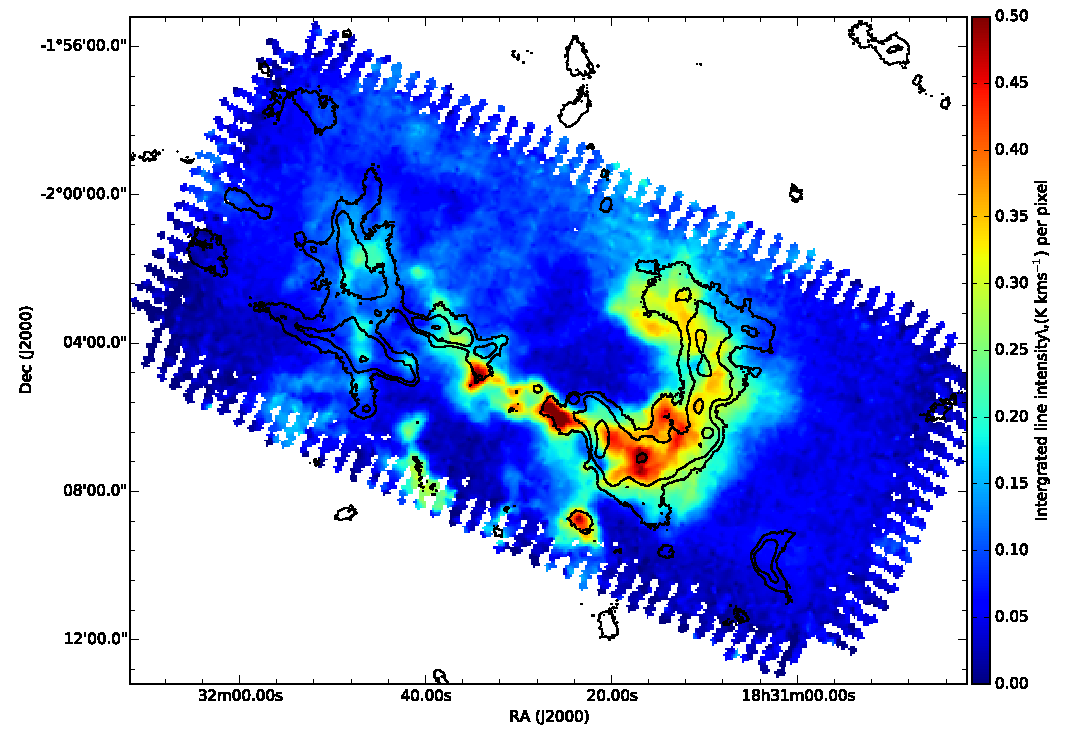
\includegraphics[scale=1]{c3/figs/20150805_W40_CO.pdf}
\caption{$^{12}$CO 3\hbox{--}2 integrated intensity map over the entire range (colour scale over -90 to +100\,km s$^{-1}$) of the central region of the W40 complex. Contours show SCUBA-2 850\,$\micron$ emission at the 5$\sigma$, 15$\sigma$ and 50$\sigma$ levels.} 
\label{fig:CO}
\end{centering}
\end{figure*} 


\subsubsection{Contamination results}

Integrated intensity maps of $^{12}\textrm{CO}$ 3\hbox{--}2 emission are subtracted from 
the original SCUBA-2 850\,$\micron$ maps using a joint data reduction process before a 
4\arcmin\ filter is applied following the method outlined in Appendix B. The fraction of 
SCUBA-2 emission that can be accounted for by $^{12}\textrm{CO}$ 3\hbox{--}2 line 
emission is presented in Figure \ref{fig:COconamination}. Contamination in W40-N is 
minimal with levels up to 5\%. The Dust Arc has significantly more contamination at the 
level of 10\%, reaching up to 20\% at its highest. 

Figure \ref{fig:COfilter} shows the distribution of flux ratios (Equation \ref{eqn:temp} and the method 
given in Appendix A) with and without CO contamination contributing to 850\,$\micron$, showing how 
even a small degree of CO contamination can have a significant effect on measuring the temperature 
of the cloud, increasing the modal flux ratio from 6.8 to 7.8 when CO is subtracted. Furthermore, the 
FWHM of the distribution increases from 1.9 to 2.8. Subtracting CO from our maps increases the 
mean and standard deviation of temperature in regions where $^{12}\textrm{CO}$ 3\hbox{--}2 is 
detected, in comparison with temperatures derived from uncorrected maps. The distribution of flux 
ratios across the map, with and without the CO contamination, are compared and found to have a 
KS-statistic of 0.253, corresponding to 1.3\% probability that the two samples are drawn from the 
same parent sample. CO contamination in the W40 complex is having a significant impact on 
distribution of flux ratios. 

\begin{figure}
\begin{centering}
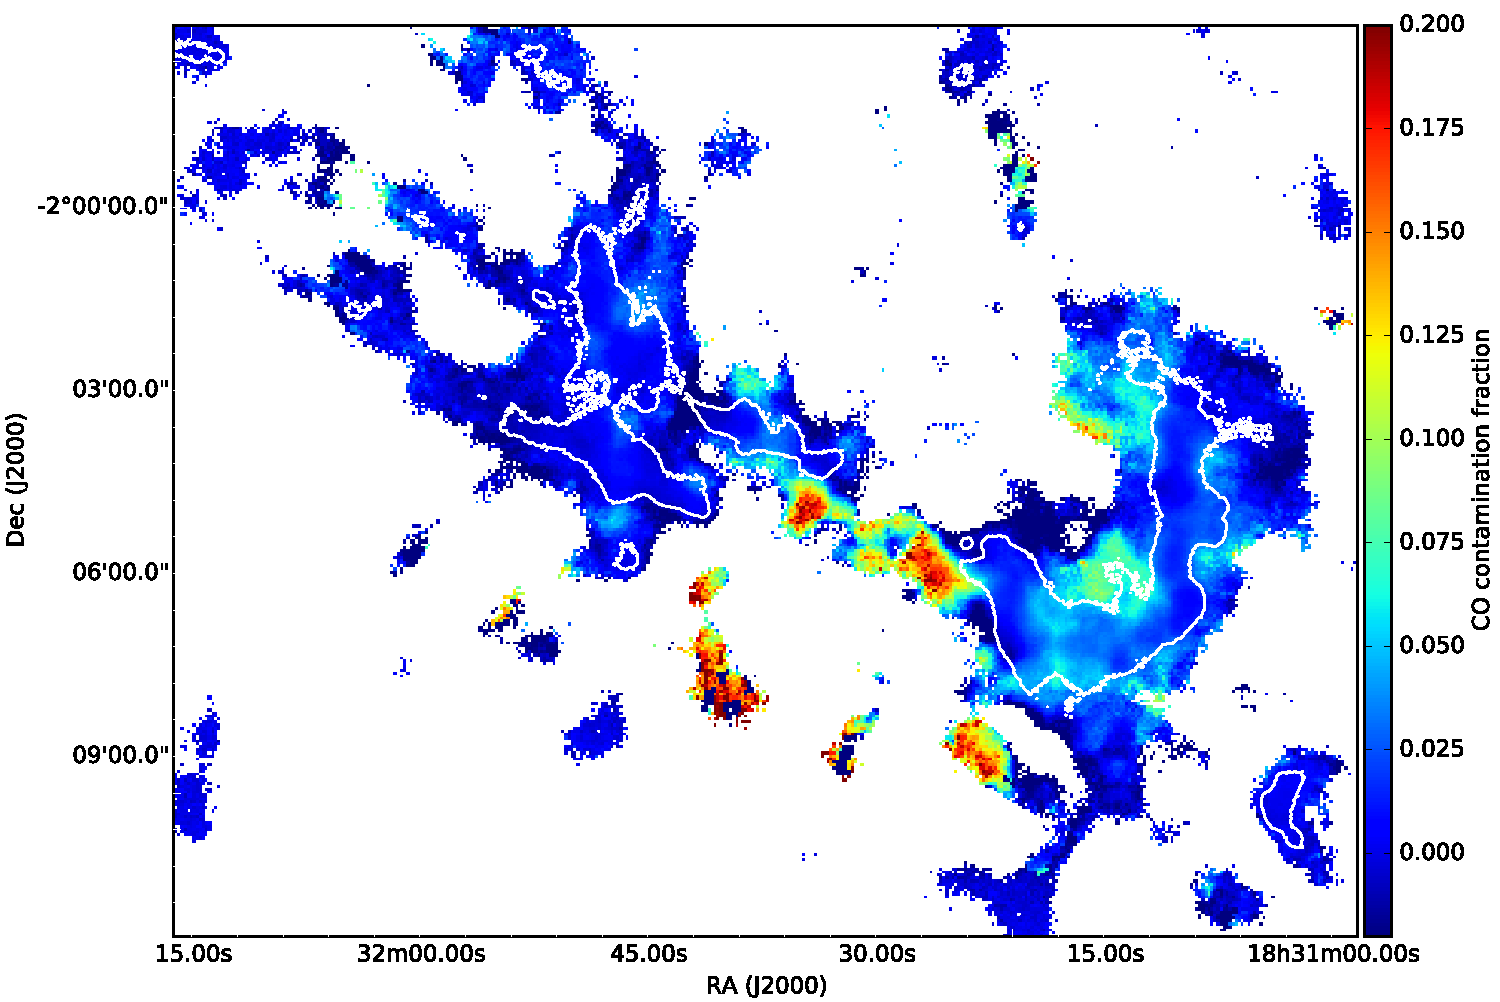
\includegraphics[scale=0.35]{c3/figs/20150804_COcontamination.pdf}
\caption{The fraction of SCUBA-2 850\,$\micron$ that can be attributed to $^{12}\textrm{CO}$ 3\hbox{--}2 345\,GHz line emission. The SCUBA-2 data are masked at 3$\sigma$ and the 5$\sigma$ level is shown in white.} 
\label{fig:COconamination}
\end{centering}
\end{figure} 

\begin{figure}
\begin{centering}
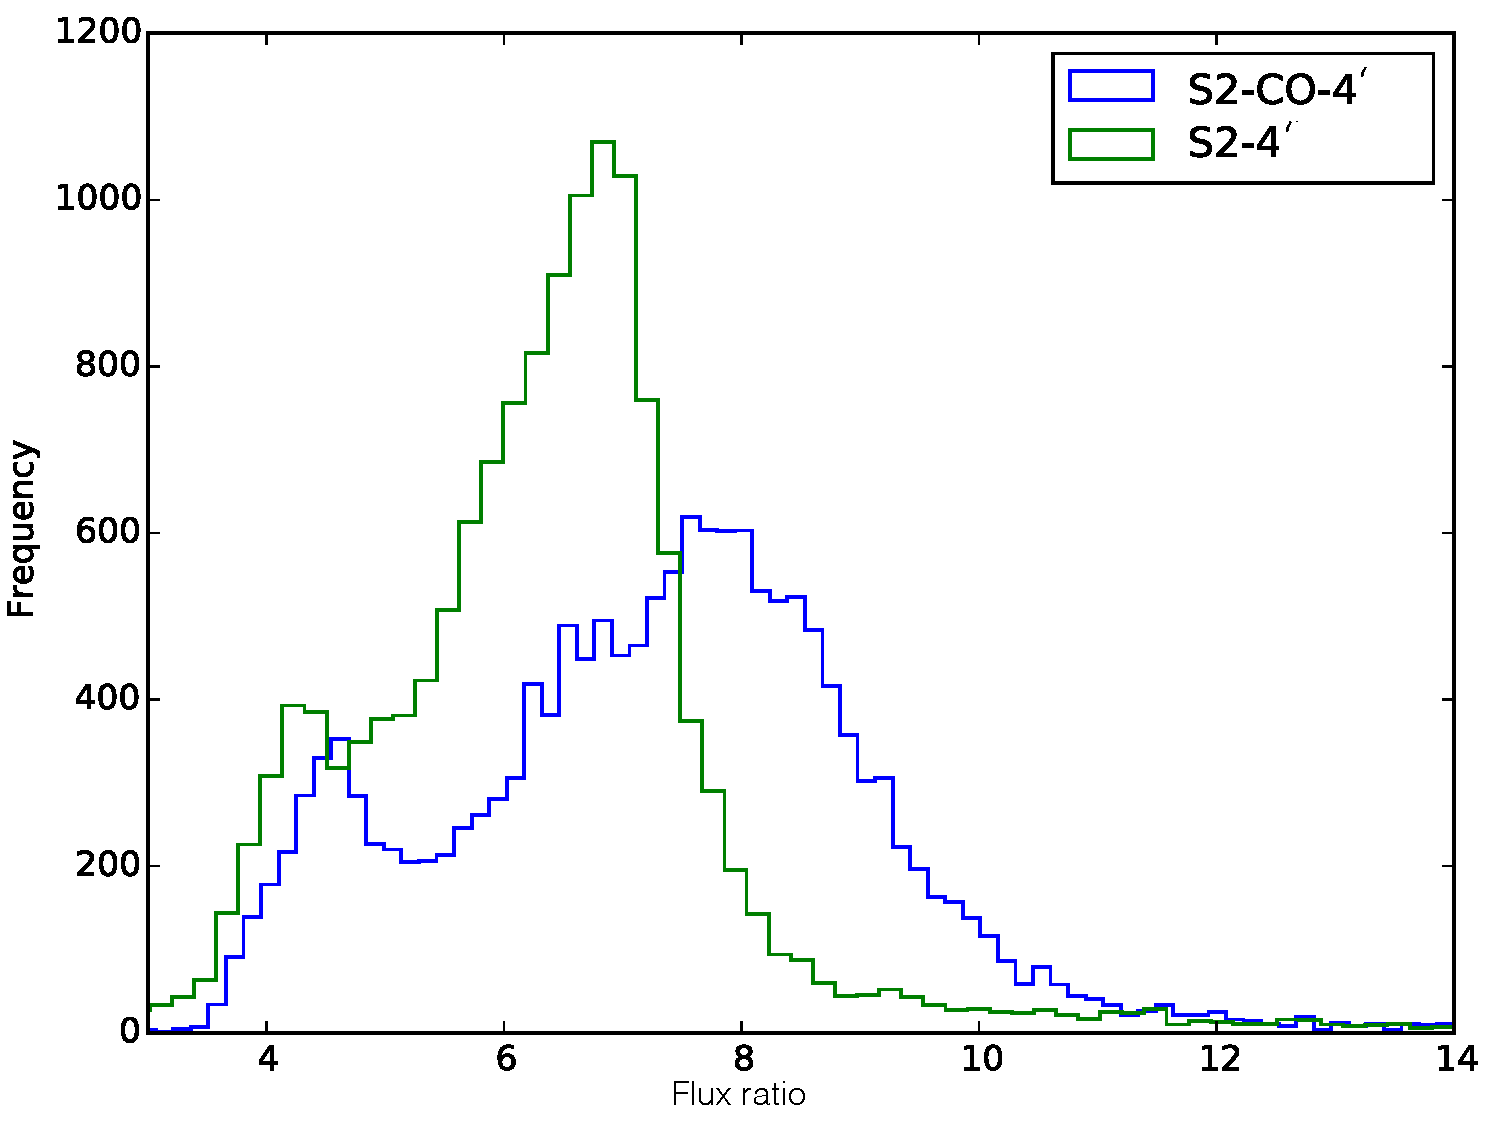
\includegraphics[scale=0.35]{c3/figs/20150804_KStest-conoco.pdf}
\caption{The distribution of 450\,$\micron$/850\,$\micron$ flux ratio for the original (blue - S2-4\arcmin) and CO subtracted (green - S2-CO-4\arcmin) Aquila reductions with additional 4\arcmin\ spatial filtering. KS-statistics reveal a 1.3\% chance that the two data sets are drawn from the same distribution.} 
\label{fig:COfilter}
\end{centering}
\end{figure} 


\subsection{Cloud velocities}

\begin{figure}
\begin{centering}
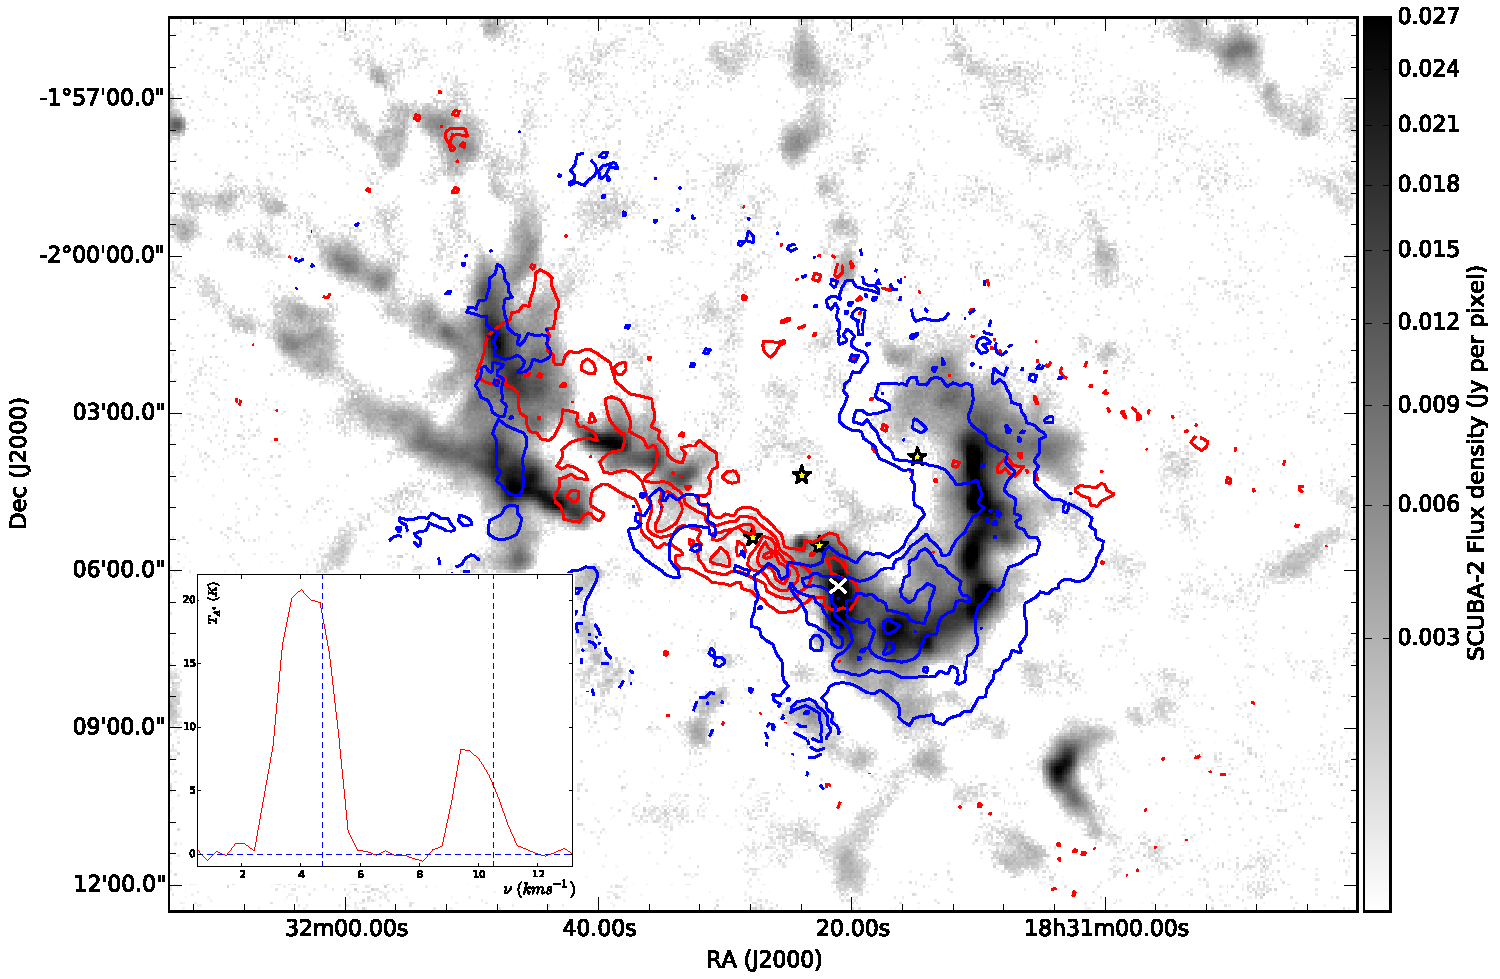
\includegraphics[scale=0.55]{c3/figs/20150904_twoclouds.pdf}
\caption{SCUBA-2 850\,$\micron$ map of the W40 complex with $^{13}\textrm{CO~2\hbox{--}1}$ integrated intensity contours of red (10km\,s$^{-1}$) and blueshifted (5km\,s$^{-1}$) emission that trace out the location of two separate clouds within the region. Blue contours are at 20, 40, 60, 80 K km\,s$^{-1}$ and red are the same levels with an additional contour at 5K km\,s$^{-1}$. The greyscale SCUBA-2 850\,$\micron$ shown here has not had CO emission subtracted. Yellow stars mark the location of the OB stars in the W40 complex. The insert shows the line emission spectra at the position of peak SCUBA-2 luminosity, marked with a white cross. Two CO clouds are visible at 5 and 10 km\,s$^{-1}$ with a significant vacancy at 7 km\,s$^{-1}$ where Shimoikura et al. 2015 finds $\textrm{HCO~4\hbox{--}3}$ emission, indicating that our $^{13}\textrm{CO~2\hbox{--}1}$ absence is due to optical depth and self-absorption.} 
\label{fig:2clouds}
\end{centering}
\end{figure} 


Two distinct components are visible in the velocity space of the $^{13}\textrm{CO~2\hbox{--}1}$ cube and are presented in Figure D1. A blueshifted component is observed at approximately 5km\,s$^{-1}$ (consistent with Zeilik & Lada 1978 and Shimoikura et al. 2015) with peak integrated flux of 88K km\,s$^{-1}$ that is coincident with the SCUBA-2 emission in the Dust Arc and, to a lesser extent, W40-N. A redshifted component is observed at approximately 10 km\,s$^{-1}$ with an integrated flux of 86 K km\,s$^{-1}$ and tightly traces a low luminosity filament of SCUBA-2 emission between W40-N and the Dust Arc, passing through the location of the OB association in the W40 complex.

Atacama Submillimeter Telescope Experiment (ASTE) observations by \cite{Shimoikura:2015kx} provides evidence of a third velocity of approximately 7 km\,s$^{-1}$ observed in $\textrm{HCO~4\hbox{--}3}$ at the submilimetre peak of the cloud (their Figure 2). $\textrm{HCO~4\hbox{--}3}$ remains optically thin at high column densities where $^{13}\textrm{CO~2\hbox{--}1}$ may become optically thick. \cite{Shimoikura:2015kx} argue that the sharp partition between 5 and 10km\,s$^{-1}$, as seen in the insert of Figure D1, may be due a dense cloud at 7 km\,s$^{-1}$ in which $^{13}\textrm{CO~2\hbox{--}1}$ is extincted but $\textrm{HCO~4\hbox{--}3}$ is observed.

Our observations of 5 and 10 km\,s$^{-1}$ $^{13}\textrm{CO~2\hbox{--}1}$ componentsare consistent with \cite{Shimoikura:2015kx}'s interpretation of a molecular shell, swept up and heated by the expanding \HII\ region, with divergent velocities either side of the shell. We find less evidence to support their claim that the ambient gas in the W40 complex has a velocity of 7 km\,s$^{-1}$ as we detect no $^{13}\textrm{CO~2\hbox{--}1}$ at that velocity in the relatively low density filaments that are significantly outside of the \HII\ shell. It is unlikely that this component extends to our off position (RA (J2000) = 18:33:29.0, Dec. (J2000) = -02:03:45.4) as it was throughly examined in \cite{Zeilik:1978qf}'s $^{12}\textrm{CO~1\hbox{--}0}$ observations and found to be clear.

HARP data are found to contain two clouds at 5 km\,s$^{-1}$ and 10km\,s$^{-1}$ that trace different morphological structures (Figure D1). The redshifted filament starts in W40-N and traces a line from this cloud to the tip of the Dust Arc. The emission from $^{13}\textrm{CO~2\hbox{--}1}$ is observed in SCUBA-2 850\,$\micron$ data and closely fits the HARP data, albeit at high SNRs, as shown in Figures D1 and 19. The red filament passes directly through the stellar cluster, enveloping the location of OS1a and the \HII\ region, as shown in Figure 19.

Since CO is photo-dissociated in \HII\ regions, the red filament is either shielding CO gas from the UV photons, or it is located in the foreground or background of the \HII\ region. SCUBA-2 does not detect a significant dust filament coincident with redshifted the CO and therefore we discount the former premise. Furthermore, figure 19 shows how clumps W40-SMM 12, 13, 20, 21, 23 and 39 are coincident both with the bright rimmed clouds (BRCs) observed in Herschel 70\,$\micron$ data and peaks of redshifted CO emission, confirming that the CO gas is within the nebulosity. This picture is consistent with the findings of \cite{Shimoikura:2015kx} who suggested the redshifted filament is a shell of heated CO gas swept up in the expanding shockwave around the \HII\ region.

\subsection{Outflow analysis}

\begin{figure*}
\begin{centering}
\begin{tabular}{l}
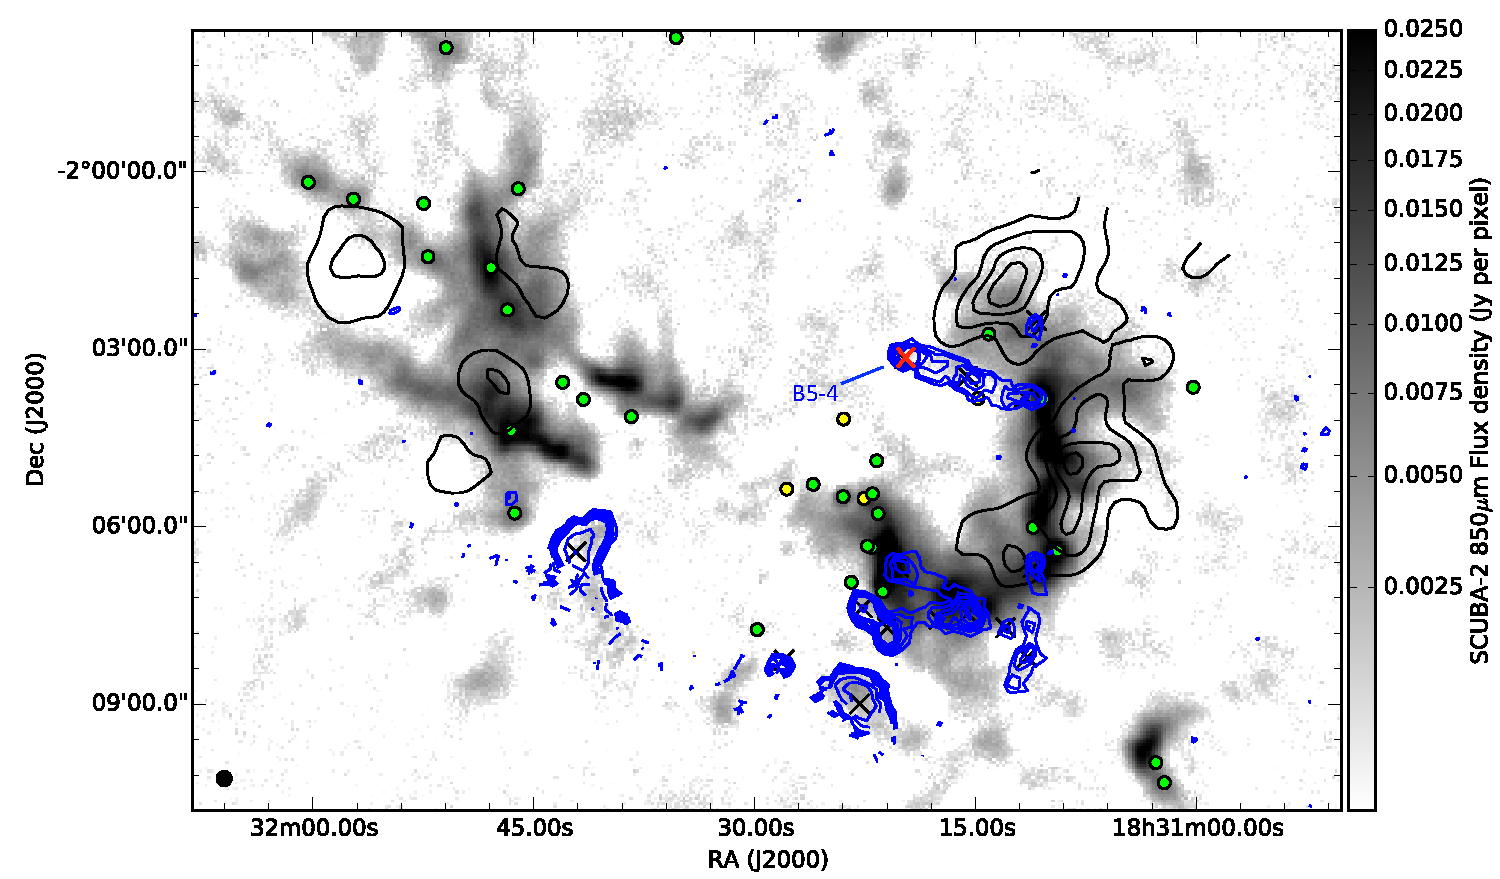
\includegraphics[scale=0.55]{c3/figs/20150903_5kmsoutflow_map.pdf} &
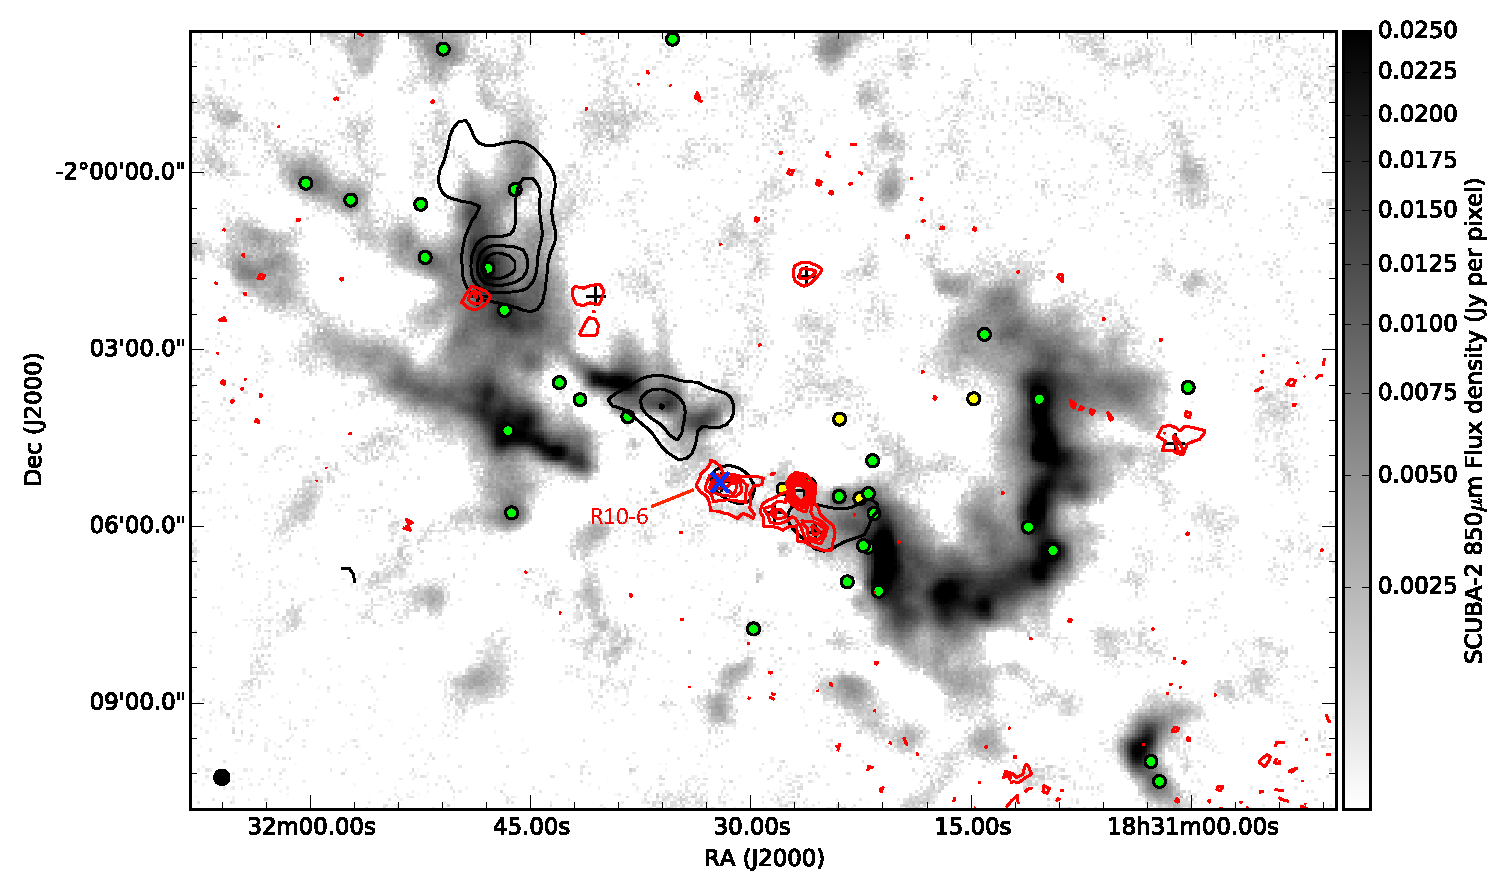
\includegraphics[scale=0.55]{c3/figs/20150903_10kmsoutflow_map.pdf} &
\end{tabular}
\caption{2CO 3�2 integrated line emission in the blue wing of the 5 km\,s$^{-1}$ (upper), and red wing of the 10\,km\,s$^{-1}$ cloud (lower). The blue 5\,km\,s$^{-1}$ wing is integrated over the velocity range 3.2$\leq$v$_{LSR}$$\leq$2.8km\,s$^{-1}$. The red 10\.km\,s$^{-1}$ wing is integrated over the velocity range 11.7$\leq$v$_{LSR}$$\leq$14.5\,km\,s$^{-1}$. Line wing sources are identified from local peaks in emission, identified as black crosses in the respective plots. Yellow stars and green circles indicate the location of the OB stars and protostars (from our composite YSOc catalogue). The grayscale backdrop map is SCUBA-2 850\,$\micron$ flux density. The black, smoothed contour represents emission from the alternative line wing (see text for velocity ranges).}
\label{fig:linewings}
\end{centering}
\end{figure*} 

\begin{figure*}
\begin{centering}
\begin{tabular}{l}
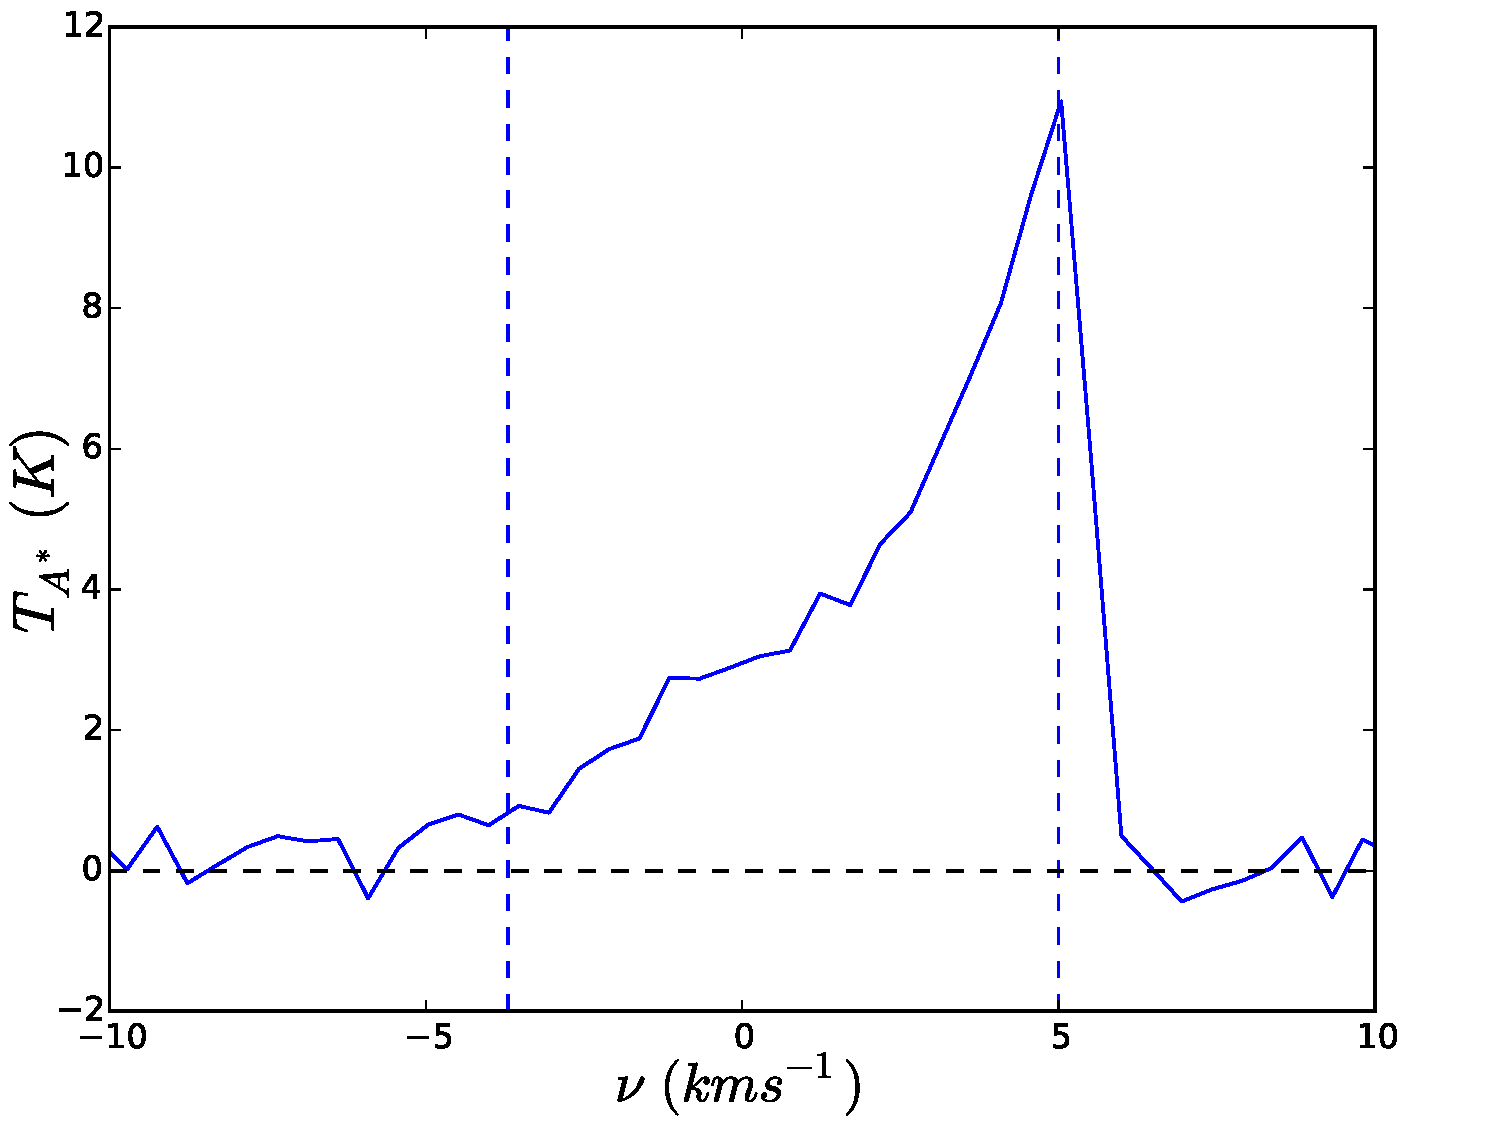
\includegraphics[scale=0.3]{c3/figs/B5-4outflow.pdf}
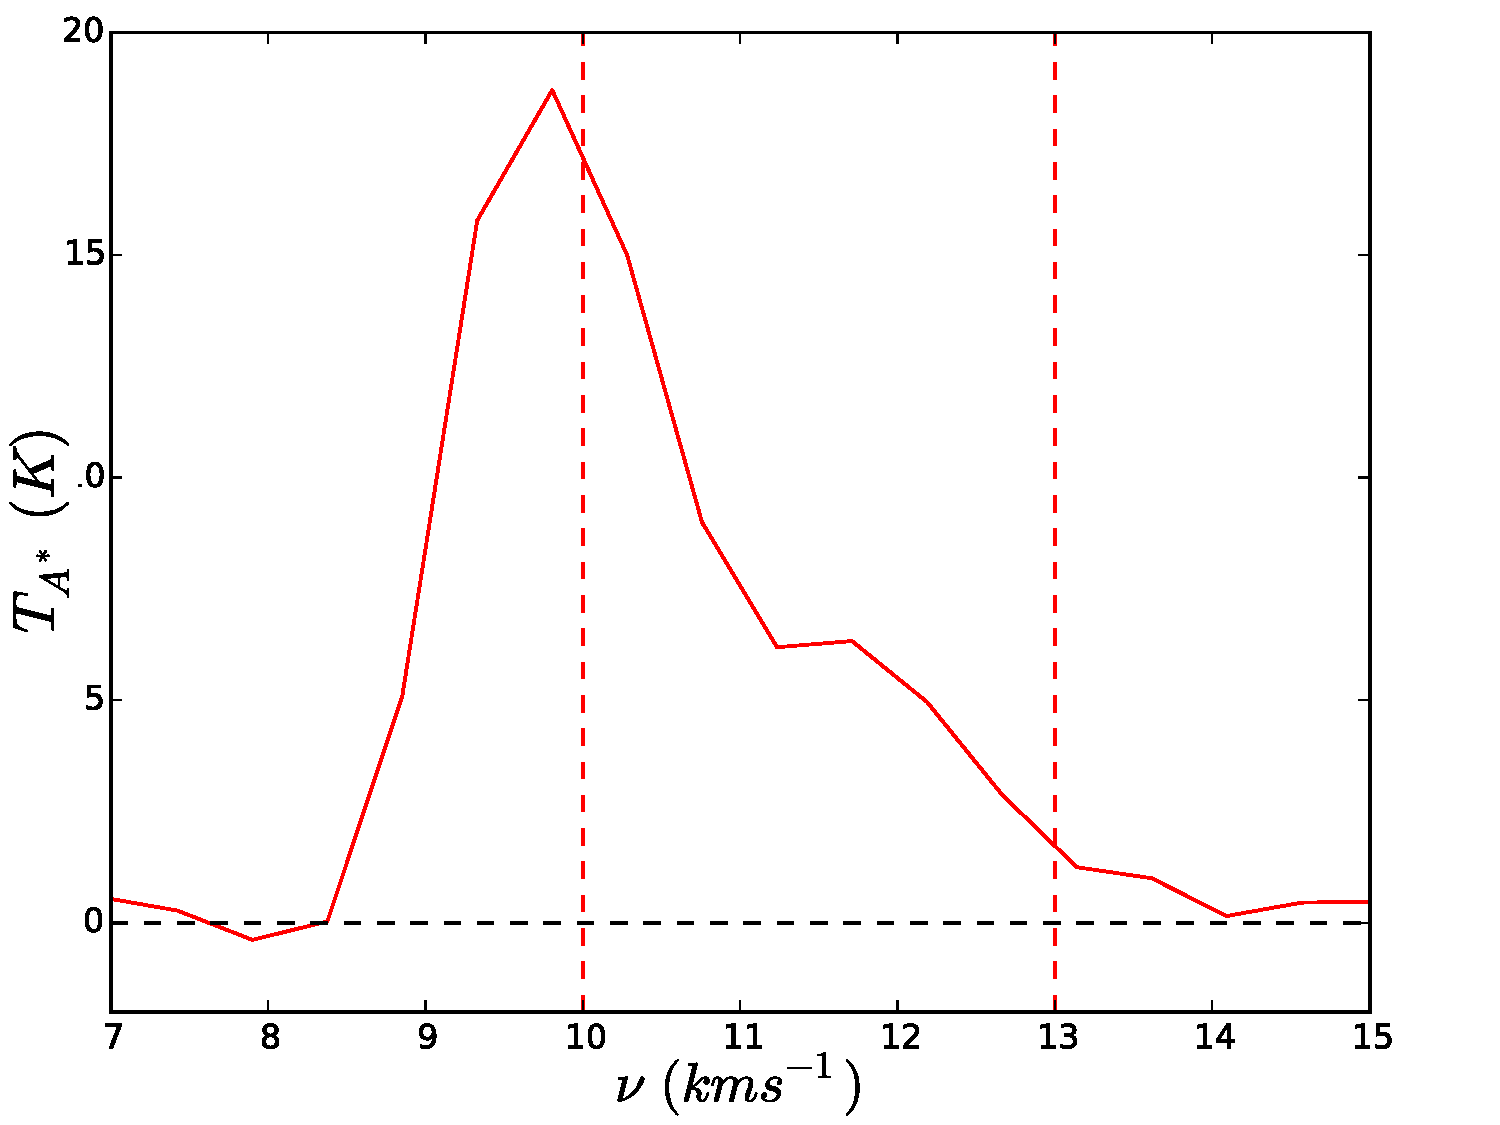
\includegraphics[scale=0.3]{c3/figs/R10-6outflow.pdf}
\end{tabular}
\caption{$^{13}\textrm{CO~2\hbox{--}1}$ line profiles of example outflows R10-6 (left) and B5-4 (right) with their locations in the 10 and 5 km\,s$^{-1}$ clouds respectively marked in Figure E1. Each profile shows prominent outflow line-wings that are either red or blue shifted. Dotted lines demonstrate the length of the line-wing, from local cloud velocity to its maximum extent.}
\label{fig:outflowslines}
\end{centering}
\end{figure*} 

A first wave of $^{12}\textrm{CO~1\hbox{--}0}$ observations of the W40 complex was made by \cite{Zeilik:1978qf} who found an ambient cloud with extended emission symptomatic of outflows with a local standard of rest velocity across the region of approximately 4.5km\,s$^{-1}$. Evidence of a weak molecular outflow was found by \cite{Zhu:2006ee}.

The complex nature of redand blue-shifted emission in the W40 complex makes direct analysis of individual outflows very difficult. We instead refer to the method of identifying local peaks in $^{13}\textrm{CO~2\hbox{--}1}$ integrated over the velocity ranges redand blue-ward of the 5 km\,s$^{-1}$ and 10 km\,s$^{-1}$ components, respectively, as used by \cite{Shimoikura:2015kx}. Peaks can be used to identify molecular outflows from protostars where the line profile shows a line-wing similar to those observed by \cite{Graves:2010mb} in Serpens Main. This method is also sensitive to the bulk motion of shocked gas around the shell of the \HII\ region, local variations in ambient gas velocity and foreground clouds at different velocity. Multiple outflow features in the �outer' velocity ranges (-3.2$\leq$v$_{LSR}$$\leq$2.8 km\,s$^{-1}$ and 11.7$\leq$v$_{LSR}$$\leq$14.5 km\,s$^{-1}$) are detected (Figure E1). The `inner' regions (5.7$\leq$v$_{LSR}$$\leq$8.4 km\,s$^{-1}$ and 8.5$\leq$v$_{LSR}$ $\leq$9.2 km\,s$^{-1}$) are where paired outflows would be expected, however \cite{Shimoikura:2015kx} outlines how $^{13}\textrm{CO~2\hbox{--}1}$ emission becomes optically thick due to a dense cloud at 7km\,s$^{-1}$, and subsequently heavily extincts any outflows in this region of the spectrum.

We detect 15 blue objects in the 5 km\,s$^{-1}$ component and nine red objects in the 10 km\,s$^{-1}$ component. These detections are almost twice the number detected by \cite{Shimoikura:2015kx}, primarily as a result of the higher resolution of the JCMT. Of this total, five are confirmed as outflows using the criterion of \cite{Hatchell:2007ly}, whereby the line wing is required to have an intensity greater than 3$\sigma$ at $\pm$3km\,s$^{-1}$ from the bulk cloud. The two most significant outflows of each cloud are presented in Figure E2. R10-6 and B5-4 have linewing widths of 3.5 km\,s$^{-1}$ 8.7 km\,s$^{-1}$, respectively. A further seven candidate outflows have a notable asymmetry in their line profiles but have too much noise to be confirmed. Eight objects are displaced components with no line asymmetries or wing-like features. Three are noise artefacts or have very low SNRs.

Of the 12 outflow-like detections, 11 have nearby protostars identified in our composite YSO catalogue (Figure E1). Due to the complexity of the region and lack of observations from the �inner' wings of the cloud it would be premature to infer that the completeness of our Class 0/I protostellar population is near 100\%. We conclude that the 10 km\,s$^{-1}$ CO filament is likely shocked shell material around the \HII\ region and we cannot rule this shell out as a source of many of the weaker candidate outflows near OS1a and IRS 5.
There is evidence that significantly powerful protostellar outflows can contribute additional localised heating of dust through shocks \citep{Buckle:2015vn}. Outflows have been detected in the W40 complex by \cite{Zeilik:1978qf} and more recently \cite{van-der-Wiel:2014vn} found red and blue shifted line wings in the eastern Dust Arc. Our HARP data extend this coverage to the whole of the Dust Arc and W40-N (Figure 3).

We detect 12 potential molecular outflows which are presented in Figure E1. The highest velocity line-wing offset is 8.7km\,s$^{-1}$ and is recorded in outflow B5-4 which is associated with a protostar in W40-SMM2. Line-wings found in Serpens Main by \cite{Graves:2010mb} are detected out to -30 km\,s$^{-1}$ and +37 km\,s$^{-1}$ from an ambient cloud of similar velocities to the W40 complex. We conclude that the outflows in the W40 complex are relatively weak and that the radiative heating from outflows is negligible, relative to the levels of the radiative feedback from the protostar itself.

We conclude that many of the line-wing detections in Figure E1 are likely caused by shocks related to this wave as opposed to protostellar outflows.

Some of the most prominent outflows we detect are found in the western Dust Arc. For example, Figure E1 shows the outflow B5-4 subtending 3\arcsec\ (0.43 pc) in length from the the protostar W40-MM5 \citep{Maury:2011ys} in W40-SMM3. As discussed in Section 6.1[UPDATE], the size of these linewings are not particularly exceptional. Given a clump mass of 12.5$\pm$2.6\,M$_{\odot}$ , we would anticipate low-to-intermediate mass star-formation is occurring. W40-SMM2 is the only significant clump in the western Dust Arc that does not have a protostar recorded in our composite YSO catalogue. In addition, no significant CO line-wing emission is detected, suggesting that this clump is indeed starless.

The $^{13}\textrm{CO~2\hbox{--}1}$ emission (Figure E1) shows many line-wing sources to the north and south of W40-SMM1 from both the 5 and 10 km\,s$^{-1}$ clouds. It is not possible to assign individual outflows to protostars, or to rule out that the line-wings could be caused by shocked gas swept up in a shell where the \HII\ region interacts with the filament. The absence of CO line-wing sources in the vicinity of the YSOs near OS2b does suggest that either; these are particularly low-mass protostars with weak outflows, the majority of the $^{13}\textrm{CO~2\hbox{--}1}$ has been photo-ionised by the \HII\ region, or that the protostars detected here are false detections.

\section{Conclusions}


\begin{enumerate}
\item We find evidence for significant levels of $^{12}$CO 3\hbox{--}2 line emission in 
HARP data that contaminates the 850\,$\micron$ band range between 3 and 10\% in 
the majority of the filaments. In a minority of areas contamination reaches up to 20\%. 
Removing the $^{12}$CO 3\hbox{--}2 contamination significantly increases the 
calculated dust temperatures, beyond the calculated uncertainties. 
\end{enumerate}
 
   % Free-Free contamination
   \chapter{Free-Free contamination}
\label{ch:chapter4}

%W40 - intro preamble 
In this chapter we examine the arguments for a thermal Bremsstrahlung, or free-free, 
contribution to the SCUBA-2 detections, addressing questions regarding the source, 
strength, spectral index, and location of the turnover (from partially opaque to optically 
thin) of free-free emission. We examine the various sources of free-free emission in 
the JCMT GBS and asses the magnitude of the contribution of free-free to SCUBA-2 
bands.

\section{Introduction to thermal breemstralung emission}

%NEW - background theory
Thermal Bremsstrahlung, or free-free, emission is a thermal process by which photons are produced from electron scatter in a plasma in LTE. We derive the spectral index of the free-free emission by first considering the number of electrons, $N_{e}$, passing an ion, per unit time. The electrons have a speed range $v$ to $v + dv$ and the the ion has an impact parameter of $b$ to $b + db$ such that 
\begin{equation}
N_{e}(2\pi b\,db)vf(v)\,dv. \label{eqn:ion}
\end{equation}
In this system the number of `encounters', $N(v,b)$, between the ion and an electron, per unit volume, per unit time, is 
\begin{equation}
N(v,b)\,dv\,db = (2\pi\,db)[vf(v)]N_{e}N_{i}, \label{eqn:encounters}
\end{equation}
and the average energy per unit frequency, $W_{\nu}$, is 
\begin{equation}
W_{\nu}\approx \frac{\pi^{2}}{2}\frac{Z^{2}e^{6}}{c^{3}m_{e}^2}\left ( \frac{1}{b^{2}v^{2}} \right ) 
\label{eqn:energy}
\end{equation}
where the above constants have their usual meanings. From radiative transfer, the emission coefficient, $\epsilon _{\nu}$, can be calculated by integrating energy and encounters over $b$ and $v$ as such, 
\begin{equation}
4\pi\epsilon _{\nu}=\int_{b=0}^{\infty }\int_{v=0}^{\infty }W_{v}(v,b)N(v,b)\,dv\,db. \label{eqn:epsilon} 
\end{equation}
Considering non-relativistic Maxwellian distribution of electron velocities,  
\begin{equation}
f(v)=\frac{4v^{2}}{\sqrt{\pi }}\left ( \frac{m_{e}}{2k_{B}T_{e}} \right )^{3/2}exp\left (- \frac{m_{e}v^{2}}{2k_{B}T_{e}} \right ), \label{eqn:max}
\end{equation}
the free-free emission coefficient can be derived as 
\begin{equation}
\epsilon _{\nu}=\frac{\pi^{2}Z^{2}e^{6}N_{e}N_{i}}{4c^{3}m_{e}^{2}}\left ( \frac{2m_{e}}{\pi\,k_{B}T_{e}} \right )^{1/2}ln\left ( \frac{b_{max}}{b_{min}} \right ).
\label{eqn:eff}
\end{equation}
The minimum and maximum impact parameters, $b_{min}(v)$ and $b_{max}(v,\nu)$, make up the Gaunt factor, 
\begin{equation}
g_{ff}(\nu,T) = \frac{\sqrt{3}}{\pi}ln\left (\frac{b_{max}}{b_{min}} \right), 
\label{eqn:gaunt}
\end{equation}
that value of which ranges as $g_{ff}(\nu)\propto 1/\nu$ between 1 and 10 across the radio spectrum. Using Kirchoff's law ($\kappa_\nu=\epsilon_{\nu} / B_{\nu}(T)$) the absorption coefficient, $\kappa_\nu$, can be calculated in the Rayleigh-Jeans limit as 
\begin{equation}
\kappa_\nu=\frac{1}{\nu^{2}T^{3/2}}\frac{\pi^{3}}{\sqrt{48}}\,g_{ff}\left [ \frac{Z^{2}e^{6}}{c}N_{e}N_{i}\frac{1}{\sqrt{2\pi\,(m_{e}k_{B})^{3}}} \right ].
\label{eqn:kappaff}
\end{equation}
Because the Gaunt factor is weakly inversely proportional to frequency the opacity of free-free emission can be approximated to $\kappa_\nu \propto \nu^{-2.1}$ \citep{Oster:1961fk, Altenhoff:1970ai} and as a result the optical depth of the free-free can be written as 
\begin{equation}
\tau_\nu \approx \int \frac{N_{e}^{2}}{\nu^{2.1}T^{3/2}}\,ds.
\label{eqn:Tauff}
\end{equation}
From this expression it can be determined that at low frequencies $\tau_\nu \gg 1$ and emission will become optically thick. Likewise at very high frequencies emission will become optically, $\tau_\nu \ll 1$. Considering the equation of flux density from radiative transfer, 
\begin{equation}
S_\nu= \int_{\Omega }B_{\nu}(T,\nu)\tau\,d\Omega, 
\label{eqn:Snu}
\end{equation}
it is possible to show that free-free emission at very low frequencies will resemble a black body where $S_\nu \propto \nu^{2}$. Likewise at very high frequencies free-free emission is approximately flat, $S_\nu \propto \nu^{-0.1}$ \citep{Mezger:1967fk}.

%NEW-turnover
At $\tau_\nu = 1$ free-free emission will undergo a `turnover' from the optically thick to thin regime, typically at low frequencies around KHz regime.  At very high frequencies another break occurs in the spectrum when $h\nu \gg k_{B}T_{e}$ and the free-free spectrum goes from flat to an exponential decay that is described by, 
\begin{equation}
J_{\nu,T} \propto T^{-1/2}exp\left ( \frac{-h\nu}{k_{B}T_{e}}\right) N_{e}^{2} g_{ff}(\nu,T), 
\label{eqn:expdecay}
\end{equation}
where $J_{\nu,T}$ is the emissivity [CITE]. For a electron temperature of $10^{4}$\,K, the exponential decay break can be estimated at occurring short ward of 1\,$\micron$. 

\section{\HII\ observations}
%W40
\begin{figure}
\begin{centering}
\includegraphics[scale=0.5]{/Users/damian/Documents/Thesis_et_al/Papers/starformation_in_W40/W40images/20150904_W40Hiiregion.pdf}
\caption{Archival VLA 21\,cm NRAO VLA Sky Survey \citep{Condon:1998kx} continuum map of the W40 complex \HII region (45\arcsec\ resolution). Red  \emph{Herschel} 70$\micron$ contours of the nebulosity SH-64 at 300, 1200, 4800, 12000\,MJy/Sr. Blue SCUBA-2 850\,$\micron$ 
contours of the dust cloud at the 5$\sigma$ level. Yellow stars indicate the locations of the OB stars, with the O9.5 star OS1 the primary ionising object of the region. The white cross indicates the peak of the VLA 21\,cm emission.} 
\label{fig:21cm}
\end{centering}
\end{figure} 

%NEW - lyman photons
In star formation, free-free emission is typically observed from H\,\textsc{ii} regions formed by photoionisation of molecular hydrogen by UV photons from B4V stars or earlier. The UV, or Lyman, photon density, $N_{Ly}$,  required to maintain the ionisation of an \HII\ region is given by \cite{Kurtz:1994cr} as 
\begin{equation}
N_{Ly} \geq 8.04\times10^{46}T_{e}^{-0.85}U^{3}, 
\label{eqn:lyman}
\end{equation}
where U is the excitation parameter $R_{s}N_{e}^{2/3}$ for a Stromgern sphere of radius $R_{s}$. These two variables are also related through 
\begin{equation}
N_{Ly} = \alpha _HN_e^{2}\frac{4}{3}\pi\,R_s^3
\label{eqn:stromgern}
\end{equation}
where $\alpha _H$ is the hydrogen recombination rate, approximately equal to 3$\times$10$^{-13}$\,cm$^{3}$\,s$^{-1}$. \HII\ regions are large scale, low density structures with radii greater than $10^{18}$\,cm and $N_{e}$ less than $10^{4}$\,cm$^{-3}$. The stellar $N^{*}_{Ly}$ for the OB stars capable of producing \HII\ regions is typically greater than $10^{46}$\,cm$^{-3}$. By considering $N^{*}_{Ly}$ at specific frequencies \cite{Kurtz:1994cr} calculates the flux density that would be observed if viewing an \HII\ region at a distance, $d$, using 
\begin{equation}
S_{\nu}(\mathrm{Jy}) = 1.32\times10^{-49}\xi N^{*}_{Ly}a(\nu,T)\left ( \frac{\nu}{\mathrm{GHz}} \right )^{-0.1}\left ( \frac{T_{e}}{\mathrm{K}} \right )^{0.5}\left ( \frac{d}{\mathrm{kpc}} \right )^{-2},
\label{eqn:kurtz}
\end{equation}
where a$(\nu,T)$ is a constant equal to 0.98 \citep{Mezger:1967fk} and $\xi$ is the fraction of UV photons not absorbed by the dust set at 10\%. Free-free emission from large scale, diffuse H\,\textsc{ii} regions is predicated to be optically thin at radio frequencies emission where the power law becomes approximately flat with an $\alpha_{\mathrm{ff}}$ = -0.1 \citep{Oster:1961fk, Mezger:1967fk}. 

%\NEW - general info on Hii regions
In an \HII\ region UV heat up the gasses and plasma of the ISM by radiative transfer to temperatures in excess of 10000\,K. This causes the exposed material to expand adiabatically into the space surround the OB star/s. In the transition zone between the \HII\ region and the neutral ISM two fronts are observed; the ionisation front [CITE] and the shock [CITE]. In the shock front, expansion of the \HII\ region is thought to sweep up the ISM producing localised over densities associated with a `shell' of material around the \HII\ region [CITE]. Whether the shock front has sufficient pressure to destabilise existing cores within any exposed filaments and `trigger' star-formation is an open question \citep{Lefloch:1994uq, Urquhart:2009dq}. The ionisation front represents a region where neutral material is being ionised through exposure to UV photons. Rate of ionisation is heavily dependant on the local density. High density regions take considerably longer to break down than lower density regions and as a result `champagne' flows \citep{Dale:2012fk} are observed where the molecular cloud has been ruptured by an internal \HII\ and photons are exiting through a narrow opening. The \HII\ region can be further imbedded by accretion flow of neutral material onto the star \cite{Dale:2005kx, Dale:2011vn} and by gravity when at the centre of massive cloud \cite{Yorke:1989ys}. The region in-between the ionisation front and shock front is collectively known as a photo-dissociative region (PDR, \citeauthor{Thompson:2004uq} \citeyear{Thompson:2004uq}). An example of a PDR is observed in Perseus, a star forming region observed as part of the JCMT GBS.   

\section{\UCHII\ observations}

 %W40
\begin{figure*}
\begin{centering}
\begin{tabular}{l}
\includegraphics[scale=0.28]{/Users/damian/Documents/Thesis_et_al/Papers/starformation_in_W40/W40images/free-free-alpha-sketch.pdf}
\includegraphics[scale=0.28]{/Users/damian/Documents/Thesis_et_al/Papers/starformation_in_W40/W40images/20150506_freefreecutoff.pdf}
\end{tabular}
\caption{\textbf{Left]} A schematic of the SED shape for three hypothetical scenarios of{fig:freefreealpha} free-free emission. %\\
\textbf{Case a)} an UCH\,\textsc{ii} with $\alpha_{\mathrm{ff}}$ = 0.6 has a turnover that occurs short ward of the submillimetre regime, and as a result has a majority contribution to the 850\,$\micron$ band and a significant contribution to the 450\,$\micron$ band. %\\
\textbf{Case b)} a YSO emits free-free emission, $\alpha_{\mathrm{ff}}$ = 1.0, from a collimated jet. However the spectrum turns over to the optically thin regime long ward of submillimetre wavelengths, and consequently free-free emission contributes roughly equally to both SCUBA-2 bands. %\\
\textbf{Case c)} a H\,\textsc{ii} region has free-free emission from diffuse gas of $\alpha_{\mathrm{ff}}$ = -0.1 that outshines that from compact objects at long wavelengths. However, the flat spectrum means that at submillimetre wavelengths the emission is all but negligible.
\textbf{Right]} Free-free turnover as a function of launching electron density (as described by \citeauthor{Olnon:1975bh} \citeyear{Olnon:1975bh}  in Equation \ref{eqn:turnover}). Dashed lines indicate the submillimetre regime (1.3\,mm to 350\,$\micron$).}
\label{fig:freefreealpha}
\end{centering}
\end{figure*} 

%W40 - uchii scale intro
In addition to these large scale structures, free-free emission is also detected in the form of a power law at scale sizes comparable to individual stars \citep{Panagia:1975uq}. 

%NEW - what is an UCHII
Early type OB stars undergoing mass loss through winds produce free-free emission from ionised material leaving the star, in addition to UV photons ionising the ISM, and are considered compact ($\leq$0.5$\hbox{ pc}$), ultra compact ($\leq$ 0.1$\hbox{ pc}$) and hyper compact ($\leq$ 0.03$\hbox{ pc}$) \HII\ regions \citep{Wright:1975kx, Harvey:1979qf}. These are the processors of evolved \HII\ regions (10$\hbox{ pc}$,\citeauthor{Kurtz:2005kl} \citeyear{Kurtz:2005kl}). From here on in we refer to these classes collectively as \UCHII\ regions. Whereas \HII\ regions are diffuse, homogenous fields of emission, \UCHII\ regions have an electron density is inversely proportional to radius. Assuming spherical winds of constant velocity \cite{Panagia:1975uq} and \cite{Wright:1975kx} derive the spectral index of the free-free emission as $\alpha_{\mathrm{ff}}$ = 0.6. Large surveys of \UCHII\,candidate regions are consistent with this result \citep{Harvey:1979qf, Wood:1989bh, Kurtz:1994cr, Molinari:1998dq, Walsh:1998nx, Kurtz:2005kl}.

%W40 - EDIT - turnover equ
Where the free-free emission mechanism is a spherical ionised stellar wind,Emission can be thought of as \emph{partially thick} with lower frequencies probing greater depths of emission within the wind before becoming fully optically thin at shorter wavelengths where only the diffuse \HII\ region is being observed. The exact location of this free-free turnover, $\nu_{c}$, has been much debated in the literature. If the turnover occurs short-ward of submillimetre wavelengths then it is possible that the free-free may contribute in part to SCUBA-2 observations of dust emission. \cite{Olnon:1975bh} defines $\nu_{c}$ as a function of electron density, N$_{e}$(R) = N$_{e,0}$ where r $\leq$ R, as 
\begin{equation}
\log_{10} \nu _{c} = - 0.516 + \frac{1}{2.1}\log_{10}\left ( \frac{8}{3}RN_{e,0}^{2}T_{e}^{-1.35} \right ),  
\label{eqn:turnover}
\end{equation}
where R is the launching radius of the wind (typically 10\,AU) and $T_{e}$ is the electron temperature (typically 10$^{4}$\,K). Figure \ref{fig:turnover} highlights how a turnover point short wards of the submillimetre regime requires an electron density in excess of 10$^{8}$\,cm$^{-3}$. 

%W40 - electron density expression 
The electron density n$_{0}$ is not easily determined from observations. We therefore turn to indirect measurements to make a general statement about what systems will produce free-free emission that is opaque at submillimetre wavelengths and hence may subsequently be contributing to SCUBA-2 emission. We assume that n$_{0}$ is proportional to stellar mass and by association varies with spectral class as the more massive stars are known to produce more vigorous winds and greater mass loss. \cite{Sandell:2011dz}'s results indicate that the free-free contribution is significant for early B stars in their sample, but not for late B and A class stars. MWC 297 is the lowest mass star in their sample for which free-free contributes at SCUBA-2 wavelengths and we therefore mark it as a lower limit of stellar class. MWC 297 has a luminosity of 3 $\times$ 10$^{3}$\,L$_{\odot}$ \citep{Drew:1997qf} which corresponds to a class B1.5Ve or B4V star. Given the nature of these assumptions, we are limited to assigning an upper estimate of spectral class B4V, above which the free-free turnover can occur in the submilimetre regime. 

%MWC297 - uchii summarise
\UCHII\ are associated with stars that are sufficiently massive (greater than 8$M_{\mathrm{\odot}}$) that their Kelvin-Helmholtz contraction timescale is shorter than their free fall and accretion timescale \citep{Manoj:2007ly}. These stars reach the main sequence and start producing ionising radiation whilst still embedded within their protostellar envelope \citep{McKee:2003ys}. This would then lead to a compact region of highly ionised winds, as detected by \cite{Malbet:2007zr} and \cite{Drew:1997qf}. We follow \cite{Wood:1989bh}'s description of an UCH\,\textsc{ii} region as region with electron density greater than 10$^{4}$\,cm$^{-3}$ within a diameter of less than 0.1\,pc. The minute size of the \UCHII\ region means they cannot be detected optically and are interest observed through free-free processes or the indirect heating of dust. The lifetime of the ultra-compact stage of an \HII\ region is estimated at 4$\times$10$^{5}$\,years, approximately 10\% the lifetime of a typical O star. 

\begin{figure}
\begin{centering}
\includegraphics[scale=0.4]{/Users/damian/Documents/Thesis_et_al/Papers/starformation_in_W40/W40images/20150904_freefree_small.pdf}
\caption{Archival AUI/NRAO 3.6\,cm map of the W40 complex OB association (NRAO/VLA Archive Survey, (c) 2005-2007). SCUBA-2 850\,$\micron$ contours of dust emission at 5$\sigma$, 15$\sigma$ and 50$\sigma$ overlaid. Yellow markers indicate the locations of the OB stars while cyan circles indicate the location of compact radio sources identified by Rodriguez et al 2010. Cyan crosses mark the four peaks identified separately in the AUI/NRAO 3.6\,cm map.}
\label{fig:3_6cm}
\end{centering}
\end{figure} 


\subsection{Jets}

%NEW - intro jets
A minority of radio bright young OB stars are observed with $\alpha_{\mathrm{ff}} \geq$ 0.6, for example MWC 349 \citep{Olnon:1975bh}, MWC 297 \cite{Skinner:1993bh, Sandell:2011dz} and AB Aur \citep{Rodriguez:2014zr}.
%W40
\cite{Reynolds:1986cr} provides a comprehensive examination of models for stellar winds and finds that, where the outflow is highly collimated and accelerating (as this the case of bi-polar jets) the spectral index becomes increasingly opaque with $\alpha_\mathrm{ff} \simeq$ 1.0. [CAN DERIVE IF NECESSARY BUT ITS PRETTY OVERKILL].

%W40 - example jet source
MWC 349 \citep{Tafoya:2004ly,Sandell:2011dz} and MWC 297 \citep{Sandell:2011dz, Rumble:2015vn} 
are early B-class Herbig stars where empirical observations have suggested that the free-free emission 
is sufficiently bright and opaque that it dominates over the dust emission at submillimetre wavelengths 
and produces a distinct point source in the observations consistent with a compact object. If similar 
point sources are present the SCUBA-2 observations of W40 complex, and are also consistent the 
location of whole compact radio sources, that could well signify the potential for free-free contribution.


%%%%%%%%

\section{Free-free contribution to SCUBA-2}

\begin{figure}
\begin{center}
\includegraphics[scale=0.45]{/Users/damian/Documents/Thesis_et_al/images/20140821_mwc297_free_free_SED.pdf}
\caption{The Spectral Energy Distribution of MWC 297 from submillimetre to radio wavelengths. SCUBA-2 fluxes (found using aperture photometry as described in Section 5.2.) are presented alongside those collated by \protect\cite{Sandell:2011dz} who fit a power law $\alpha = 1.03\pm0.02$, consistent with free-free emission from an UCH\textrm{II} region and polar jets or outflows.}
\label{fig:freefreeSED}
\end{center}
\end{figure}

%NEW - free-free contrib intro 
Where free-free emission is significantly bright and remains optically opaque up to submillimetre wavelengths it may be detected by SCUBA-2 in the 450 and 850\,$\micron$ bands.  

%W40 - examples of turnover issue
\cite{Harvey:1979qf}, \cite{Kurtz:1994cr} and \cite{Sandell:2011dz} present multi-wavelength radio surveys of numerous HAeBe systems. A number of A class and late B class stars have faint free-free \UCHII\ detections that appear to become optically thin long-ward of the submilimetre regime or are otherwise negligible when compared to emission at from the dust in the protostellar disc or envelope. \cite{Rodriguez:2014zr} finds evidence that free-free emission in AB Aur has index $\alpha_{\mathrm{ff}}$ = 1.1 at cm wavelengths, however flux becomes optically thin by 1.3\,mm, leading to the conclusion that  $\nu_{c} \sim$ 70\,GHz. The early B systems of MWC 349, MWC 279 and LkH$\alpha$ 101 are observed to have strong free-free wind or jet emission which fits a power law right up to the submillimetre where the free-free provides a substantial, if not the majority of emission at these wavelengths. \cite{Olnon:1975bh} calculates that $\nu_{c} \sim$ 575\,GHz for MWC 349 using Equation \ref{eqn:turnover}, given that R $\sim$ 11\,AU and N$_{e,0}$ $\sim$ 9$\times$10$^{8}$\,cm$^{-3}$ \citep{Greenstein:1973uq}. \cite{Harvey:1979qf} goes further and argues that free-free emission may be opaque up to 100\,$\micron$.

We present our methods for calculating and subtracting the free-free contribution from SCUBA-2 data published in  \cite{Rumble:2015vn} and Rumble et al. (2016, in prep.). 

\subsection{Direct methods}

\begin{figure*}
\begin{center}
\includegraphics[scale=0.5]{/Users/damian/Documents/Thesis_et_al/Papers/Starformation in MWC297/mwc297_arXiv/MNRAS/20140618_mwc297_contamination.jpeg}
\caption{IR1 SCUBA-2 850\,$\micron$ data before \emph{left} and after \emph{right} removal of free-free contamination from an UCH\textrm{II} region and polar jets/winds (represented by the point source contours in the \emph{left} plot). SCUBA-2 contours are at 0.011, 0.022, 0.033 and 0.055 Jy/pixel (corresponding to 5, 10, 15 and 25 $\sigma$ detection limits). 6\,cm VLA contours (red) from Sandell (private comm.) at 0.002, 0.005, 0.02, 0.072, 0.083 Jy/beam are overlaid on the left hand panel. The location of MWC 297 is marked with a star. Beam sizes are shown at the bottom of the image (VLA CnD config. \emph{left} and JCMT \emph{right}.) }
\label{fig:contamination}
\end{center}
\end{figure*}


%MWC 297 - MWC297
\cite{Skinner:1993bh} studied free-free 3.6\,cm and 6.0\,cm radio emission from stellar winds around the B1.5ve star MWC 297 and found a power law of the form $S_{\nu} \propto \nu^{\alpha}$ where $\alpha$ is equal to 0.6238 in the optically thin regime. \cite{Sandell:2011dz} extended the study down to 3 mm and revised the spectral index to $\alpha = 1.03\pm0.02$ which is consistent with a collimated jet component to free-free emission. The free-free power law extends into the submillimetre spectrum; however, at wavelengths shorter than 2.7\,mm there is potential for a thermal dust component in the observed flux, so submillimetre flux is not included in the calculation of $\alpha$.

%MWC 297 - VLA observations
Figure~\ref{fig:contamination} displays 6\,cm radio emission from the VLA CnD configuration in conjunction with 
SCUBA-2 850\,$\micron$ data (Skinner \citeyear{Skinner:1993bh}, Sandell priv. comm). Both sets of data show 
peaks in emission which are coincident with a point source at the location of the star MWC 297 in 1\,mm and 
3\,mm data presented by \cite{Alonso-Albi:2009ve}. The peak of the SCUBA-2 850\,$\micron$ emission in 
Figure~\ref{fig:contamination} is 86\,mJy/pixel, consistent with the SCUBA 850\,$\micron$ value of 82\,mJy/pixel 
\citep{Alonso-Albi:2009ve}.

 %MWC 297 - jets obs.
The VLA data also show extended emission to the north and south of MWC 297 which is consistent with polar 
winds or jets. The intensity of emission is significantly weaker than that of the UCH\textrm{II} region. Considering 
the elongated beam shape of the VLA CnD observations (21.1\arcsec $\times$ 5.2\arcsec, PA$ = -61^{\circ}.3$) 
accounts for much the E/W elongation of the emission. In addition to this, \cite{Manoj:2007ly} describe this emission 
as coming from within 80\,AU of MWC 297. This is much smaller than the JCMT beam and therefore we model the 
dominant free-free emission from MWC 297 as a point source.

%MWC 297 - model and subtraction
By taking the revised power law least square fit to \cite{Skinner:1993bh} and \cite{Sandell:2011dz}'s results at radio and millimetre wavelengths and extrapolating to the submillimetre wavelengths of SCUBA-2, we are able to calculate the effect of free-free emission due to a point-like UCH\textrm{II} region as an integrated flux of 934$\pm$128 mJy at 450\,$\micron$ and 471$\pm$62 mJy at 850\,$\micron$. 
%NEW
Single pixels with these values were then implanted into blank SCUBA-2 450 and 850\,$\micron$ PONGs and the map convolved with the JCMT beam to produce an SCUBA-2 free-free emission map. These are subtracted off of the original SCUBA-2 maps to leave a SCUBA-2 dust map.

%NEW - large scale intro
In addition to small scale free-free structures that are modelled as point sources, we can also run a free-free subtraction for large-scale emission from the diffuse emission from the \HII\ region.

%W40 - large-scale observations
Archival VLA 21\,cm data (45\arcsec\ resolution) is presented in Figure \ref{fig:21cm} and shows the location of the 1.7\arcmin\ large scale \HII\ region associated with SH-64 \citep{Condon:1998kx}. \cite{Rodney:2008ij} presents a summary of observations at multiple radio wavelengths and conclude a flat spectral index ($\alpha$ = -0.1) as expected from homogenous, optically thin free-free emission as predicted by \cite{Oster:1961fk} and \cite{Mezger:1967fk}.  

%NEW - large-scale method
Using a simple gaussian we convolve the SCUBA-2 850\,$\micron$ up to the 45\arcsec\ resolution of the VLA data so the fluxes are comparable. Likewise we re-grid the data on to a common pixel size. SCUBA-2 data has large scale structure greater than 5\arcmin\ removed during the data reduction process so we use the \textsc{findback} tool (see Section 2) to mimic the process on the VLA data. The VLA fluxes are subsequently scaled up to 850\,$\micron$ following an $\alpha$ = -0.1 before they are subtracted from the SCUBA-2 observations. 

\begin{figure*}
\begin{centering}
\includegraphics[scale=0.65]{/Users/damian/Documents/Thesis_et_al/Papers/starformation_in_W40/W40images/20150904_freefree_large_contribution.pdf}
\caption{The free-free contribution from large-scale \HII\ gas, modelled using archival VLA 21\,cm observations \citep{Condon:1998kx} assuming $\alpha_{\mathrm{ff}}$ = -0.1 (right), compared to SCUBA-2 dust emission at 850\,$\micron$ (left). Maps have common 15\arcsec\ pixels and 45\arcsec\ resolution. Markers indicate the locations of the OB stars.} 
\label{fig:freefree21}
\end{centering}
\end{figure*} 



\subsection{Indirect methods}

%W40
\begin{table*}
\caption{Summary of radio findings on bright objects in W40. }
\begin{center}
\begin{tabular}{|ccccccccc|}
\hline
Source	&	2MASS ID		&	Type		&	Time				&	Associated	&	SCUBA-2 		&	Free-free		&	Proposed				&	Distance  \\
		&				&			&	variable 3.6\,cm?	&	jet?			&	point source?	&	optically thick?	&	$\alpha_{\mathrm{ff}}$		&	(pc)		\\
\hline
\hline
OS 1a (North)	& 18312782-0205228	& 	Herbig AeBe	&	N	&	N	&	Y	&	?	&	0.6	&	536$^{+42}_{-95}$	\\
OS 1a (South)	& 18312782-0205228	&	O9.5			&	-	&	N	&	Y	&	-	&	-	&	536$^{+42}_{-95}$	\\
OS 1b		& 18312866-0205297	&	Class II		&	N	&	Y	&	N	&	N	&	-0.1	&	-				\\
OS 1c		& 18312601-0205169	&	Class II		&	Y	&	N	&	N	&	N	&	-0.1	&	-				\\
OS 2a		& 18312397-0205295	&	Herbig AeBe	&	Y	&	?	&	Y	&	?	&	1.0	&	-				\\
OS 2b		& 18312257-0205315	&	B4			&	Y	&	N	&	Y	&	?	&	-0.1	&	455$^{+71}_{-59}$	\\
OS 3a		& 18312395-0204107	&	B3*(binary)	&	-	&	-	&	N	&	-	&	-	&	454$^{+87}_{-48}$	\\
IRS 5		& 18311482-0203497	&	B1			&	-	&	-	&	N	&	N	&	-0.1	&	469$^{+217}_{-129}$	\\
\hline
\end{tabular}
\end{center}
\label{tab:stars}
\end{table*}%

\begin{figure*}
\begin{centering}
\includegraphics[scale=0.6]{/Users/damian/Documents/Thesis_et_al/Papers/starformation_in_W40/W40images/20150904_W40_freefree_comb.pdf}
\caption{The free-free contribution of compact radio sources OS1a and OS2a at 450\,$\micron$ (left) and 850\,$\micron$ (right), modelled as point sources extrapolated from the Rodriguez et al. 2010 3.6\,cm fluxes with assumed spectral indices given in Table \ref{tab:freefree}. Yellow markers with thick outlines indicate the locations of the OB stars, cyan circles the location of all the Rodriguez et al. 2010 compact radio sources and cyan crosses the location of four peaks identified separately in the AUI/NRAO 3.6\,cm map (450\,$\micron$ only). Black contours trace SCUBA-2 data at 3$\sigma$, 5$\sigma$, 15$\sigma$ and 30$\sigma$. Red and green filled contours trace the free-free contribution at 3$\sigma$ and 5$\sigma$ from optically thick (see Table \ref{tab:stars}).} 
\label{fig:freefree3_6}
\end{centering}
\end{figure*} 

%NEW - intro indirect methods
In the previous section we were able to combine observations across a range of wavelengths to directly and accurately calculate the free-free spectral index. Other regions have been less well studied in high resolution and radio catalogues exist only for single wavelengths from which it is not possible to directly calculate $\alpha_{\mathrm{ff}}$. In order to get around this problem we can asses the radio properties of any free-free sources to determine whether or not it can be classified as \HII, spherical wind \UCHII or collimated jet \UCHII\ region. By considering the spectral class (if known) of the source and SCUBA-2 observations we can also make a judgement on whether or not any free-free emission is optically thick or thin at submillimetre wavelengths. In this way we can indirectly estimate the extent the free-free contribution to SCUBA-2 observations in more regions.

In the W40 complex 
%W40 - VLA observations/catalogues
archival AUI/NRAO 3.6\,cm data is used and presented in Figure \ref{fig:3_6cm}. The coverage of this region is limited approximately 5\arcmin\ and resolution of 9.97\arcsec\ is comparable to SCUBA-2. As a result AUI/NRAO 3.6\,cm is not able to resolve individual sources but can pick up extended radio emission associated with outflows. \cite{Rodriguez:2010bs} supplement these data with high-resolution photometry at the same wavelength but with a reduced coverage of 4\arcmin. 

%W40 - indirect methods
No additional observations of alternative wavelengths at comparable resolution are available to this author, therefore it is not possible to empirically measure the free-free spectral index and we turn to indirect methods to infer 
$\alpha_{\mathrm{ff}}$. 
%NEW
This requires examining the evidence for sufficient electron density, $N_e$, for any free-free emission to remain optically thick up to the submillimetre regime, and for features that hint that the host star may power a jet. 

The W40 complex contains a number of massive star and 
%W40 - bright stars and radio sources
\cite{Shuping:2012ly} conduct a NIR study of the brightest objects in W40, identifying a list of one late O star, 3 B stars, 2 Herbig AeBe stars and 2 low mass Class III YSOs. These objects are listed in Table~\ref{tab:stars} and build on early IR studies by \cite{Smith:1985bv}.  \cite{Rodriguez:2010bs} resolves 20 compact radio sources, 15 of which are consistent with 2MASS sources and, by using time-variability, is able to classify 8, variable, YSOcs and 7, non-variable, \UCHII\ candidate regions. \cite{Rodriguez:2010bs} also identify non-compact radio sources without IR counterparts and these are interpreted as shock fronts from thermal jets that were likely formed by the local HAeBe stars OS1b and OS2a/b. 

%NEW - SCUBA-2 point source test
The example early B systems of MWC 349, MWC 279 and LkH$\alpha$ 101 \citep{Sandell:2011dz} all have free-free emission that is opaque at submillimtere wavelengths which can be identified as a bright peak in SCUBA observations. The lack of a bright submillimetre point source consistent with the candidate \UCHII\ would likely signify that free-free emission turns over too early, or that emission is not bright enough to have a significant impact on the total flux density observed by SCUBA-2. This test immediately rules out OS1b, c, OS3a and IRS 5 from having significant \UCHII\  regions as they are not detected in SCUBA-2 at either wavelength. 
 
%W40 - radio character test
OS1 and OS2a, presented in Figures \ref{fig:21cm} and \ref{fig:3_6cm} have coincident SCUBA-2 emission so in these cases we make the initial assumption that 100\% of emission at SCUBA-2 850\,$\micron$ is produced by free-free and measure the subsequent spectral index. This initial assumption is subsequently adjusted until a spectral index that fitted a model of $\alpha_{\mathrm{ff}}$ $\sim$ -0.1, 0.6 or 1.0. Photometry from SCUBA-2 450 and 850\,$\micron$ and AUI/NRAO 3.6\,cm maps was conducted with a 14.5\arcsec\ aperture (the SCUBA-2 850$\micron$ beam FWHM). %NEW
\cite{Rodriguez:2010bs} also detects time variability of radio emission from a number of radio sources in the W40 complex, concluding that a variable detection is symptomatic of episodic accretion processes and non-variable emission are a result of an \UCHII\ region. They also detect a number of irregular radio without an IR detection which they interpret at shocks from jet outflows. We use these as further tools to indirectly infer whether or not a YSO has an \UCHII\ region and/or jet.

\begin{figure*}
\begin{centering}
\begin{tabular}{l}
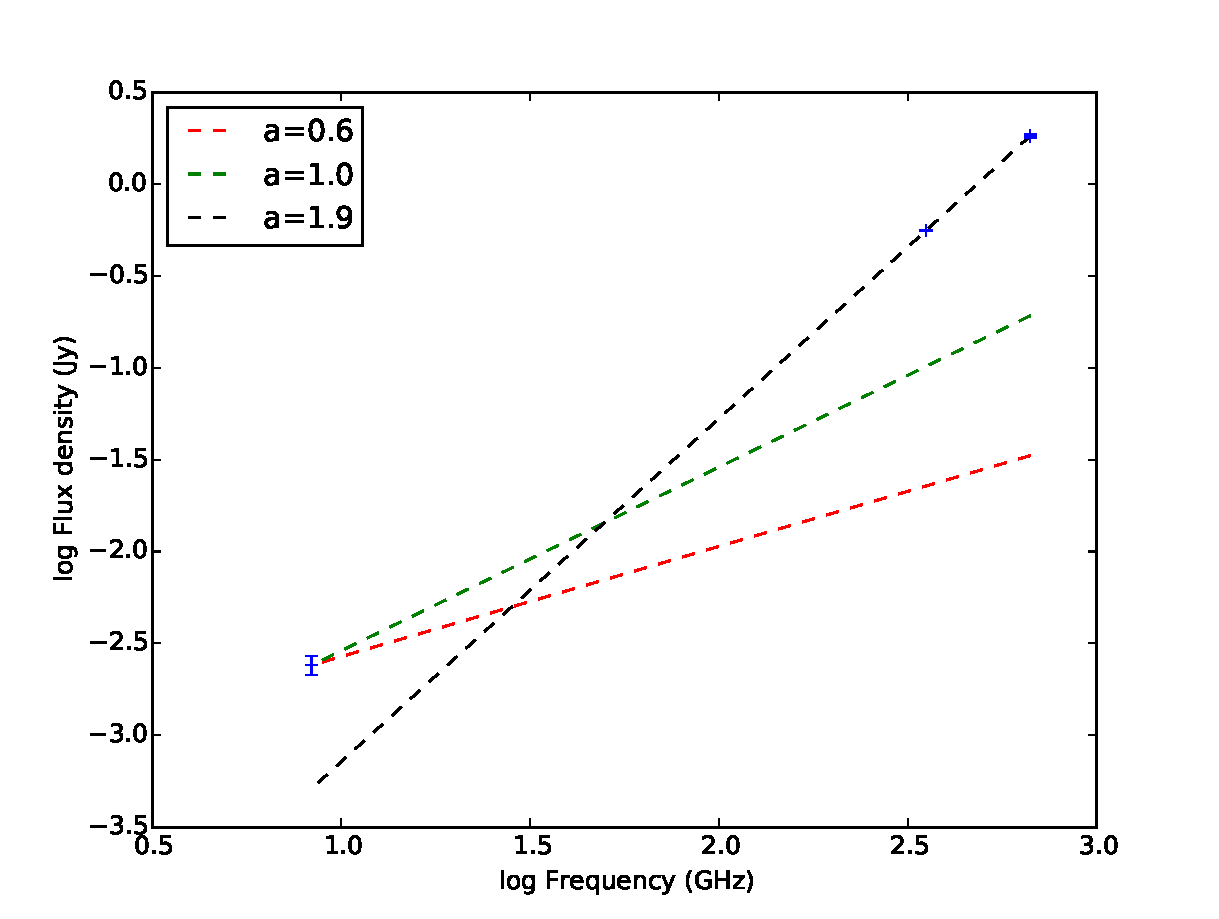
\includegraphics[scale=0.5]{c4/figs/ffOS2a.pdf}
%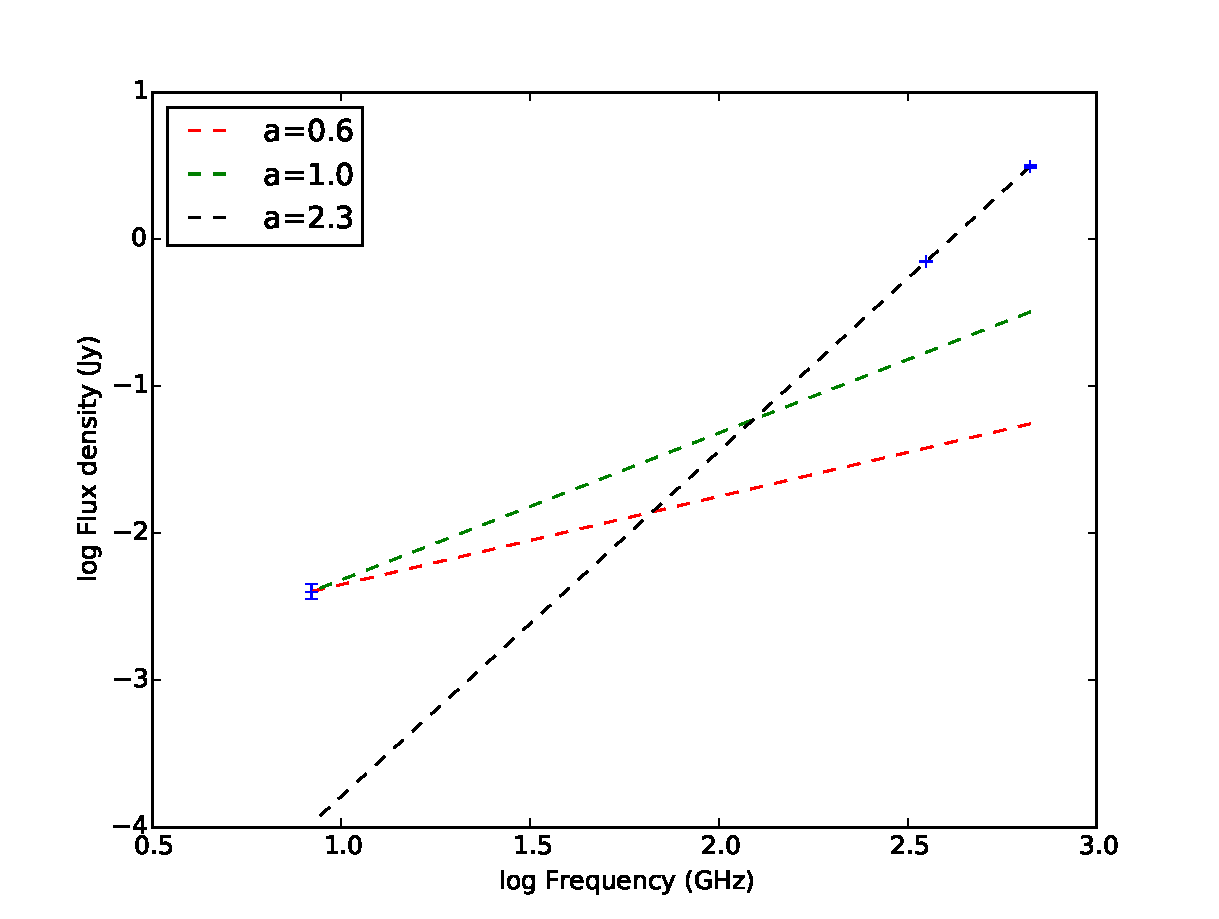
\includegraphics[scale=0.35]{c4/figs/ffOS2b.pdf}
\end{tabular}
\caption{Modelling free-free emission in OS2a from the Rodriguez et al. (2010) 3.6\,cm data for a given $\alpha_{\mathrm{ff}}$ = 0.6 (red), 1.0 (green), and the observed dust spectral index (black).} 
\label{fig:freefreemodel}
\end{centering}
\end{figure*} 

%W40 - OS1 
OS1 is a close cluster of objects that are not resolved by SCUBA-2 or the AUI/NRAO beam but are listed as a number of objects in \cite{Rodriguez:2010bs}, four of which have none-variable emission indicating an \UCHII\ region. There is also no significant emission at 450\,$\micron$ which suggests that if there is any free-free contribution at 850\,$\micron$, the emission has become optically thin by 450\,$\micron$. An $\alpha_{\mathrm{ff}}$ = 0.6 represents emission of 6.36\,mJy of free-free at 850$\micron$, a 50\% contribution. This result is consistent with the presence of HAeBe stars in the cluster. No jet shocks are found in the vicinity of the cluster and so we rule out the collimated jet configuration of free-free emission.

%W40 - OS2a
OS2a is a single HAeBe star that is resolved as a strong point source by SCUBA-2 at both 450\,$\micron$ and 850\,$\micron$. \cite{Rodriguez:2010bs} does resolve both OS2a at 3.6\,cm and therefore these fluxes are used to complete the contribution test. Two results are returned; an $\alpha_{\mathrm{ff}}$ = 0.6 represents a 5\% contribution (1.86\,mJy) and an $\alpha_{\mathrm{ff}}$ = 1.0 represents a 22\% contribution (8.18\,mJy). 
%W40 -EDIT
OS2a is variable in nature but it also has nearby shock fronts which are consistent with active accretion, so the jet scenario of $\alpha_{\mathrm{ff}}$ = 1.0 appears the more likely outcome. No spectral class is available for this object. 
Both tests infer that even if the free-free emission is opaque at SCUBA-2 wavelengths, the SCUBA-2 source is remains dominated by dust emission. These results, and others, are summarised in Table \ref{tab:stars}.
%NEW - OS2b
OS2b has a SCUBA-2 peak at both wavelengths but given its spectral class of B4 we consider it unlikely that any free-free emission will remain optically thick in the submillimetre regime. 

%W40 - VLA peaks
In addition to this radio catalogue, we identify four radio peaks in Archival AUI/NRAO 3.6\,cm map which were outside 
of the coverage of \cite{Rodriguez:2010bs} which are marked in Figure \ref{fig:3_6cm} as VLAa, b, c and d. As there is no clear point source in the SCUBA-2 maps we assume that these additional VLA radio sources are optically thin at these wavelengths and take no further action.






\section{The free-free contribution in Serpens MWC 297 results and discussion.}

%NEW
\begin{table}%[h]
\caption{Summary of free-free contributions to SCUBA-2 wavelengths from MWC 297. The uncertainty on flux density at 450\,$\micron$ is 0.03\,Jy and 850\,$\micron$ is 0.0025\,Jy. }
\begin{tabular}{@{}|c|ccccccccc|c|}
       & 3.6\,cm (Jy)	& \multicolumn{4}{c}{450\,$\micron$ (Jy)} & \multicolumn{4}{c}{850\,$\micron$ (Jy)} \\
Object &	VLA$^{a}$	& SCUBA-2       & Free-free      & Dust      & \%      & SCUBA-2      & Free-free      & Dust       & \% 	& $\alpha_{\mathrm{ff}}$     \\
\hline
\hline
MWC 297   &	0.0099	& 0.1886             &  0.1377         &  0.0510 & 73$\pm$5 & 0.0860	&	0.0709	&	0.0150	&	82$\pm$4	&	1.03      \\

\hline
\end{tabular}\\
\raggedright

\label{tab:MWC297}
\end{table}

%MWC 297 - critique free-free nature
We determine that free-free emission from an UCH\textrm{II} region and polar jets/winds associated with MWC 297 contaminates the 450\,$\micron$ and 850\,$\micron$ data \citep{Skinner:1993bh}. The nature of the free-free emission from the outflow has been debated by various authors. \cite{Malbet:2007zr} and \cite{Manoj:2007ly} argue for ionised stellar winds that dominate at higher latitudes, whereas \cite{Skinner:1993bh} and \cite{Sandell:2011dz} provide evidence for an additional source of free-free emission in the form of highly collimated polar jets. Jets are typically associated with less evolved objects where luminosity is dominated by accretion processes whereas MWC 297 is considered to be a Class III / ZAMS star where the majority of the disk has fallen onto the star or been dissipated by winds. 

%MWC 297 - Xray flares - companion 
X-ray flares are thought to be a signature of episodic accretion and \cite{Damiani:2006ve} detect a number of X-rays flares from the Serpens MWC 297 region but find that only 5.5\,per cent of total flaring is directly associated with MWC 297, suggesting that accretion onto it is minimal. The majority of X-ray emission is associated with additional YSOs and the companion of MWC 297, \emph{OSCA}, an A2V star identified by \cite{Habart:2003fk} and \cite{Vink:2005uq} at a separation of 850\,AU. 

%MWC 297 - EDIT- flux results
Figure~\ref{fig:freefreeSED} and Figure~\ref{fig:contamination} show that free-free emission due to an UCH\textrm{II} region and polar winds/jets is responsible for the majority of flux from the star MWC 297. Original peak fluxes of 188$\pm$16\,mJy and 86$\pm$22\,mJy. Residual dust peak fluxes are $51\pm10$ mJy and $15\pm3$ mJy flux per pixel at 450\,$\micron$ and 850\,$\micron$ respectively and are highlighted in Figure~\ref{fig:freefreeSED} as the flux above the free-free power law fit of $\alpha = 1.03\pm0.02$. Free-free subtraction increases the residual dust spectral index by 35\%. This corresponds to approximately 73$\pm$5\,per cent and 82$\pm$4\,per cent of the 450\,$\micron$ and 850\,$\micron$ peak flux respectively. Given our estimate of 13\,per cent CO contamination, dust emission could potentially account for as little as 5\,per cent of peak emission at 850\,$\micron$. 

%MWC 297 - dust in MWC 297?
The 5$\sigma$ level of 82\,mJy and 11\,mJy means that flux is too uncertain to be detected at 450$\micron$ and therefore it is not possible to calculate reliable temperatures of the residual circumstellar envelope/disk around the star. The assumption of point-like free-free emission may add further uncertainty to the residual flux. We cannot say whether any dust emission contributes at the position of MWC 297. 

\section{The free-free contribution in the W40 complex results and discussion.}

%W40
\begin{table}%[h]
\caption{Summary of free-free contributions to SCUBA-2 wavelengths from bright objects in W40. The uncertainty on flux density at 450\,$\micron$ is 0.017\,Jy and 850\,$\micron$ is 0.0025\,Jy. }
\begin{tabular}{@{}|c|ccccccccc|c|}
       & 3.6\,cm (Jy)	& \multicolumn{4}{c}{450\,$\micron$ (Jy)} & \multicolumn{4}{c}{850\,$\micron$ (Jy)} \\
Object &	VLA$^{a}$	& SCUBA-2       & Free-free      & Dust      & \%      & SCUBA-2      & Free-free      & Dust       & \% 	& $\alpha_{\mathrm{ff}}$     \\
\hline
\hline
OS1$^{b}$   &	0.00578	& -             & -              & -         & -       & 0.101        & 0.064          & 0.038      & 62	&	0.6      \\
OS2a   &	0.00240	& 1.83          & 0.16           & 1.67      & 9      & 0.558        & 0.069          & 0.489      & 12	&	1.0     \\
\hline
\end{tabular}\\
\raggedright
$^{a}$ VLA 3.6\,cm compact object fluxes \citep{Rodriguez:2010bs}. \\
$^{b}$ OS1 covers a cluster for stellar objects where OS1a(North), VLA-12, VLA-14, VLA-16 are all radio emitters. The flux of the most prominent source, VLA-14, is included in this table but in reality the SCUBA-2 free-free flux of OS1 is a combination of all 4 of these objects. \\
\label{tab:freefree}
\end{table}

%NEW - preamble
The W40 complex contains a number of massive stars that are detected in high resolution VLA 3.6\,cm observations. A large-scale \HII\ region is also observed at lower resolution 21\,cm observations. 

%W40 - EDIT - large-scale results
Figure \ref{fig:freefree21} shows how the SCUBA-2 data is subsequently aligned and convolved to the larger resolution of the VLA 21\,cm data so the two data sets are directly comparable. Given that free-free emission from the large scale \HII\ region is essentially flat in spectrum, it is not surprising that the contribution is very limited. Peak 21\,cm flux density is 0.0298\,Jy/pix which corresponds to 0.0163 and 0.0174\,Jy/pix at 450 and 850\,$\micron$ given a spectral index of 
$\alpha_{\mathrm{ff}}$ = -0.1. The contribution of this peak flux to the SCUBA-2 observations is 5\% at 850\,$\micron$ and 0.5\% at 450\,$\micron$. 
%NEW
As a result the dust spectral index for the peak increases by 2\% from 3.46 to 3.53.

%W40 - EDIT - small scale results
3.6\,cm fluxes for OS1 and OS2a are extrapolated up to SCUBA-2 wavelengths (Table \ref{tab:freefree}) assuming an indirectly estimated free-free spectral index of 0.6 and 1.0 respectively. Modelled as a point source, the free-free emission from each star is convolved with the JCMT beam using primary and secondary components for comparison with the SCUBA-2 data (Figure \ref{fig:freefree3_6}). The contribution of the free-free in OS1a at 850\,$\micron$ 
is 62\% (no detection at 450\,$\micron$). The free-free contribution for OS2a is 9\% at 450\,$\micron$ and 
12\% at 850\,$\micron$. 
%NEW
As a result the dust spectral index for the peak increases by 3\%.

%NEW - OS2b alpha
Having accounted for possible CO and free-free contamination, the residual flux detected from OS2a is 1.67 and 0.489\,Jy at 450\,$\micron$ and 850\,$\micron$ respectively. We find that this gives OS2a an usually low spectral index of 1.6$\pm$0.1. 
%W40
Whilst lower $\alpha$s have previous been explained by very low $\beta$ associated with grain growth \citep{Manoj:2007ly}, given a $\beta$=1.0, typical for circumstellar disks, an $\alpha$ = 1.6 would require a temperature of less than 2\,K. Alternatively, an exceptionally low $\beta$ approaching 0.0 would still require a temperature of less than 7\,K. In both scenarios, dust temperatures this low have never been observed. Therefore the results calculated for OS2a should be considered with a high degree of scepticism.


%W40 - summary contamination
In summary, the free-free contribution at SCUBA-2 wavelengths is limited (less that 5\%) at large 
scales. At smaller scales it may have a small, but significant (9\% to 12\%) impact on prominent 
SCUBA-2 sources such as OS2a and a significant impact (62\%) on faint SCUBA-2 sources such 
as OS1a. 
%NEW
Subtraction of the free-free emission from SCUBA-2 observations acts to increase the dust spectral index, by 2\% at the  peak of large-scale emission and 3\% from OS2b. 



\section{Conclusions}
%NEW
In this chapter we have examined the impact of free-free contamination on SCUBA-2 observations of star-forming regions of Serpens MWC 297 and the W40 complex. We find a small number of cases in the literature where radio-bright YSOs have free-free emission that is optically thick at submillimetre wavelengths and contributes to SCUBA and SCUBA-2 observations in addition to dust. We develop techniques that are used to subtract this small scale emission from the submillimetre observations and measure the residual dust flux and estimate the contamination fraction. Where insufficient radio observations exist to directly calculate $\alpha_{\mathrm{ff}}$ we asses the physical characteristics of individual sources to make a judgement on wether they are \UCHII\ regions ($\alpha_{\mathrm{ff}}$ = 0.6) or collimated jets ($\alpha_{\mathrm{ff}}$ = 1.0). We also apply the same method to large scale, diffuse \HII\ regions with an  $\alpha_{\mathrm{ff}}$ = -0.1 to investigate.

Our results are summarised as:

\begin{enumerate}
\item The B1.5ve Herbig HAeBe star MWC 297 in the Serpens MWC 297 region has a free-free spectral index of $\alpha_{\mathrm{ff}}$ = 1.03$\pm$0.02, consistent with collimate jet geometry. SCUBA-2 peak fluxes of 188$\pm$16\,mJy and 86$\pm$22\,mJy are consistent with an outstanding point source at the location of MWC 297 inferring that free-free emission from the ZAMS-star maybe optically thick at submillimetre wavelengths.
\item Free-free emission from MWC 297 was found to contribute to approximately 73$\pm$5 per cent and 82$\pm$4 per cent of the 450\,$\micron$ and 850\,$\micron$ peak flux respectively. Residual dust peak fluxes are 51$\pm$10\,mJy and 15$\pm$3\,mJy flux per pixel at 450\,$\micron$ and 850\,$\micron$ respectively. Subtracting the free-free emission increases the spectral dust index by 35\%. Dust at 850\,$\micron$ represents a 1.4$\sigma$ detection and at 450\,$\micron$ a 0.6$\sigma$ detection confirming that any residual disc around MWC 297 is too faint to be reliably detected. 
\item A number of radio bright stars are observed in the W40 complex in the IR. OS1b, c, OS3a and IRS 5 are not detected in SCUBA-2, confirming that any free-free emission from these objects is optically thin at submillimetre wavelengths and no contamination subtraction is required.
\item The O9.5 MS-star OS1a and a cluster members VLA 12, 14 and 15 are non-variable compact radio sources with no evidence jet features observed. We classify these as \UCHII\ regions with $\alpha_{\mathrm{ff}}$ = 0.6 and calculate a free-free contribution of 62\% at 850\,$\micron$ (no detection at 450\,$\micron$).
\item The Herbig AeBe star OS2a has a variable compact radio source consistent with episodic accretion. Radio shock fronts are also observed in the vicinity that would be consistent with jet emission. A significant SCUBA-2 peak of 1.83 and 0.558\,Jy at 450\,$\micron$ and 850\,$\micron$ respectively is associated with this object. We classify this object as a collimated jet with an $\alpha_{\mathrm{ff}}$ = 1.0 and calculate a free-free contribution of 9\% at 450\,$\micron$ and 12\% at 850\,$\micron$. Subtracting the free-free emission increases the spectral dust index by 2\%. The residual dust has an unusually low spectral index 1.6$\pm$0.1 which is is difficult to explain without invoking exceptional cold dust temperatures. 
\item The B4 star OS2b has a variable compact radio source consistent with episodic accretion but lacks any signatures of jet emission. If a weak \UCHII\ region is being detected it would be consistent with the B4 spectral class of the star which lies right on the threshold of sufficient Lyman photon production to power an \HII\ region. We therefore judge that any free-free emission from this star would optically thin at SCUBA-2 wavelengths. 
\item The large, diffuse \HII\ region is observed in the W40 complex. This feature has an $\alpha_{\mathrm{ff}}$ = -0.1 and has a peak flux of 0.03\,Jy/pix in 21\,cm VLA data which has a free-free contribution of 0.5\% at 450\,$\micron$ and 5\% at 850\,$\micron$. Subtracting the free-free emission increases the spectral dust index by 3\%.

Our results lead us to believe that where free-free emission is sufficiently bright and optically thick its contribution can lead to the observation of prominent point sources and significantly lower dust spectral indices, and therefore temperatures. Where the free-free emission is less prominent, in faint \UCHII\ regions and from large-scale \HII\ it can still have a limited, if non-negligible impact on the dust spectral index. In the following chapter we will look at what quantifiable affects the free-free emission has when examining the dust temperature.



 
   
   % Temperate mapping
   \chapter{Temperature mapping}
\label{ch:chapter5}

\section{Introduction to the temperature equation}
\subsection{Submillimetre Flux ratio}
%MWC 297
Using the ratio of 450\,$\micron$ and 850\,$\micron$ fluxes from SCUBA-2, 
we develop a method that utilises the two frequency observations of the same 
region where the ratio depends partly on the dust temperature ($T_{\mathrm{d}}$) 
via the Planck function and also on the dust opacity spectral index, $\beta$ 
(a dimensionless term dependent on the grain model as proposed by 
\citeauthor{Hildebrand:1983fy}\,\citeyear{Hildebrand:1983fy}), as described by 
\begin{equation}
\frac{S_{\mathrm{450}}}{S_{\mathrm{850}}} = \left ( \frac{850}{450} \right )^{3+\beta }\left ( \frac{\exp(hc/\lambda _{\mathrm{850}}k_{\mathrm{B}}T_{\mathrm{d}})-1}{\exp(hc/\lambda _{\mathrm{450}}k_{\mathrm{B}}T_{\mathrm{d}})-1} \right ), \label{eqn:temp}
\end{equation}
otherwise referred to as `the temperature equation' \citep{Reid:2005ly}.
%MWC 297
There is no analytical solution for temperature and so pixel values are inferred from 
a lookup table. The method by which temperature maps are made can be split into 
two distinct parts: creating maps of flux ratio from input 450\,$\micron$ and 850\,$\micron$ 
data and building temperature maps based on the ratio maps. Both methods were 
discussed by \cite{Hatchell:2013ij}, for here on referred to as the H13 method. 
We focus on the development of this method and the additional features that have 
been incorporated.

\subsection{Beta}
%MWC 297
\begin{figure}
\begin{centering}
\includegraphics[scale=0.35]{/Users/damian/Documents/Thesis_et_al/images/20131228_FluxRatio.pdf}
\caption{Flux ratio as a function of temperature as described by Equation \ref{eqn:temp}. The temperature range is that commonly observed in protostellar cores.} \label{fig:SR_temp}
\end{centering}
\end{figure} 
%MWC 297
Temperature is known to influence the process by which dust grains coagulate 
and form icy mantles and therefore the value of $\beta$. Observations by 
\cite{Ubach:2012fk} have shown decreases in $\beta$ in protoplanetary disks 
but for the most part there is little evidence that $\beta$ changes significantly in 
pre/protostellar cores \citep{Schnee:2014uq}. \cite{Sadavoy:2013qf} fitted 
\emph{Herschel} 160\,$\micron$ to 500\,$\micron$ data with SCUBA-2 data in 
the Perseus B1 region  and concluded that $\beta$ is approximately 2.0 in 
extended, filamentary regions whereas it takes a lower value of approximately 
1.6 towards dense protostellar cores. 
%MWC 297
Figure~\ref{fig:SR_temp} describes how small changes in $\beta$ lead to a 
large range of flux ratios, especially at higher temperatures. For ratios of 3, 7 
and 9, a $\beta$ of 1.6 would return temperatures of 8.9, 25.4 and 85\,K whereas 
a $\beta$ of 2.0 would return temperatures of 7.6, 15.7 and 25\,K. Higher ratios 
indicate heating above that available from the Interstellar Radiation Field (ISRF) 
for any reasonable value of $\beta$. 
%MWC 297
Removing the requirement for the uncertainty in $\beta$ requires data at additional 
wavelengths, for example 250\,$\micron$ and 350\,$\micron$ as observed by 
\emph{Herschel}. Reconciling the angular scales of \emph{Herschel} observations 
with those of SCUBA-2 is a non-trivial process and goes beyond the scope of this paper. 
%MWC 297
Smaller values of $\beta$ are found to be consistent with grain growth which only 
occurs sufficiently close to compact structures \citep{Ossenkopf:1994vn}. 
\cite{Stutz:2010hq} used the dominance of extended structure to that of compact 
structure to argue for a uniform, higher value of $\beta$. Likewise \cite{Hatchell:2013ij} 
assumed a constant $\beta$, arguing that variation in temperature dominates to that 
of $\beta$ in NGC1333. On this basis we adopt a uniform $\beta$ of 1.8, a value 
consistent with the popular OH5 dust model proposed by \cite{Ossenkopf:1994vn} 
and studies of dense cores with \emph{Planck}, \emph{Herschel} and SCUBA-2 
\citep{Stutz:2010hq, Juvela:2011ys, Sadavoy:2013qf}. We note that in this regime an 
apparent fall in temperature towards the centre of a core might be symptomatic of 
low $\beta$ values and therefore we cannot be as certain about the temperatures 
at these points.


\subsection{Alpha}
\subsection{Temperature}



\section{Dual beam method}
\subsection{The JCMT beam (primary and secondary)}

%FROM MWC 297
The JCMT beam can be modelled as two Gaussian components \citep{Drabek:2012uq, 
Dempsey:2013uq}. The primary (or main) beam contains the bulk of the signal and is 
well described by a Gaussian, $G_{\mathrm{MB}}$, but in addition to this there is also 
a secondary beam which is much wider and lower in amplitude, $G_{\mathrm{SB}}$. 
Together they make up the 2-component beam of the telescope, 
%FROM MWC 297
\begin{equation}
G_{\mathrm{total}}=a G_{\mathrm{MB}} + b G_{\mathrm{SB}}, \label{eqn:effbeam} 
\end{equation}
where $a$ and $b$ are relative amplitude, listed in Table~\ref{table:beams} 
alongside the FWHM, $\theta$, of the primary (MB) and secondary (SB) beams.   
%FROM MWC 297
%\begin{table}
%\caption{JCMT beam properties}
%\label{table:beams}
%\begin{center}
%\centering
%\begin{tabular}{l | p{1cm} | p{1cm}  }
%		&	450\,$\micron$ &	850\,$\micron$ \\
%	\hline
%	$\theta_{\mathrm{MB}}$ &	7.9\arcsec\	&	13.0\arcsec\		\\
%	$\theta_{\mathrm{SB}}$	&	25.0\arcsec\	&	48.0\arcsec\		\\	
%	$a$	&	0.94	&	0.98		\\
%	$b$	&	0.06	&	0.02		\\
%	Pixel size&	4\arcsec\	&	6\arcsec\		\\
%	\hline
%\end{tabular}
%\end{center}
%JCMT beam Full Width Half Maximum ($\theta$) and relative amplitudes from \cite{Dempsey:2013uq} Table 1. Pixel sizes are those chosen by the JCMT SGBS data reduction team.

\subsection{Gaussian beam convolution}
%MWC 297
We introduce a secondary beam component into the H13 method, which previously 
assumed that the secondary component was negligible. This adds complexity 
to the convolution process as it requires convolution of the data with a normalised 
Gaussian of the form of the JCMT beam's primary and secondary components for 
the alternative wavelength. The primary component at 850\,\micron\ is then scaled with 
%MWC 297
\begin{equation}
\frac{a_{\mathrm{450}}\theta _{\mathrm{MB_{\mathrm{450}}}}^{2}}{a _{\mathrm{450}}\theta _{\mathrm{MB_{\mathrm{450}}}}^{2}+b _{\mathrm{450}}\theta _{\mathrm{SB_{\mathrm{450}}}}^{2}}, \label{eqn:scaleMB}
\end{equation}
%MWC 297
and likewise 
%MWC 297
\begin{equation}
\frac{b_{\mathrm{450}}\theta _{\mathrm{SB_{\mathrm{450}}}}^{2}}{a_{\mathrm{450}}\theta _{\mathrm{MB_{\mathrm{450}}}}^{2}+b_{\mathrm{450}}\theta _{\mathrm{SB_{\mathrm{450}}}}^{2}}, \label{eqn:scaleSB}
\end{equation} 
for the secondary component. The 450\,$\micron$ map is convolved with the 850\,$\micron$ 
beam is a similar way. Corresponding parts are then summed together for 450\,$\micron$ and 
850\,$\micron$ data separately to construct the convolved maps with an effective beam size of 
19.9\arcsec\ as shown in Figure~\ref{fig:mwc}.


\subsection{4 component dual beam convolution method}
%MWC 297
\begin{figure(}
\begin{center}
\includegraphics[scale=0.5]{/Users/damian/Documents/Thesis_et_al/images/temp_flowchart_simple.pdf}
\caption{A flow chart providing a simplified description of the ratio mapping process}
\label{fig:flow}
\end{center}
\end{figure*}

%MWC 297
Free parameters of our method are limited to $\beta$ (which we set at 1.8). Input 
450\,$\micron$ and 850\,$\micron$ flux density data (scaled in Jy/pixel) have fixed 
noise levels. Other fixed parameters which are used in the beam convolution 
include: the pixel area per  map, FWHM of the primary ($\theta_{\mathrm{MB}}$) 
and secondary ($\theta_{\mathrm{SB}}$) beams and beam amplitudes all of which 
are measured by \cite{Dempsey:2013uq} and given in Table \ref{table:beams}.
%MWC 297
Input maps are first convolved with the JCMT beam (Equation 1) at the alternate 
wavelength to match resolution. Pixel size is taken into account in this process.
The 450\,$\micron$ fluxes are then regridded onto the 850\,$\micron$ pixel grid. 
Data are then masked leaving only 5$\sigma$ detections or higher. 450\,$\micron$ 
fluxes are then divided by 850\,$\micron$ fluxes to create a map of flux ratio.
%MWC 297
Whereas the H13 method made a noise cut based on the variance array calculated 
during data reduction, our model introduces a cut based on a single noise estimate, 
following the method introduced by \cite{Salji:2013kx}. The data are masked to remove 
pixels which carry astronomical signal. The remaining pixels are placed in a histogram 
of intensity and a Gaussian is fitted to the distribution, from which a standard deviation, 
$\sigma$,  can be extracted as the noise level. This calculation is a robust form of 
measuring statistical noise that includes residual sky fluctuations.
%MWC 297
%TJW calculated flux in units per beam beam which necessititated a calibration factor and an associated error of 5 to 10per cent depending on wavelength \citep{Dempsey:2013uq} however since then GBS Internal Release 1 standard has revised the units of input data array to units per pixel which eliminates this necessary calbriation and source of statisical error. As a result the improved error derived from the noise level can be propagated through the various process with the model to produce new error arrays. 
%MWC 297
The inclusion of the secondary beam was found to decrease temperatures by between 5 per cent and 
9 per cent with the coldest regions experiencing the largest drop in temperature and warmest the least. 
%MWC 297
Applying a 5$\sigma$ cut based on the original 450\,$\micron$ data to mask uncertain regions of 
large scale structure after the beam convolution can lead to spuriously high values around the 
edges of our maps where fluxes from pixels below the threshold are contributing to those above, 
producing false positives. These `edge effects' are mitigated by clipping but we advise that 
where the highest temperature pixels meet the map edges these data be regarded with a degree of scepticism. 
%MWC 297
%Our model produces more reliable temperatures as a result of using the full beam whereas 
%the H13 method does not. For point sources, such as YSOs and prestellar cores, our results 
%show that the effect of the secondary beam is non-negligible, having an ameliorating effect 
%on ratio and temperature. Flux from individual pixels is spread out over a wider area through 
%convolution. At the 5$\sigma$ noise level we observe how unreliable data can encroach on 
%reliable data and produce artefacts known as `edge effects'. The offset in values of $\alpha$ 
%and $\beta$ between 450\,$\micron$ and 850\,$\micron$ listed in Table~\ref{table:beams} 
%produces contrasting beam profiles. Where underlying large scale structure encroaches on 
%significant data, we see a substantial divergence in fluxes in favour of exceptionally larger flux 
%ratios, resulting unrealistically high temperatures in these regions. 
%MWC 297
%the impact of these artefacts can be reduced through careful clipping of the data. Large scale structure regions 
%are inherently less dense than point-like dense cores and therefore often fall bellow the 5$\sigma$ noise level 
%and are cut from the maps. As these regions do not hold significant observations, it is not a concern that they 
%also contain artefacts. We cannot rule out all instances with this method as much of the SCUBA-2 data covers regions 
%of significant large-scale star-forming clouds. We cannot further adapt our processes to mitigate these effects, 
%however as this paper mainly studies YSOs which are point-like, the effect of these artefacts are unlikely to encroach 
%in these cases and we proceed with the proviso that a degree of scepticism should be cast towards 
%high temperature data on the edges of large scale regions. 
%MWC 297
Ratio maps are converted to temperature maps using Equation \ref{eqn:temp} 
implemented as a look-up table as there is no analytical solution. The H13 method 
subsequently cuts pixels with an arbitrary uncertainty in temperature of greater 
than 5.5\,K. We replace this with a cut of pixels of an uncertainty in temperature 
(calculated from the noise level propagated through the method described in 
Section 3.1) of greater than 5 per cent. 

\section{Propagation of error}
\subsection{Analytical calculation}
\subsection{Monte-Carlo method}
\section{Testing Dual beam method}
\section{Kernel method}
\subsection{Convolution kernel}
\subsection{Beam model/beam map}
\subsection{Preparing the Kernel}
\section{Propagation of error}
\subsection{Monte-Carlo method}
\section{Testing Kernel method}
\subsection{Pixel size problem}
\section{Comparing ratio methods}
\section{Calculating temperature}
\subsection{Edge effects}
\subsection{Comparison with alternative methods}
\section{The impact of CO contamination}
\section{The impact of the free-free contribution}
%MWC297
\begin{figure*}
\begin{center}
\includegraphics[scale=0.7]{20140718_MWC297_tempcomp.jpeg}
\caption{Temperature maps of MWC 297 from the ratio of 450\,$\micron$ and 850\,$\micron$ emission pre (\emph{left}) and post (\emph{right}) free-free 
contamination subtraction. Contours are at 11, 25 and 38\,K. The location of MWC 297 is marked with a star.}
\label{fig:Tcomp}
\end{center}
\end{figure*}
%MWC297
Figure~\ref{fig:contamination} presents the 850\,$\micron$ before and after subtraction. Figure~\ref{fig:Tcomp} presents the impact of free-free emission on temperature maps of the region. Even with the free-free emission subtracted, a large, extended submillimetre clump remains, though its peak is offset from the location of MWC 297 by 24.2\arcsec\ (approximately 6,000\,AU).
%MWC 297
The impact of this contamination on the temperature maps is remarkable. The power law of $\alpha = 1.03\pm0.02$ that describes free-free emission from both an UCH\textrm{II} region and jet outflows produces greater flux at 850\,$\micron$ than 450\,$\micron$. Free-free dominates the flux and this results in artificially lower ratios and therefore lower temperatures. This is consistent with the cold spot seen in Figure \ref{fig:Tcomp}a at the location of the UCH\textrm{II} region, with a temperature of approximately 11\,K. We can conclude that free-free emission may contaminate submillimetre temperature maps where cold spots are coincident with hot OB stars.
%MWC 297
The 5$\sigma$ level of 82\,mJy and 11\,mJy means that flux is too uncertain to be detected at 450$\micron$ and therefore it is not possible to calculate reliable temperatures of the residual circumstellar envelope/disk around the star. 
%MWC297
\begin{figure*}
\begin{center}
\includegraphics[scale=0.7]{/Users/damian/Documents/Thesis_et_al/images/20140718_MWC297_tempcomp.pdf}
\caption{Temperature maps of MWC 297 from the ratio of 450\,$\micron$ and 850\,$\micron$ emission pre (\emph{left}) and post (\emph{right}) free-free 
contamination subtraction. Contours are at 11, 25 and 38\,K. The location of MWC 297 is marked with a star.}
\label{fig:Tcomp}
\end{center}
\end{figure*}
%MWC 297
\begin{figure*}
\begin{center}
\includegraphics[scale=0.7]{/Users/damian/Documents/Thesis_et_al/images/20140618_mwc297_contamination.pdf}
\caption{IR1 SCUBA-2 850\,$\micron$ data before \emph{left} and after \emph{right} removal of free-free contamination from an UCH\textrm{II} region and polar jets/winds (represented by the point source contours in the \emph{left} plot). SCUBA-2 contours are at 0.011, 0.022, 0.033 and 0.055 Jy/pixel (corresponding to 5, 10, 15 and 25 $\sigma$ detection limits). 6\,cm VLA contours (red) from Sandell (private comm.) at 0.002, 0.005, 0.02, 0.072, 0.083 Jy/beam are overlaid on the left hand panel. The location of MWC 297 is marked with a star. Beam sizes are shown at the bottom of the image (VLA CnD config. \emph{left} and JCMT \emph{right}.) }
\label{fig:contamination}
\end{center}
\end{figure*}


 
   
   % Radiative heating in Serpens MWC 297 region
   \chapter{Radiative heating in Serpens MWC 297 region}
\label{ch:chapter6}


\section{Temperature maps of Serpens MWC 297}

%MWC 297
\begin{figure*}
\begin{center}
\includegraphics[scale=0.7]{/Users/damian/Documents/Thesis_et_al/images/20140820_MWC297_tri_panel.pdf}
\caption{Top to bottom: a) SCUBA-2 convolved 850\,$\micron$ flux map of Serpens MWC 297. Contours from the original 850\,$\micron$ data are at 0.011, 0.033\,Jy/pixel (corresponding to 5 and 15 $\sigma$). b) SCUBA-2 convolved and aligned 450\,$\micron$ flux map of Serpens MWC 297 in Jy/pixel. Contours from the original 450\,$\micron$ data are at 0.082, 0.25\,Jy/pixel (corresponding to 5 and 15 $\sigma$). The crosses in a) and b) mark the location of the ZAMS B1.5Ve star MWC 297 and its binary partner \emph{OSCA} (A2v). c) Dust temperature map of Serpens MWC 297 for $\beta$ = 1.8. Contours of \emph{Spitzer} 24\,$\micron$ emission at 32, 40 and 70\,MJy per Sr are overlaid.}
\label{fig:mwc}
\end{center}
\end{figure*}


The 450\,$\micron$ and 850\,$\micron$ SCUBA-2 data for the MWC 297 region are 
presented in Figure~\ref{fig:mwc} alongside a map of temperature of submillimetre 
dust in that region. These maps show a large diversity in temperature across five 
isolated regions of significant flux (shown in Figure~\ref{fig:mwc}c). Mean cloud 
temperatures range from 10.1$\pm$0.9\,K and 15$\pm$2\,K for regions which are 
relatively cold and isotropic, to 25$\pm$17\,K for warmer regions with a large diversity 
of temperatures. Figure~\ref{fig:Tcomp} shows one cloud that has a temperature of 41$\pm$19\,K 
which is hot to the extent that this would suggest an active heat source. The range in 
temperatures suggests that the regions within the Serpens MWC 297 vary in physical 
conditions. 

\cite{Menshchikov:2010kl} infer temperature variation from contrasting strengths of 
350\,$\micron$ flux bands to the shorter 70\,$\micron$ and 160\,$\micron$ 
bands of \emph{Herschel}. They quote a temperature range for dense, starless filaments 
of 7.5 to 15\,K across the whole Aquila rift. However, we do not observe a typical filamentary 
structure in Serpens MWC 297 region (Figure \ref{fig:maps}).

\cite{Konyves:2010oq} and \cite{Bontemps:2010fk} used single-temperature modified black-body 
fitting of SEDs of \emph{Herschel} 500\,$\micron$ data points in Aquila and Polaris. 
Their study includes Serpens MWC 297 and they find temperatures for the 
region ranging between 24 and 26\,K. Though \emph{Herschel} 500\,$\micron$ data is 
at a lower resolution than our effective beam, the general temperatures of the region seem 
consistent with our findings. 

\cite{Hatchell:2013ij} use only the primary beam to study NGC1333, finding typical dust temperatures 
of ranging from 12 to 16\,K. They also argue for a heated region pushing temperatures up as 
high as 35 to 40\,K near the location of the B star SVS3. When the moderating effects of the 
secondary beam are taken into account, these results are largely consistent with our findings 
(Serpens MWC 297 also contains a B star). 

Figure~\ref{fig:mwc}c shows \emph{Spitzer} MIPS 24\,$\micron$ flux for the Serpens MWC 297 
region. These data show hot compact sources associated with individual stellar cores. It also 
shows the morphology of an extended IR nebulosity, associated with SH2-62, that is centred 
on MWC 297. As well as the dust within the immediate vicinity of the star MWC 297 showing clear 
signs of heating, we observe 24\,$\micron$ emission that is coincident with heating in the SCUBA-2 
temperature maps. As 24\,$\micron$ emission provides independent 
evidence of heating, where we observe high temperature pixels that are not coincident with 
24\,$\micron$ emission (for example in the northernmost cloud) we conclude we are likely 
witnessing data reduction artefacts as opposed to warm gas and dust. 

In addition to providing evidence for direct heating by MWC 297, the 24\,$\micron$ data also 
provide strong evidence that the B star is physically connected to the observed clouds. 
The Aquila rift is thought to be a distance of 250$\pm$50 pc \citep{Maury:2011ys} and through 
association we conclude that the distance to MWC 297 matches this figure.


\section{The SCUBA-2 clump catalogue}

In this section we introduce the clump-finding algorithm \textsc{fellwalker} used to identify 
clumps in the SCUBA-2 data presented in Figure~\ref{fig:maps}. We calculate clump 
masses and compare these to their Jeans masses to determine whether or not the objects 
are unstable to gravitational collapse. 

\subsection{Fellwalker parameters}


We tuned the \textsc{fellwalker} algorithm to produce a set of objects consistent 
with a by-eye decomposition, setting the following parameters; \emph{MinDip} 
= 1$\sigma$ (minimum flux between two peaks), \emph{MinPix} = 4 pixels (minimum number 
of pixels per valid clump), \emph{MaxJump} = 1 pixel (distance between clump 
peaks), \emph{FWHMBeam} = 0 (FWHM of instrument), \emph{MinHeight} = 3$\sigma$ 
(minimum height of clump peak to register as a valid clump) and \emph{Noise} = 3$\sigma$ 
(detection level). Throughout this process we used a constant noise level, 
$\sigma$, calculated via the method described by \cite{Salji:2013kx} and described in 
Section 3.1. \cite{watson:2010pc} discusses the \textsc{fellwalker} parameters in depth 
and concludes \emph{MinDip} and \emph{MaxPix} are the most influential in returning 
the maximum breakup of clouds into clumps, a subset of which will later be used to compile 
a list of protostellar cores. The $3\sigma$ level allows for the detection of the smallest 
clumps that may be missed at the $5\sigma$ level on account of insufficient pixels for 
detection as outlined above. This method also included a number of spurious clumps 
associated with high variance pixels at the maps edges. In order to avoid these we first 
masked the SCUBA-2 data with the data reduction mask shown in Figure \ref{fig:maps}. 

%We parameterise \textsc{fellwalker} to detect clumps consistent with 3$\sigma$ or greater 
%detections from 850\,$\micron$ data. The same boundaries are then used consistently 
%on the 450\,$\micron$ data. Spurious data around the edges of the map resulting from the 
%scanning procedure are removed. \cite{watson:2010pc} discusses the \textsc{fellwalker} 
%parameters in depth and concludes \emph{MinDip} and \emph{MaxPix} are the most 
%influential in returning the maximum number of clumps, and therefore identifying smaller scale 
%cores, and we set these equal to the $rms$ noise level and four pixels respectively. 
%We also found \emph{FWHMBeam} was important and setting this to zero included 
%all point sources regardless of size whereas setting \emph{MaxJump} to one pixel 
%isolated sources that were closer to each other. \emph{MinHeight} and \emph{Noise} 
%were both set to minimum statistical certainty of $3\sigma$,  \emph{MaxBad} was 
%set to 100 to stop pixels being eliminated if they were contact with `bad' data. 

Using these parameters 28 submillimetre clumps were detected in 850\,$\micron$ data 
and are presented in Figure \ref{fig:clumps}. Two sources (SMM 23 and 25) were immediately 
discarded as they were not consistent with a 5$\sigma$ detection. A further two clumps 
were split into two separate objects by the algorithm when there was no discernible peak 
in the submillimetre data. In these cases (SMM 7 \& 8 and SMM 13 \& 14) the objects were 
recombined into single object. We note that this is a side effect of having a low \emph{MinDip} 
parameter to maximise the detection of smaller clumps.  In total a sample of 23 clumps 
are presented in Table 3. We note that there is a known bias that underestimates the 
size of a clump as its peak flux approaches the cutoff level and therefore biases against 
the detection of cold, faint objects (examples might be SMM 26 and 27). Modelling 
clump profiles could be used to better estimate the full extent of these objects. However, 
as these present a minority of cases we take no further action on this issue 
\citep{Rosolowsky:2006bh}.

The \textsc{fellwalker} algorithm is insensitive to low mass, isolated objects where detections 
were limited to less than five pixels above the noise level. We find that one potential 
source was missed on account of it only exhibiting a single significant pixel above the 
5$\sigma$ noise level. Here object flux was measured with aperture photometry 
(see Section 5.2).

Due to the higher noise level of the 450\,$\micron$ data many objects detected at 850\,$\micron$ 
were not present at 450\,$\micron$. Therefore we apply the 850\,$\micron$ clump boundaries to the 450\,$\micron$ 
data when calculating integrated intensity at that wavelength to ensure consistent flux extraction at 
both wavelengths for each object.

%We are aiming to detect clumps above the 5$\sigma$ noise level, however to ensure the 
%detection of the smallest clumps that were often omitted by \textsc{fellwalker} on account of their diminutive size, 
%we lowered the noise level condition to 3$\sigma$ in increase the area which can be detected whilst 
%ensuring a degree of statistical significance. The consequence of this lower \emph{Noise} level is the inclusion of several spurious clumps 
%in the output which required removal by eye. Whilst this was feasible in the context Serpens 
%MWC 297, reproducing this method on larger regions will require \textsc{fellwalker} to be parameterised 
%to minimise anomalous results at the expense of free floating, point like YSOs. 


\subsection{Mass}

SCUBA-2 observations of the Serpens MWC 297 region were used to calculate the masses of the \textsc{fellwalker} 
clumps. \cite{Hildebrand:1983fy} describes how the mass of a cloud can be calculated from the 
submillimetre emission of dust grains fitted to a black-body spectrum for a nominal temperature. 
We follow this standard method for calculating clump mass (for example \citeauthor{Johnstone:2000fk}
\citeyear{Johnstone:2000fk}, \citeauthor{Kirk:2006vn}\,\citeyear{Kirk:2006vn}, \citeauthor{Sadavoy:2010ve}
\citeyear{Sadavoy:2010ve} and \citeauthor{Enoch:2011lh}\,\citeyear{Enoch:2011lh}). We use flux at 
850\,$\micron$ ($S_{\mathrm{850}}$) per pixel, dust opacity ($\kappa_{\mathrm{850}}$), distance 
($d$) and a variable temperature ($T_{\mathrm{d}}$) per pixel, summing over all pixels, $i$, in 
the clump to calculate the total clump mass:

\begin{eqnarray}
M  & = 0.39 \sum_{i} S_{\mathrm{850,i}}\left [\exp \left ( \frac{17\mathrm{K}}{T_{\mathrm{d},i}} \right ) - 1 \right ]  &       \nonumber \\
\nonumber    & \times \left ( \frac{d}{250\mathrm{pc}} \right )^{2}\left ( \frac{\kappa_{\mathrm{850}}}{0.012\mathrm{\hbox{cm}^{2} \hbox{g}^{-1}}} \right )^{-1}.\\
\label{eqn:mass}
\end{eqnarray}

%Uncertainty in kappa
There is a high degree of uncertainty in the value of $\kappa_{\mathrm{850}}$. The popular OH5 model 
of opacities in dense ISM, with a specific gas to dust ratio of 161, gives 0.012 $\hbox{cm}^{2} \hbox{g}^{-1}$ at 
850\,$\micron$ \citep{Ossenkopf:1994vn}. Comparable studies suggest values of 0.01 \citep{Johnstone:2000fk}, 
0.019 \citep{Eiroa:2008ta} and 0.02 $\hbox{cm}^{2} \hbox{g}^{-1}$ \citep{Kirk:2006vn}. \cite{Henning:1995qf} find 
$\kappa_{\mathrm{850}}$ can vary by up to a factor of two. We assume an opacity of $\kappa_{\mathrm{850}}$ 
= 0.012 following \cite{Hatchell:2005fk}. This value is consistent with $\beta$ = 1.8 over a wavelength range of 
30\,$\micron$ to 1.3\,mm. We assume a distance $d = 250\pm50\hbox{ pc}$ following \cite{Sandell:2011dz} as 
outlined in Section 1.

We calculate dust masses using dust temperatures calculated for each pixel where possible. Not all the clumps 
shown in Figure~\ref{fig:clumps} have temperature data due to the noise constraints of the temperature mapping 
process and the requirement that the region is also detected at 450\,$\micron$. For those that do not, a constant clump 
temperature of 15\,K is assumed following \cite{Johnstone:2000fk} and \cite{Kirk:2006vn}. Some clumps have only 
partial temperature data. In these cases the remaining pixels are filled with a value equal to the mean of the existing 
data. In some cases (SMM 6 and 11 for example), temperature data is limited to a few pixels whereas the total clump 
area is an order of magnitude larger. As it is unlikely that such a small sample of data will accurately represent the 
whole clump, results for objects such as these should be treated with a larger degree of uncertainty. Edge effects have 
a negligible influence on clump mass as high temperatures reduce the contribution in Equation 5. Clump masses 
are listed in Table~\ref{tab:mass}. %Core masses are calculated with the same method and are shown in Table~\ref{table:cores}.  

The total mass of clumps in Serpens MWC 297 is 40$\pm$3\,$M_{\mathrm{\odot}}$. Individual clump 
masses range over 2 orders of magnitude from 0.05 to 19\,$M_{\mathrm{\odot}}$ with 29\,per cent of 
objects having a mass of 1\,$M_{\mathrm{\odot}}$ or higher. Figure~\ref{fig:clumps} shows how 
\textsc{fellwalker} divides the areas of star formation into five large-scale star-forming clouds and a small 
number of isolated objects. Of these clouds, SMM 1, 12, 15 \& 16 is the most massive at 21$\pm$2\,$M_{\mathrm{\odot}}$, 
containing 53\,per cent of all the mass detected by \textsc{fellwalker}, followed by SMM 2, 7 \& 8 at 6.6$\pm$0.3\,$M_{\mathrm{\odot}}$ 
(17\,per cent), SMM 4, 10, 11, 13, 14, 21 \& 24 at 3.3$\pm$0.1\,$M_{\mathrm{\odot}}$ (9\,per cent), 
SMM 3, 6 \& 19 at 3.1$\pm$0.1\,$M_{\mathrm{\odot}}$ (8\,per cent) and SMM 5, 22, 26 \& 27 at 
3.1$\pm$0.3\,$M_{\mathrm{\odot}}$ (8\,per cent). 

\begin{table*}
%\caption{Properties of Submillimetre clumps in MWC 297} 
\caption{Properties of submillimetre clumps in MWC 297.}
\label{tab:mass}
\begin{center}
\begin{tabular}{@{}lllccllcllc}

\hline
ID$^{a}$	&Object name$^{b}$	&	$S_{\mathrm{450}}^{c}$	&	$S_{\mathrm{850}}^{c}$	&	$M_{\mathrm{850}}^{d}$	&	$T_{\mathrm{d}}^{e}$	&	Area$^{a}$	&$M_{\mathrm{J}}^{f}$ & $M_{\mathrm{850}}/$$M_{\mathrm{J}}$ &	SGBS YSOc ID$^{g}$\\
		&				&	(Jy)					&	(Jy)					&	(M$_{\mathrm{\odot}})$	&	(K)				&	(pixels)		&(M$_{\mathrm{\odot}})$	& 	 						&				\\
\hline
\hline
SMM1	&	JCMTLSG J1828090-0349497 	&	45.7	&	11.5	&	19(2)		&	10.1(0.5)	&	358	&	2.1(0.1)	&	9.12(1.05)		&-\\
SMM2	&	JCMTLSG J1827542-0343197 	&	33.2	&	5.0	&	3.5(0.2)		&	17.9(0.9)	&	205	&	2.9(0.1)	&	1.21(0.1)		&YSOc41\\
SMM3	&	JCMTLSG J1829071-0344378 	&	11.2	&	1.9	&	1.6(0.1)		&	14.6(0.7)	&	94	&	1.58(0.08)	&	1.03(0.1)		&-\\
SMM4	&	JCMTLSG J1827405-0350257 	&	43.9	&	4.7	&	0.91(0.05)		&	46(2)	&	213	&	7.4(0.4)	&	0.12(0.01)		&-\\
SMM5	&	JCMTLSG J1827590-0350137 	&	36.8	&	5.4	&	3.3(0.3)		&	18.2(0.9)	&	265	&	3.3(0.2)	&	0.99(0.09)		&-\\
SMM6	&	JCMTLSG J1829055-0343138 	&	7.7	&	1.3	&	1.2(0.1)		&	14.2(0.7)	&	94	&	1.53(0.08)	&	0.77(0.08)		&YSOc73\\
SMM7*	&	JCMTLSG J1827586-0342557 	&	59.4	&	7.7	&	3.1(0.2)		&	25(2)	&	419	&	8.2(0.3)	&	0.37(0.03)		&-\\
%SMM8	&	JCMTLSG J1827570-0341017 	&	30.0	&	4.4	&	2.08(0.15)		&	21.7(1.1)	&	246	&	3.79(0.19)	&	0.55(0.05)		\\
SMM9	&	JCMTLSG J1829260-0345139 	&	3.1	&	0.8	&	0.67(0.06)		&	15.0(-)	&	73	&	1.43(0.07)	&	0.47(0.05)		&-\\
SMM10	&	JCMTLSG J1827501-0350437 	&	3.5	&	0.4	&	0.29(0.03)		&	15.0(-)	&	26	&	0.85(0.04)	&	0.35(0.04)		&YSOc32\\
SMM11	&	JCMTLSG J1827373-0350197 	&	1.1	&	0.2	&	0.1(0.02)		&	17.6(0.9)	&	9	&	0.59(0.03)	&	0.17(0.03)		&YSOc17\\
SMM12	&	JCMTLSG J1828074-0348437 	&	4.1	&	1.0	&	0.86(0.07)		&	15.0(-)	&	42	&	1.08(0.05)	&	0.79(0.08)		&-\\
SMM13*	&	JCMTLSG J1827393-0349257 	&	30.9	&	3.8	&	1.25(0.06)		&	28(2)	&	199	&	6.3(0.2)	&	0.20(0.01)		&-\\
%SMM14	&	JCMTLSG J1827369-0349257 	&	12.9	&	1.6	&	0.6(0.04)		&	25.4(1.3)	&	89	&	2.67(0.13)	&	0.22(0.02)\\
SMM15	&	JCMTLSG J1828126-0348197 	&	1.8	&	1.0	&	0.8(0.07)		&	15.0(-)	&	50	&	1.18(0.06)	&	0.68(0.07)		&-\\
SMM16	&	JCMTLSG J1828058-0347017 	&	2.2	&	0.4	&	0.33(0.03)		&	15.0(-)	&	18	&	0.71(0.04)	&	0.47(0.05)		&YSOc47\\
SMM17	&	JCMTLSG J1829187-0346559 	&	2.7	&	0.4	&	0.34(0.03)		&	15.0(-)	&	42	&	1.08(0.05)	&	0.32(0.03)		&-\\
SMM18	&	JCMTLSG J1827133-0341438 	&	0.2	&	0.1	&	0.05(0.02)		&	15.0(-)	&	7	&	0.44(0.02)	&	0.12(0.04)		&YSOc2\\
SMM19	&	JCMTLSG J1829107-0344378 	&	2.5	&	0.4	&	0.33(0.03)		&	15.0(-)	&	47	&	1.14(0.06)	&	0.29(0.03)		&-\\
SMM20	&	JCMTLSG J1827225-0343378 	&	1.4	&	0.7	&	0.61(0.05)		&	15.0(-)	&	73	&	1.43(0.07)	&	0.43(0.04)		&-\\
SMM21	&	JCMTLSG J1827297-0351378 	&	5.1	&	0.6	&	0.46(0.04)		&	15.0(-)	&	65	&	1.35(0.07)	&	0.34(0.04)		&-\\
SMM22	&	JCMTLSG J1827582-0348137 	&	4.7	&	0.5	&	0.1(0.01)		&	42(2)	&	31	&	2.6(0.1)	&	0.04(0.0)		&-\\
SMM24	&	JCMTLSG J1827285-0350378 	&	3.5	&	0.4	&	0.29(0.03)		&	15.0(-)	&	37	&	1.02(0.05)	&	0.29(0.03)		&-\\
SMM26	&	JCMTLSG J1827594-0348437 	&	1.5	&	0.2	&	0.15(0.02)		&	15.0(-)	&	10	&	0.53(0.03)	&	0.28(0.04)		&-\\
SMM29	&	JCMTLSG J1828022-0348377 	&	0.6	&	0.1	&	0.09(0.02)		&	15.0(-)	&	6	&	0.41(0.02)	&	0.23(0.05)		&-\\
\hline

\end{tabular}
\end{center}

\raggedright
a) Clumps as identified by the \textsc{fellwalker} algorithm. \\
b) Position of the highest value pixel in each clump (at 850\micron). \\
c) Integrated fluxes of the clumps as determined by \textsc{fellwalker}. The uncertainty at 450\,$\micron$ is 0.3\,Jy and at 850\,$\micron$ is 0.02\,Jy. There is an additional systematic error in calibration of 10.6\,per cent and 3.4\,per cent at 450\,$\micron$ and 850\,$\micron$.\\
d) As calculated with equation \ref{eqn:mass}. Errors in brackets are calculated from error in total flux, described in c., and error in mean temperature of 5\,per cent. These results do not include the systematic error in distance (20\,per cent) and opacity (100\,per cent). \\
e) Mean temperature as calculated from the temperature maps (Figure~\ref{fig:mwc}). Where no temperature data is available an arbitrary value of 15K(-) is assigned that is consistent with the literature.  \\
f) As calculated with equation \ref{eqn:sadavoy}. These results have a systematic error uncertainty due to distance of 20\,per cent.\\
g) Where a \textsc{fellwalker} source is coincident with a SGBS YSOc, that object is listed here. A complete list is presented in Table \ref{table:SGBS_YSO_small}.\\
Objects indicated with * have been merged with an adjacent object which was incorrectly identified as a separate clump by \textsc{fellwalker}. 
\end{table*}


\subsection{Jeans mass}



\begin{figure}
\begin{center}
\includegraphics[scale=0.45]{/Users/damian/Documents/Thesis_et_al/images/20140820_MassRatio.pdf}
\caption{Jeans stability plotted against Jeans length. All clumps with $M_{\mathrm{850}}/M_{\mathrm{J}} > 1$, as shown by the dashed line, are expected to be undergoing collapse. Blue circles represent calculations made with real temperature data whereas red crosses indicate those made with an assumed temperature of 15\,K. Systematic error in the measurement of distance to MWC 297 accounts for 20\,per cent uncertainty on Jeans length.}
\label{fig:jeans_plot}
\end{center}
\end{figure}

%In this section we outline our method for calculating the Jeans mass, MJ of our clumps.

The Jeans instability \citep{Jeans:1902dz} describes the balance between thermal support and 
gravitational collapse in an idealised cloud of gas. $R_{\mathrm{J}}$ defines a critical length 
scale above which the cloud may collapse on a free fall timescale and star formation can 
take place. Analogously, $M_{\mathrm{J}}$ defines an upper limit of mass. Assuming a spherical 
clump has a density such that it is Jeans unstable to perturbations at the size of the clump, 
$R_{\mathrm{J}}$, then

\begin{equation}
M_{\mathrm{J}} = 1.9\left ( \frac{\bar{T}_{\mathrm{d}}}{10\mathrm{K}} \right )\left ( \frac{R_{\mathrm{J}}}{0.07\mathrm{pc}} \right )M_{\mathrm{\odot}}. 
\label{eqn:sadavoy}
\end{equation}

We use the effective radius of the clump, as determined by clump area (in pixels) from 
\textsc{fellwalker} (Table~\ref{tab:mass}), as the length scale $R_{\mathrm{J}}$. We note that 
effective radius is a lower limit on clump size. Mean temperature, $\bar{T}$, across the clump 
is calculated directly from our temperature maps. 

Whereas mass was calculated on a pixel-by-pixel basis, this is not possible for $M_J$ 
as the characteristic length scale of the Jeans instability covers the entire object. 
Instead we use a mean temperature calculated from our maps. Temperatures 
and Jeans masses of clumps are also shown in Table~\ref{tab:mass}. The masses of 
clumps calculated with the temperature data in the previous section deviates from the 
equivalent masses calculated with a uniform mean temperature (set at 15\,K) of that clump 
by 12\,per cent on average per clump which is sufficiently similar to allow this analysis.

This method is based on the work by \cite{Sadavoy:2010ve} who performed a similar analysis 
for starless cores in the Gould belt. They used the assumption of a typical cold (10K) 
molecular cloud core size of 0.07 pc \citep{di-Francesco:2007bh}. \cite{Rosolowsky:2008dq} 
determined a range of temperatures of 9\,K to 26\,K in Perseus (a similar region to 
Serpens-Aquila) from ammonia observations. This paper goes a step further and is able to 
use mean temperatures specific to each clump. We determine a mean clump temperature 
of $20\pm10$\,K. The greater uncertainty on this value is indicative of the greater diversity of 
temperatures than assumed by \cite{Sadavoy:2010ve}. 

Under the assumption that only internal  pressure can balance self-gravity, $M_J$ sets an upper 
limit on the mass of a sphere of gas for a given radius. If the observed mass, $M_{850}$, is greater 
than the calculated $M_J$, or alternatively $M_{\mathrm{850}}/$$M_{\mathrm{J}}> 1$, that would 
suggest that the clump is unstable to gravitational collapse and hence active star formation is likely 
\citep{Mairs:2014zr}. An object that has $M_{\mathrm{850}}/$$M_{\mathrm{J}}\ll1$ is currently 
stable and will not collapse (alternatively it has already collapsed and the majority of the mass is 
now contained within the protostar). Given the uncertainties present in theory and observations, the 
stability of objects where $M_{\mathrm{850}}/$$M_{\mathrm{J}}\approx 1$ is ambiguous. Figure~
\ref{fig:jeans_plot} plots $M_{\mathrm{850}}/$$M_{\mathrm{J}}$ against the Jeans length scale for 
the clumps identified in Serpens MWC 297 and reveals that at least three out of a total 22 clumps 
detected by \textsc{fellwalker} are Jeans unstable and may contain protostars. Evidence for these are 
addressed in Section 5. For comparison, $M_{\mathrm{850}}/$$M_{\mathrm{J}}$ is plotted for the 
same list of objects, assuming a single clump temperature of 15\,K (the red crosses in 
Figure~\ref{fig:jeans_plot}). We observe that in a majority of cases using a real temperature has caused 
the ratio to decrease and we therefore conclude that previous authors who have used a constant 
temperature of 15\,K have underestimated the stability of their clumps. 

%Objects that have $M > M_J$ are considered gravitationally bound therefore 
%undergoing gravitational collapse. This assumption may not always be true as non-thermal 
%processes, such as magnetic fields, may support against collapse. Gravitational processes 
%are poorly understood and where authors have considered this problem [CITE], the majority 
%assume these effects to be negibible.  \cite{Rygl:2013ve} use a similar method to our Jeans 
%test by taking the ratio of core mass to the calculated Bonnor�Ebert mass at fixed temperature 
%to distinguish between bound and unbound object. The Bonnor�Ebert mass is 
%analogous to the Jeans mass in that when the mass of cloud of fixed size exceeds 
%this limit, gravitational collapse ensues.  \cite{di-Francesco:2007bh} addresses the 
%issue of gravitational binding as a\,Key indicator of when a clump can be considered a 
%pre stellar core but concludes that uncertainties in mass, distance, temperature and 
%magnetic fields make accurate calculation difficult. Our method removes the assumption 
%of constant temperature and offers improved accuracy of masses however systematic errors in masses 
%of up to a factor 2 to 3 still limits full interpretation of our findings.

%Core masses are lower than clump masses in the majority of cases 
%as expected. Where they are not, the area of the clump identified by \textsc{fellwalker} is less than the aperture used in photometry. 

%The total mass if calculated without temperature data and assuming a core temperature of 15 K underestimates 
%the total mass by 3\,per cent. The assumption of a clump temperature of 15 K throughout has been widely used by 
%previous authors.

%Models by \cite{Evans:2001kx}, \cite{Shirley:2002vn}, \cite{Shirley:2003vn} and \cite{Young:2003fk} describe a temperature profile taking into account internal heating by the star and external heating by the ISM. 
%Our results potentially show signs of external heating, though artefacts in the data prevent further analysis. 
%Our results do not provide evidence for internal heating where sufficient data exists.

%We discuss our findings on the masses of protostellar population with respect to previous authors. 
%\cite{Shirley:2000uq} calculate masses from SCUBA data from a sample of known YSOs in different regions 
%using a similar method to ours and find the mean mass of 1.8$\pm$0.9 $M_{\mathrm{\odot}}$ which is consistent 
%with our value of 1.7$\pm$2.5 $M_{\mathrm{\odot}}$ and with their viral calculations. \cite{Johnstone:2000fk} used 
%the same instruments and methods to analyse $\rho$ Ophiucous and produced a comparable population 
%ranging between 0.02 and 6.3 $M_{\mathrm{\odot}}$, however they assume constant temperature of 20 K and opacity 
%of $\kappa_{850}$ = 0.01. \cite{Johnstone:2000fk} comments that incompleteness becomes a problem at 
%masses less than 0.4$M_{\mathrm{\odot}}$. Of our sample detected with SCUBA-2, 34\,per cent of the sample are of mass 
%0.4$M_{\mathrm{\odot}}$ or lower, with the smallest mass detected a factor of 10 smaller than this. Our work 
%represents a significant improvement in detection capabilities at submillimetre wavelengths. 


\section{The SCUBA-2 YSO catalogue}

In this section we cross-reference our list of SCUBA-2 clumps, as identified by \textsc{fellwalker}, 
with \emph{Spitzer} YSOc catalogues and produce our own SCUBA-2 confirmed YSOc catalogue 
for the Serpens MWC 297 region. 

We calculate the relative distribution of protostars to PMS stars in the region as a measure 
of dynamical evolution of YSOcs within a star-forming cluster.  We produce Spectral Energy 
Distributions (SEDs) of the YSOcs where supplementary data exist. With the addition of new 
SCUBA-2 data at 450\,$\micron$ and 850\,$\micron$ we update the classification of the 
YSOcs in the Serpens MWC 297 region.

\subsection{YSO distribution}

\cite{Kaas:2004fx}, \cite{Winston:2007if} and \cite{harvey07} discuss how evolutionary 
class (determined by IR spectral index) and spatial distribution in a star-forming region 
are correlated, finding that Class 0/I and FS sources are concentrated towards 
the central filaments of Serpens Main region whereas Class II, TD and III sources are much more widely 
distributed. We incorporate SCUBA-2 data into this method, allowing for direct comparison of 
evolutionary class spatial distribution with H$_{\mathrm{2}}$ column density. Our method takes 
the ratio of the number of protostars to PMS stars. Ratios are calculated for the region within the 
data reduction mask (a large scale region defined as where \emph{Herschel} 500\,$\micron$ 
emission is greater than 2\,Jy/beam; see Figure~\ref{fig:maps}), and the emission `cloud' defined 
as above the 3$\sigma$ detection in SCUBA-2 850\,$\micron$, consistent with the levels set for 
\textsc{fellwalker} clump analysis in Section 4.1. In addition the ratio was calculated for the 
space outside of the data reduction mask up to the boundaries of the SCUBA-2 data in 
Figure~\ref{fig:YSO} as a control region. Table~\ref{tab:dist} shows the results for these 
corresponding areas for the YSOcs catalogues listed in Table~\ref{tab:YSO_cat} and plotted 
in Figure~\ref{fig:YSO}. 

\begin{table}
\caption{Ratios of protostars (Class 0, I, FS) to PMS stars (Class II, TD, III) in the \SpitzerGB\ and SCUBA-2 catalogue }
\label{tab:dist}
\begin{center}
\begin{tabular}{c|cc|c}
	&	Protostars	&	PMS-stars	&	Ratio	\\
\hline
Control region		&	0	&	49	&	0.0		\\
 \emph{Herschel} 2Jy beam$^{-1}$ mask	&	10	&	23	&	0.43		\\
 \emph{SCUBA-2} 3$\sigma$ mask	&	8	&	10	&	0.80		\\
\hline
\end{tabular}
\end{center}
\end{table}%

Preliminary work by \cite{Kaas:2004fx} suggested that Class I to Class II ratios were 10 
times greater within cloud regions of Serpens Main than outside them. \cite{harvey07} conducted 
a similar analysis and found ratios of 0.37 for the whole region and 1.4 and 3.0 for the cloud 
regions. Whereas our ratios are not as large (0.8), they do follow the same trend of greater 
numbers of protostars in regions of higher column density, supporting the conclusion that
protostars form in regions of high column density and then migrate away from these regions 
as they evolve into PMS-stars. 

\subsection{SCUBA-2 YSOcs}


In this section we determine which members of the SCUBA-2 clump catalogue (Table~\ref{tab:mass}) 
are starless and which host YSOs, as \textsc{fellwalker} is parameterised to identify both. The 
\textsc{fellwalker} algorithm is ideal for identifying larger scale, often irregular and extended 
clumps, but not effective for extracting the flux of individual YSOs, which are smaller. We 
extract a revised catalogue of YSOcs (Table~\ref{table:cores}) based on the position of the 
clumps listed in Table~\ref{tab:mass} and calculate the flux emission using aperture photometry 
with a fixed 40\arcsec diameter aperture.

Six clumps are found to contain SGBS YSOcs (Table \ref{table:SGBS_YSO_small}) by cross-referencing 
the SCUBA-2 clumps in Table~\ref{tab:mass} (Figure~\ref{fig:minimaps1}) with IR sources 
(Table \ref{table:SGBS_YSO_small}). Two further clumps (SMM 1 and 3) are found with 
little or no IR emission but are centrally condensed and have $M_{\mathrm{850}}/$$M_{\mathrm{J}}> 1$ 
signifying they are gravitationally unstable and may be early protostellar (Class 0) YSOcs.  

The following YSOcs-hosting clumps detected (SMM 1, 2, 3, 6, 10, 11, 16 and 18) are listed in 
Table~\ref{table:cores} as SCUBA-2 YSO candidates (S2-YSOc). The remaining clumps 
listed in Table~\ref{tab:mass} do not contain YSOcs and are considered starless. 
SMM 4 and 7 are notable as they have relatively high masses (greater than 1 $M_{\mathrm{\odot}}$) 
but are not forming stars. SMM 5 has $M_{\mathrm{850}}/$$M_{\mathrm{J}}= 1$ but there is no 
evidence for a 24\,$\micron$ source there. It could be argued that this is a prestellar object on 
the cusp of becoming protostellar.

%\cite{Berrilli:1992cr}, \cite{Hillenbrand:1992kl} and \cite{di-Francesco:1994dq} use an 
%approximately 15\arcsec\ aperture to measure flux which is representative an upper 
%limit based of the technology of the time. More modern instruments have much 
%greater mapping extent and instead 

%In this section we consider SCUBA-2 observations at 450\,$\micron$ and 850\,$\micron$ 
%and comment on the classification of YSOcs in Serpens MWC 297. We compare our 
%findings to the IR YSOcs catalogues from section 5.1 and directly to \emph{Spitzer} MIPS 
%24\,$\micron$ data. 

%IR methods are designed to identify YSOcs, where IR emission from 
%accretion is dominant. Younger, Class 0 and I protostars are dominated by submillimetre 
%emission from their cold, dusty envelopes and therefore these objects are more difficult to 
%detect by IR methods. Instead we can turn to SCUBA-2 to study these regions further. 

%Firstly we compare SCUBA-2 data with the \emph{Spitzer} MIPS 24\,$\micron$ data, 
%as shown in Figure~\ref{fig:mwc}c, to check for internal heating. Class I, II and III YSOcs 
%are all classified by some degree of IR emission from accretion luminosity. 
%there by any centrally condensed submillimetre object that is coincident with 
%an IR source can be classified as a protostellar core. Objects 2, 6, 10, 11, 16 
%and 18 are all found to have a coincident source. There is evidence for IR emission 
%coincident with the peak of object 1, though it is very faint. It has integrated flux of 
%50 MJy/Sr compared to a sky flux of approximately 30MJy/Sr and is at least two orders of magnitudes 
%less luminous than its peers. 

%Next we consider gravitational binding. We use a positive Jeans test, $M/M_{J} > 1$, as listed in table 
%\ref{tab:mass} to determine whether our clumps are gravitational bound. $M_{\mathrm{J}}$ is 
%proportional to both temperature and radius so clumps that are relatively large and warm 
%will favour gravitational stable clouds and return a negative Jeans test, objects that have very small 
%masses will also favour this condition. We observe that many of the lowest mass object appear 
%as isolated, point-like low intensity sources that would be typical of evolved class II or III objects 
%that have lost the bulk of their envelope through accretion and winds. These objects are clearly 
%gravitationally bound despite having a negative Jeans test. Objects 1, 2, 3, 5 and 6 and have a 
%positive Jeans test and can be considered gravitationally bound. 

%Figure~\ref{fig:minimaps1} shows the  isolated clumps and 850\,$\micron$ contours overlaid 
%with 40\arcsec\ aperture equivalent to a core of diameter 0.05 pc centred on the peak flux. 
%A centrally condensed core will produce a strong peak with FWHM less than size of the aperture 
%whereas a extend, amorphous clump will have FWHM greater than the aperture. 
%On this basis objects 1, 2, 3, 4, 10, 11 and 18 can be considered to have a core-like 
%detection with object 16 a borderline case. 

In addition to all those submillimetre objects identified by \textsc{fellwalker}, we also include one 
additional YSOc, S2-YSOc 29, as listed in Table~\ref{table:cores} and YSOc11 in Table \ref{table:SGBS_YSO_small}. 
This object fulfils the criterion of coincidence with a strong IR source in the \emph{Spitzer} 24\,$\micron$ 
MIPS data and a corresponding Class III identification in the SGBS YSOcs catalogue. S2-YSOc 29 
registers a 5$\sigma$ detection with one pixel and resembles S2-YSOc 10 and 18 which are also believed 
to be an isolated, Class III PMS-stars with the remnants of an envelope/cold accretion disc contributing 
to their observed submillimetre flux. 

Apertures were placed over the peak positions of the \textsc{fellwalker} clumps (Table~\ref{tab:mass}) in 
addition to the \emph{Spitzer} YSOcs positions and the integrated SCUBA-2 flux calculated with the intention 
to measure the flux from any dense, protostellar core associated with the SCUBA-2 clump peak and/or Spitzer YSOc. 
We follow \cite{di-Francesco:2007bh}, \cite{Sadavoy:2010ve} and \cite{Rygl:2013ve}'s definition of a core as a 
gravitationally bound, dense object, of diameter less than 0.05 pc and set apertures at this size (40\arcsec at 250\,pc). 
Some larger scale emission is likely to be observed. However, through careful selection of aperture size we can 
assume that emission from the core dominates at this length scale. 

%Both \cite{di-Francesco:2007bh} and \cite{Sadavoy:2010ve} define their apertures on the physical properties of the source, a protostellar core of diameter 0.07 pc

Figures \ref{fig:YSO} and \ref{fig:minimaps2} show the locations of the SCUBA-2 YSOcs as well as those 
catalogued in the \SpitzerGB\ catalog. Figure~\ref{fig:minimaps1} shows the relationship between the 
submillimetre peaks and the \emph{Spitzer} YSOc position, with the SCUBA-2 fluxes for \emph{Spitzer} 
YSOcs presented in Table~\ref{tbl:spitzeradd}. The mass of the SCUBA-2 YSOcs are calculated with 
Equation~\ref{eqn:mass}, using a constant, mean temperature derived from our maps, and the results presented in 
Table~\ref{table:cores}. 
 
A small number of \emph{Spitzer} YSOcs inside the \emph{Herschel} 500\,$\micron$ data reduction mask are consistent 
with SCUBA-2 YSOcs with identical peak positions, for example in S2-YSOc 18 (Figure~\ref{fig:minimaps1}). In some 
cases, positions appear offset, for example S2-YSOc 2. This anomaly can be explained 
by virtue of the deeply embedded nature of the source and that \emph{Spitzer} might be observing IR 
emission from an outflow cavity rather than the YSO itself. 

YSOcs classified as 0/I by \emph{Spitzer} should also have evidence of a SCUBA-2 peak at the 
same position. Those \emph{Spitzer} detected protostars (YSOc16 and 38; Table~\ref{table:SGBS_YSO_small}) 
that lie outside of the 5$\sigma$ detection limit at 850\,$\micron$ and have no obvious peak in emission 
are unlikely to be YSOcs and discarded as incorrectly classified objects. 

A minority of cases detect greater than 5$\sigma$ flux but have no significant peak in emission, for 
example YSOc15 and 21. Examining these specific cases, both are classified as protostars and are 
deeply embedded within S2-YSOc13. Figure~\ref{fig:mwc}c shows how this region is near the centre of the 
reflection nebulae SH2-62 and therefore we interpret YSOc15 and 21 as IR emission from dust heated 
by the star MWC 297 and not real YSOcs. Many of the remaining \emph{Spitzer} YSOcs detect low level, 
extended SCUBA-2 flux with no significant peak. No significant flux is detected for objects outside the mask. 
%Those protostars within the 5$\sigma$ contour in Figure \ref{fig:YSO}, but with no obvious peak in emission, YSOc15 and 21, should be considered with suspicion.

\begin{figure*}
\begin{center}
%\includegraphics[scale=1.45]{/Users/damian/Documents/Thesis_et_al/images/minimaps_450850.pdf}
\caption{Comparison of flux emission from \textsc{fellwalker} objects at 450\,$\micron$ (contours), 850\,$\micron$ (greyscale) and the \SpitzerGB\ YSOcs (markers). Numbers in square brackets correspond to the objects in Table~\ref{tab:mass}. Maps show contours of 450\,$\micron$ submillimetre flux at 5, 10, 20 and 30 $\sigma$ ($\sigma$ = 0.016 Jy/pixel). \emph{Spitzer} YSOcs are indicated by hollow black circles (Class III), solid red circles (Class II) and green hollow circles (Class 0/I). The star indicates the location of the star MWC 297.}
\label{fig:minimaps2}
\end{center}
\end{figure*}

\begin{figure*}
\begin{center}
%\includegraphics[scale=1.45]{/Users/damian/Documents/Thesis_et_al/images/20141120_minimaps_850.pdf}
\caption{Submillimetre clumps in Serpens MWC 297 as identified by the \textsc{fellwalker} clump-finding algorithm. Numbers in square brackets correspond to the objects in Table~\ref{tab:mass}. Maps show contours of 850\,$\micron$ submillimetre flux at 5, 10, 20 and 30 $\sigma$ ($\sigma$ = 0.0022 Jy/pixel) up to the position of peak flux (black cross). The aperture from which SED flux density was calculated is plotted as the scale size of a protostellar core (0.05\,pc). Temperature is shown where it is statistically significant and is used to calculate the masses shown in Table~\ref{table:cores}. \emph{Spitzer} YSOcs are indicated by hollow black circles (Class III), solid red circles (Class II) and green hollow circles (Class 0/I). The star indicates the location of the star MWC 297.}
\label{fig:minimaps1}
\end{center}
\end{figure*}

\begin{table*}
\caption{Properties of YSO candidates in MWC 297.}
\label{table:cores} 
\begin{center}
\begin{tabular}{@{}lllcccccccc}
\hline
ID$^{a}$		&	$S_{\mathrm{450}}^{b}$	&	$S_{\mathrm{850}}^{b}$ 	&	$M_{\mathrm{850}}^{c}$	&	$T_{\mathrm{d}}^{d}$ &	$T_{\mathrm{bol}}^{e}$ & $\alpha_{\mathrm{IR}}^{f}$ & $L_{\mathrm{bol}}^{e}$	& $L_{\mathrm{smm}}$/$L_{\mathrm{bol}}^{e}$	&	SGBS class$^{g}$		&	Class \\
			&	(Jy)	&	(Jy)	&		(M$_{\mathrm{\odot}})$ 	&	(K) 	&	(K)	&	& (L$_{\mathrm{\odot}})$	&	per cent	&		&	 \\
\hline
\hline
S2-YSOc1		&	14.4	&	3.09	&	5.1(0.5)	&	10.3(0.5)  		&	30(3) 	&	1.65(	0.08)		&	1.1(0.1)		&	5.0(0.5)	&	`Red'			&	0\\
S2-YSOc2		&	11.1	&	1.56	&	1.3(0.1)	&	15.6(0.8) 		&	290(30)	&	0.56(0.05)  	&	2.1(0.2)		&	1.9(0.2)	&	`YSOc red'		&	I\\
S2-YSOc3		&	7.0	&	1.09	&	0.95(0.08)	&	14.8(0.7)		&	8(1)	 	&	1.4(0.7)		&	0.8(0.1)		&	3.0(0.3)	&	`Flat'	 			&	0\\ 
S2-YSOc6	 	&	4.1	&	0.68	&	0.62(0.06)	&	14.2(0.7)  		&	100(10)	&	0.30(0.05)		&	0.28(0.03)		&	5.2(0.5)	&	`YSOc'			&	0/I\\
S2-YSOc10		&	4.5	&	0.37	&	0.31(0.03)	&	15.0(-)		&	190(20)	&	0.17(0.05)		&	0.82(0.08)		&	1.8(0.2)	&	`YSOc star+dust'	&	I\\
S2-YSOc11		&	3.9	&	0.35	&	0.22(0.02)	&	17.6(0.9) 		&	780(60)	&	-0.43(0.06)	& 	3.3(0.2)		&	0.3(0.0)	&	`YSOc'			&	II\\
S2-YSOc16		&	3.7	&	0.73	&	0.60(0.05)	&	15.0(-) 		&	120(10)	&	0.9(0.3)		&	0.73(0.07)		&	1.9(0.2)	&	`star F5V'			&	I\\
S2-YSOc18		&	0.1	&	0.11	&	0.09(0.02)	&	15.0(-) 		&	820(50)	&	-0.17(0.05)	&	1.32(0.08)		&	0.1(0.0)	&	`YSOc star+dust'	&	II\\
S2-YSOc29		&	4.0	&	0.36	&	0.30(0.03)	&	15.0(-) 	 	&	860(50)	&	-0.49(0.05)	&	0.34(0.02)		&	0.1(0.0)	&	`YSOc star+dust'	&	II\\
\hline
MWC 	&	-		&	1.05	&		-	&	-	 		&	660(6)	 &	-			&	422(4) 		&	0.1(0.0)	&	`2mass'			&	III\\
  297		&\\
\end{tabular}
\end{center}
\raggedright
a) SCUBA-2 YSOcs (S2-YSOc) as identified by cross-referencing the SCUBA-2 clumps in Table~\ref{tab:mass} (Figure~\ref{fig:minimaps1}) with IR sources (Table \ref{table:SGBS_YSO_small}). \\
b) Integrated fluxes of the YSOcs determined by fixed 40\arcsec\ diameter aperture photometry. The uncertainty at 450\,$\micron$ is 0.0165\,Jy/pixel and at 850\,$\micron$ is 0.0022\,Jy/pixel. There is an additional systematic error in calibration of 10.6\,per cent and 3.4\,per cent at 450\,$\micron$ and 850\,$\micron$.\\
c) Mass as calculated with equation \ref{eqn:mass}. Errors in brackets are calculated from error in total flux, described in b., and error in mean temperature of 5\,per cent. These results do not include the systematic error in distance (20\,per cent) and opacity (factor of two). \\
d) Mean temperature as calculated from the temperature maps (Figure~\ref{fig:mwc}). Where no temperature data is available an arbitrary value of 15K(-) is assigned that is consistent with the literature.  \\
e) YSOcs are classified using the $T_{\mathrm{bol}}$, $L_{\mathrm{bol}}$ and  $L_{\mathrm{smm}}$/$L_{\mathrm{bol}}$ methods which are described in Section 5.4.\\
f) Values for spectral index are taken from the \SpitzerGB\ catalogue.\\
g) SGBS notation is described in \cite{evans09}. \\
\end{table*}

\begin{table}
\caption{SCUBA-2 $40''$ aperture fluxes for the \emph{Spitzer} YSOc listed in Table~\ref{table:SGBS_YSO_small}.  A full version of this catalogue is available online.}  
\label{tbl:spitzeradd} 
\begin{center}
\begin{tabular}{@{}lccc@{}}

\hline
ID &{$S_{\mathrm{450}}$ }&{$S_{\mathrm{850}}$ }	&	S2-YSOc ID\\
&{ Jy }&{Jy }	&	\\
\hline
% output from getfluxes_MWC297.py
% YSOc number | S450 / Jy | S850 / Jy % footnote a: Extended low level emission in aperture.  No significant peak at YSOc position \($<3\sigma$\).\% footnote b: Outside data reduction mask.  No significant flux detected in initial data reduction stage \($<5\sigma$\).\
YSOc1	&$<0.72^{b}$	&$<0.065^{b}$&-\\
YSOc2	&$<0.72$	&$0.115\pm0.013$&S2-YSOc18\\ 					
YSOc3	&$<0.72^{b}$	&$<0.065^{b}$&-\\
YSOc4	&$<0.72^{b}$	&$<0.065^{b}$&-\\
YSOc5	&$<0.72^{b}$	&$<0.065^{b}$&-\\
YSOc6	&$<0.72^{b}$	&$<0.065^{b}$&-\\
YSOc7	&$<0.72^{b}$	&$<0.065^{b}$&-\\
YSOc8	&$<0.72^{b}$	&$<0.065^{b}$&-\\
YSOc9	&$<0.72^{b}$	&$<0.065^{b}$&-\\
YSOc10	&$<0.72^{b}$	&$<0.065^{b}$&-\\
YSOc11	&$<0.72$	&$0.154\pm0.013$&S2-YSOc29\\
YSOc12	&$<0.72^{b}$	&$<0.065^{b}$&-\\
YSOc13	&$1.73\pm0.14$$^{a}$	&$0.184\pm0.013$$^{a}$&-\\
YSOc14	&$<0.72^{b}$	&$<0.065^{b}$&-\\
YSOc15	&$3.30\pm0.14$$^{a}$	&$0.408\pm0.013$$^{a}$&-\\ %no peak
YSOc16	&$2.08\pm0.14$$^{a}$	&$0.071\pm0.013$$^{a}$&-\\
YSOc17	&$3.11\pm0.14$	&$0.362\pm0.013$&S2-YSOc11\\					
YSOc18	&$2.10\pm0.14$$^{a}$	&$0.263\pm0.013$$^{a}$&-\\	%no peak
YSOc19	&$<0.72^{b}$	&$<0.065^{b}$&-\\
YSOc20	&$1.11\pm0.14$$^{a}$	&$0.112\pm0.013$$^{a}$&-\\

\ldots & \ldots & \ldots & \ldots\\
\hline
\end{tabular}
\end{center}
(a) Extended low level emission in aperture.  No significant peak at YSOc position  ($>3\sigma$).   \\
(b) Outside data reduction mask.  No significant flux detected in initial data reduction stage ($<5\sigma$). \\
\end{table}

\subsection{Spectral energy distributions}

SEDs are powerful tools for determining the properties of a star and we use these as an aid to 
classification through measurement of the spectral index  across their IR wavebands, bolometric 
temperature and luminosity ratio \citep{evans09}.

SEDs are constructed from archival Two Micron All Sky Survey (2MASS) fluxes, \emph{Spitzer} 
fluxes, and from SCUBA-2 fluxes.  For the SCUBA-2 fluxes we conducted aperture photometry 
(as described in Section 5.2) at both 450\,$\micron$ and 850\,$\micron$ centred on the \textsc{fellwalker} 
clump peaks from Table~\ref{tab:mass}. None of our sources overlapped sufficiently to make blended emission 
a problem. 

%\cite{Berrilli:1992cr}, \cite{Hillenbrand:1992kl} and \cite{di-Francesco:1994dq} use an 
%approximately 15\arcsec\ aperture to measure flux which is representative an upper 
%limit based of the technology of the time. More modern instruments have much 
%greater mapping extent and instead 

%In two cases (4 and 12 in figures \ref{fig:minimaps1} and  
%\ref{fig:minimaps2}), the \textsc{fellwalker} peaks of a core was sufficiently close to another 
%object that they encroached on each others aperture. Our solution is to halve the size 
%of the aperture, removing the adjacent object from view. We then measure the new flux 
%and take the ratio of this and the full aperture. Those objects which are overlapping with 
%additional structure are singled out by having substantially greater ratios than the bulk of the cores. 
%these are removed from the sample and the mean ratio calculated. Assuming identical core profile 
%across our sample, we then apply this mean in reverse to cores 4 and 12, scaling flux back up to a full 
%sized aperture but with a profile that represents an isolated core, thus removing the contamination.

%Both objects were relatively weak in 450\,$\micron$ and have approximately 24per cent and 26per cent contamination 
%from neighbouring objects, 4 and 12 respectively. Similarly we get approximately 5per cent and 8per cent at 
%450\,$\micron$ and 850\,$\micron$ contamination in object 12.  [REWORD]. 

Our primary sources are IRAC and MIPS data from the SGBS. Six out of nine 
objects are identified in the \SpitzerGB\ YSOc catalogue. We access the full \SpitzerGB\ source 
catalogue, which includes sources not classified as YSOcs, and find fluxes of each of the remaining 
three objects. S2-YSOc 1 and 3 are low luminosity objects that cannot be reliably classified as a 
YSOc by \emph{Spitzer} and are therefore labelled `Red' and `Flat' following a description of 
their SEDs. Both objects have IRAC and MIPS  fluxes that are many orders of magnitude less than 
their peers. S2-YSOc 16 has been classed as a F5V star. Following the work of \cite{Alonso-Albi:2009ve} 
we bring together fluxes and present the SEDs in Figure~\ref{fig:SED} with specific cases of 
individual YSOs discussed in depth the following sections. 

Many of the following methods directly use the SEDs constructed in this section to classify YSOs by 
examining how the flux of the object varies with wavelength. 


\subsection{YSO classification}


\begin{figure*}
\begin{center}
\includegraphics[scale=1.2]{/Users/damian/Documents/Thesis_et_al/images/20140718_MWC297_SEDs_fit.pdf}
\caption{Spectral Energy Distributions for YSOcs associated with \textsc{fellwalker} clumps (Table~\ref{table:cores}). Blue points represent archive data sourced from \emph{Spitzer} and 2MASS. Red points show new data provided by SCUBA-2 at 450\,$\micron$ and 850\,$\micron$ (note that the star MWC 297 was not identified by \textsc{fellwalker} after free-free contamination was accounted for). The straight line in MWC 297 describes free-free emission from an UCH\textrm{II} region and polar jet/wind with a spectral index $\alpha$=1.03.}
\label{fig:SED}
\end{center}
\end{figure*}

Spectral index, $\alpha_{\mathrm{IR}}$, is a direct measurement of the gradient of the SED slope 
over an range of IR wavelengths (typically 2 to 24\,$\micron$) and is expressed as 

\begin{equation}
\alpha_{\mathrm{IR}} = \frac{d \log(\lambda S_{\lambda})}{d \log(\lambda )}. \label{eqn:alpha}
\end{equation}

\cite{gutermuth08} calculated $\alpha_{\mathrm{IR}}$ from the fluxes in the \SpitzerGB\ catalogue and we 
display these results in Table \ref{table:cores} and Table~\ref{table:SGBS_YSO_small} for SGBS. 
As a classification tool for YSOs, $\alpha_{\mathrm{IR}}$ was developed by \cite{Lada:1984fk} and 
\cite{Greene:1994kl} and is summarised by \cite{evans09} who specify the boundaries between 
%Class 0/I, FS, II and III as $\alpha_{\mathrm{IR}}$ = 0.3, -0.3 and -1.6.

\begin{itemize}
\item Class 0/I : $0.3 \leq \alpha _{IRAC}$
\item Class Flat Spectrum : $-0.3 \leq \alpha _{IRAC} \leq 0.3$
\item Class II : $-1.6 \leq \alpha _{IRAC} \leq -0.3$
\item Class III : $\alpha _{IRAC} \leq -1.6$
\end{itemize}

$\alpha_{\mathrm{IR}}$ is one the most commonly used methods for the classification of protostars and consequently 
is one of the most criticised. Uncertainties on $\alpha_{\mathrm{IR}}$ typically vary between 10 and 20 per cent. 
However, measurements have been shown to be highly susceptible to disk geometry and source inclination 
\citep{Robitaille:2007zr} whilst extinction is known to cause $\alpha_{\mathrm{IR}}$ to appear larger. Furthermore, 
the development of $\alpha_{\mathrm{IR}}$ predates the identification of the Class 0 protostar \citep{Chandler:1990qf, 
Eiroa:1994ve, Andre:2000zr} and therefore does not distinguish between Class 0 and Class I when $\alpha_{\mathrm{IR}}$ is 
measurable (absence of  $\alpha_{\mathrm{IR}}$ has been taken in this work to define a Class 0). Via the classification 
scheme outlined above, our sample contains four Class 0/I, two FS and three Class II sources. Saturation of 
\emph{Spitzer} bands prevent measurement of $\alpha_{\mathrm{IR}}$ for MWC 297.

We calculate bolometric temperature, $T_{\mathrm{bol}}$, and luminosity, $L_{\mathrm{bol}}$, as alternative methods 
of classification of YSOs. We follow the numerical integration method of \cite{Myers:1993vn} and \cite{Enoch:2009xq} 
who calculated the discrete integral of the SED of an object for a given number of recorded fluxes. By adding SCUBA-2 
data to that from the \SpitzerGB\ source catalogue, we extend the SEDs (Figure \ref{fig:SED}) for our YSOcs into the 
submillimetre spectrum and allow for a more complete integral from which we calculate $T_{\mathrm{bol}}$, the 
temperature of a black body with the same mean frequency of the observed SED, via 

\begin{equation}
T_{\mathrm{bol}} = 1.25\times10^{-11}\bar{\nu }\,(\mathrm{K}\,\mathrm{Hz}^{-1}), \label{equ:tbol1}
\end{equation}
where $\bar{\nu}$ is the mean frequency of the whole spectrum,
\begin{equation}
\bar{\nu }=\frac{\int \nu S_{\nu} d\nu }{\int \nu d\nu }.\label{equ:tbol2}
\end{equation}
 
Classification separating boundaries for $T_{\mathrm{bol}}$ from \citep{Chen:1995ys}.% Class 0, I, II and III are 70, 350, 650 and 2800\,K \citep{Chen:1995ys}.
\begin{itemize}
\item Class 0 : $T_{\mathrm{bol}}< 70K$
\item Class I : $70K \leq T_{\mathrm{bol}}\leq  350K$
\item Class II : $350K \leq T_{\mathrm{bol}}\leq  650K$
\item Class III : $650K \leq T_{\mathrm{bol}}\leq  2800K$
\end{itemize}

$T_{\mathrm{bol}}$ measurements for our sources are listed in Table~\ref{table:cores}. As this method uses more available data 
it could be considered a more reliable method of classification than $\alpha_{\mathrm{IR}}$ which only covers IRAC and MIPS 
bands 2\,$\micron$ to 24\,$\micron$. Furthermore $T_{\mathrm{bol}}$ provides a quantifiable method for separating Class I and Class 0.
Similarly we calculate the ratio of submillimetre luminosity ($L_{\mathrm{smm}}$), defined as $\geq$ 350\,$\micron$ by \cite{Bontemps:1996fu}, 
to $L_{\mathrm{bol}}$ in the method described by \cite{Myers:1998ys} and \cite{Rygl:2013ve}, to classify YSOs: 

\begin{equation}
L_{\mathrm{bol}} = 4\pi d^{2}\int_{0}^{\infty}S_{\nu}  d\nu \label{eqn:Lbol},
\end{equation}
and likewise for the submillimetre luminosity,
\begin{equation}
L_{\mathrm{smm}} = 4\pi d^{2}\int_{0}^{350\micron}S_{\nu} d\nu \label{eqn:Lsmm}.
\end{equation}

This method was developed by \cite{Andre:1993ff} who originally set the Class 0/I boundary 
at 0.5 per cent (subsequently used by \cite{ Visser:2002ly} and \cite{Young:2003fk}). 
\cite{Maury:2011ys} and \cite{Rygl:2013ve} revise this upwards to 3 per cent and most recently 
\cite{Sadavoy:2014nx} has used 1 per cent outlining the lack of consensus on this issue. We follow 
the work of \cite{Rygl:2013ve} and classify objects with $L_{\mathrm{smm}}$/$L_{\mathrm{bol}}$ 
$\geq 3$ per cent as Class 0 protostars.
%\begin{itemize}
%\item Class 0 : $L_{\mathrm{smm}}$/$L_{\mathrm{bol}}$ \geq 3\,per cent$
%\item Class I or higher : $L_{\mathrm{smm}}$/$L_{\mathrm{bol}}$ \leq  3\,per cent$
%\end{itemize}
Likewise, results for $L_{\mathrm{smm}}$/$L_{\mathrm{bol}}$ are listed in Table \ref{table:cores}. 

%these methods are capable of classifying the earliest, Class 0 stage of protostellar evolution whereas 
%$\alpha_{\mathrm{IR}}$ often classifies Class 0 by lack of IR emission [CITE], a method that has become 
%increasingly less reliable as instrumentation has become more effective at detecting low luminosity sources. 
%Bolometric temperature and luminosity methods utilise the full spectrum including the submillimetre 
%wavelengths where emission is believed to be dominant in protostars.

Our sample contains two Class 0 sources, four Class I and three Class II by $T_{\mathrm{bol}}$ and 
three Class 0 to six Class I, II \& III sources by $L_{\mathrm{smm}}$/$L_{\mathrm{bol}}$ . 

Uncertainties on $L_{\mathrm{bol}}$, $L_{\mathrm{smm}}$/$L_{\mathrm{bol}}$ and $T_{\mathrm{bol}}$ 
were calculated using a Monte Carlo method. A normal distribution of fluxes, with the mean on the measured 
flux at each wavelength for each YSO with a standard deviation equal to the original error on the measurements 
was produced. From each set of fluxes our classifications were calculated and the standard deviation on 
results listed in Table~\ref{table:cores}. The size of the uncertainties are consistent with \cite{Dunham:2008fk}. 
\cite{Dunham:2008fk} and \cite{Enoch:2009xq} both study the error on $L_{\mathrm{bol}}$ and $T_{\mathrm{bol}}$ 
and conclude incompleteness of the spectrum is a major source of systematic error in results of order approximately 
31\,per cent and 21\,per cent (respectively) when compared to a complete spectrum. \cite{Enoch:2009xq} find 
that the omission of the 70\,$\micron$ flux is particularly critical when interpreting classification, leading to an 
overestimate of $L_{\mathrm{bol}}$ by 28\,per cent and underestimate of $T_{\mathrm{bol}}$ by 18\,per cent.

Figure~\ref{fig:class} shows a direct comparison between the $\alpha_{\mathrm{IR}}$,  
$L_{\mathrm{smm}}$/$L_{\mathrm{bol}}$ and $T_{\mathrm{bol}}$ methods of classifying 
YSOs. As outlined above, each specialises in classification at different stages of evolution 
with $T_{\mathrm{bol}}$ arguably being the most effective for classifying protostars. 
\cite{Young:2005ly} studied the merits of $T_{\mathrm{bol}}$ and $L_{\mathrm{smm}}$/$L_{\mathrm{bol}}$ 
and concluded that the latter is the more robust method for classifying Class 0 objects when 
compared to models of core collapse. However, it is also more sensitive to incompleteness 
of the submillimetre spectrum. With only two fluxes at wavelengths greater than 350\,$\micron$ 
for the majority of the YSOs in MWC 297, we must consider the results from 
$L_{\mathrm{smm}}$/$L_{\mathrm{bol}}$ to be incomplete and therefore less reliable 
than $T_{\mathrm{bol}}$. 

Out of the three objects classified as Class 0 by both $L_{\mathrm{smm}}$/$L_{\mathrm{bol}}$ 
and $T_{\mathrm{bol}}$ methods, only S2-YSOc 1 is consistent in both regimes. This object has a 
significantly positive value of $\alpha_{\mathrm{IR}}$ and so we classify this object as Class 0. 
The other two objects, S2-YSOc 3 and S2-YSOc 6, are forming in close proximity to each other but 
relatively isolated from the rest of the cloud. With a minimum separation of approximately 
10,000\,AU it seems likely that these objects formed together and therefore they are likely to 
be a similar class. S2-YSOc 3 has no noticeable IR flux at 24\,$\micron$. However, the S2-YSOc 3 SED 
(Figure \ref{fig:SED}) shows \emph{Spitzer} data consistent with emission from a heated region and so we conclude that the 
emission at 24\,$\micron$ is sufficiently weak that it does not surpass the noise level and therefore 
does not appear in Figure \ref{fig:mwc}c. Such low luminosity emission would be typical of Class 0 
and therefore we label it as such. S2-YSOc 6 has a weak, if non-negligible, detection at 24\,$\micron$ data. 
Therefore, we label it as Class 0/I. S2-YSOc 2 and 10 consistently fall into the Class I bracket by all three methods.

%SMM 2 and 10 consistently fall into the Class I bracket by all three methods. This is an interesting result as SMM2 is a 
%relatively massive, extended object whereas SMM10 is a low mass isolated core as shown in Figure~\ref{fig:minimaps1}. 
%Our physical understanding of the Class I objects raises questions about the validity of the classification of SMM10. 
%It seems this is a likely candidate where inclination is influencing the range of flux detected. 

S2-YSOc 11, 18 and 29 all represent highly evolved and largely isolated cores that are consistently 
classified as Class II/III objects and have 24\,$\micron$ detections in Figure~\ref{fig:mwc}c. 
Finally we discuss S2-YSOc16, an object labelled Class I by $T_{\mathrm{bol}}$ and by $\alpha_{\mathrm{IR}}$ 
and with a strong peak in the 24\,$\micron$ data. Figure~\ref{fig:minimaps1} shows how 
this object appears deep within an extended dust cloud. This scenario fits the definition of a Class 
I and the low mass of the object (0.60 $M_\odot$) when compared to the mass available in the 
neighbouring clumps (approximately 21 $M_\odot$) suggests that this object is early in its accretion 
life cycle.

\section{Discussion}

%[Temperature maps can be made from subregions of MWC 297 because of the quality of SCUBA-2 data]

In this paper we use SCUBA-2 450\,$\micron$ and 850\,$\micron$ data and \emph{Spitzer} 
data to investigate star formation in Serpens MWC 297 region. Taking the ratio of SCUBA-2 fluxes, we produce 
temperature maps of subregions of Serpens MWC 297 and calculate the properties of YSOs and clumps in 
the region. 

\begin{figure*}
\begin{center}
\includegraphics[scale=0.35]{/Users/damian/Documents/Thesis_et_al/images/20140822_class.pdf}
\caption{ Bolometric temperature plotted against $L_{\mathrm{smm}}$/$L_{\mathrm{bol}}$ (\emph{left}) and $\alpha_{\mathrm{IR}}$ (\emph{right}) for the 10 YSOcs listed in Table~\ref{table:cores}. 
Dashed lines indicate the boundaries of classification of objects (greyed boxes indicating regions of class space where methods agree).}
\label{fig:class}
\end{center}
\end{figure*}

\subsection{The state of star formation in Serpens MWC 297} 

%[MWC 297 shows evidence for active star formation within the last 3Myr]

Star formation is active and ongoing over a wide range of physical stages, from prestellar objects to Class III 
PMS-stars. We have detected 22 clumps in SCUBA-2 850\,$\micron$ data using the clump-finding algorithm 
\textsc{fellwalker} (Table~\ref{tab:mass}), from which we classify eight as YSOcs through consistency with 24\,$\micron$ 
data and the \SpitzerGB\ YSOc catalogue. We include an additional \emph{Spitzer}-detected YSOc (YSOc11) 
which was missed by \textsc{fellwalker} to provide us with a sample size of nine (Table~\ref{table:cores}), 
in addition to the 10 $M_\odot$ ZAMS star MWC 297. Seven (YSOc2, 11, 17, 32, 41, 47, 73) of these are found 
in the \SpitzerGB\ YSOc catalogues and two in the general \SpitzerGB\ source catalogue. Three Class 0, three 
Class I and three Class II sources are classified with SCUBA-2 data. 

72 Class II/III and 10 Class 0/I sources are listed in the \SpitzerGB\ catalogue for the region. We do not expect 
to detect a high proportion of the Class II objects or any Class III objects with SCUBA-2. Figure \ref{fig:YSO} 
shows how few of these objects lie within the 3$\sigma$ detection level. We do expect to detect all Class 0 
and most Class I objects with SCUBA-2 and therefore four (YSOc 15, 16, 21, 38) out of 10 Class 0/I sources 
listed in the \SpitzerGB\ catalogue that are not associated with SCUBA-2 peaks should be considered with 
scepticism. The remaining 16 objects identified by \textsc{fellwalker} are considered to be prestellar objects 
and diffuse clouds. From the SCUBA-2 catalogue every stage in star formation is represented up to stars on 
the main sequence. Given the assumed lifetime of each class, star formation has been active in this region 
for at least 3\,Myr.

%[Star formation is ongoing but will be limited in the future]

Star formation is observed at various stages in five large-scale clouds in the region which are composed 
of a number of fragmented clumps (Figure~\ref{fig:clumps}), the most evolved of which contain star forming 
cores. S2-YSOc 1 represents the most massive core we detect at 5.1$\pm$0.5\,$M_{\mathrm{\odot}}$ and is the 
most prominent object in a larger cloud of mass 21$\pm$2\,$M_{\mathrm{\odot}}$ - (see Figure~\ref{fig:minimaps1}). 
S2-YSOc 1 is the coolest YSO we have observed with mean temperature of 10.3$\pm$0.5\,K and there is no 
evidence of heating in this region. If all the mass detected in S2-YSOc 1 accretes onto the core, allowing for a 
star-formation efficiency of 30 per cent \citep{evans09}, this object may go on to form an intermediate 
mass star similar to MWC 297. 

A second cloud appears somewhat less fragmented with only two objects as opposed to four but also 
less massive with a peak core mass of 1.3$\pm$0.3\,$M_{\mathrm{\odot}}$ and total cloud mass of 
3.5\,$M_{\mathrm{\odot}}$ (Figure~\ref{fig:minimaps1} - S2-YSOc 2). Likewise a 30 per cent star-formation 
efficiency would limit the final mass to around 1 $M_{\mathrm{\odot}}$. S2-YSOc 3 and 6 (Figures~\ref{fig:minimaps1}) 
form a potentially loosely bound proto-binary composed of a Class 0 and Class I object with separation of 
10,000\,AU and masses 0.95$\pm$0.08 and 0.62$\pm$0.06\,$M_{\mathrm{\odot}}$. 
  
In addition to these deeply embedded, less evolved objects, a number of more evolved, isolated objects 
were observed. S2-YSOc 10, 18 and 29 are detached from the larger clouds and are much less luminous than the 
younger objects (Figure~\ref{fig:minimaps1}). At these stages, PMS-stars are dominated by disks rather than 
envelopes and we calculate masses of 0.31$\pm$0.03\,$M_{\mathrm{\odot}}$, 0.09$\pm$0.02\,$M_{\mathrm{\odot}}$ 
and 0.30$\pm$0.03\,$M_{\mathrm{\odot}}$ for these objects. The protostar to PMS ratios suggest that these objects 
may have been formed in a dense region and later ejected or that the associated molecular cloud was larger in the 
past. Typical core migration speeds of 1\,pc per Myr are consistent with the size of the observed region 
(30\arcmin\ diameter) and birth of these objects in one of the large clouds, most likely that associated with the star 
MWC 297 as it is the most evolved. S2-YSOc 11 and 16 are likely transition cores between Class I and II 
stages (Figure~\ref{fig:minimaps1}). 

%[Remaining dense cores have low mass]

The remaining objects are not considered to be star-forming. The most massive of these are SMM 5 and 
7 at 3.5$\pm$0.3 and 3.1$\pm$0.2\,$M_{\mathrm{\odot}}$ (see Figure~\ref{fig:minimaps1}). 
We calculate free fall timescales of 2.1 and 1.8\,Myrs for these objects. These are significantly larger 
than the typical protostellar timescale of 0.5\,Myr are therefore unlikely to form stars without accreting 
mass or cooling further. The mean temperature of starless clumps is over twice that of star-forming cores 
(32$\pm$4\,K to 15$\pm$2\,K). Our observed core temperature is consistent with the assumption made in 
Section 4.2 and used by \cite{Johnstone:2000fk} and \cite{Kirk:2006vn}. The remaining objects all have 
masses less than 1\,$M_{\mathrm{\odot}}$ and are too diffuse to produce reliable temperature data. If these 
objects go onto to form stars, they are unlikely to form anything more massive than a brown dwarf. 

%[summary discussion]

A global analysis of the region reveals that, of a total cloud mass of 40\,$M_{\mathrm{\odot}}$, only 
12.5\,$M_{\mathrm{\odot}}$ is not currently associated with ongoing star formation. Assuming a mean YSO 
mass of 0.5\,$M_{\mathrm{\odot}}$ based of IMF observations \citep{Chabrier:2005nx, evans09}, and given 
a mass of MWC 297 of 10\,$M_{\odot}$ \citep{Drew:1997qf}, we conclude that the total stellar 
(Class II or higher) mass of the region is 46\,$M_{\odot}$. To date, approximately 85 per cent of the 
original cloud mass has gone into forming stars. From this we conclude that once this current generation 
of stars are formed, there is unlikely to be any further massive star formation without further mass accreting  
from the diffuse ISM and as a result we envisage a large distribution of low mass objects with the massive 
MWC 297 system dominating the region. 

\subsection{What does SCUBA-2 tell us about the star MWC 297?}

 %[What do we already know about MWC 297]
 
The B1.5Ve star MWC 297 is a well known object. We comment on its relevant features and refer the reader to 
\cite{Sandell:2011dz} for a comprehensive review the star's properties. 
 
%[MWC 297 is located in Physically associated with the star-forming clouds]
 
MWC 297 is considered to be physically associated with the YSOcs within a 1\arcmin\ radius identified in \SpitzerGB\ and the additional 
YSO catalogues identified in Table~\ref{tab:YSO_cat} and displayed in Figure~\ref{fig:YSO}. MWC 297, objects 2MASS J18273854-0350108 
(undetected in SCUBA-2) and 2MASS J18273670-0350047 (detected as S2-YSOc 11 in SCUBA-2) were found to have a mean group 
velocity of 0.01\arcsec per year \citep{Roser:2008fk, Zacharias:2012uq, Zacharias:2013kx} providing evidence they were formed from 
same cloud. Further evidence in 24\,$\micron$ data shown in Figure~\ref{fig:mwc}c shows how emission from warm dust heated by MWC 297, 
associated with SH2-62, is consistent with the location of dust clouds in the SCUBA-2 data. The angular distance between MWC 297 and the 
nearest clump (SMM 4) detected in SCUBA-2 amounts to a minimum physical separation of 5,000\,AU, approximately half the size of our definition 
of a core (0.05 pc, \citeauthor{Rygl:2013ve} \citeyear{Rygl:2013ve}). 
 
%%%%% MOVED TO CHAPTER 4 %%%%%
%[SCUBA-2 detections are consistent with free-free and residual]
%We determine that free-free emission from an UCH\textrm{II} region and polar jets/winds associated with MWC 297 contaminates the 450\,$\micron$ 
%and 850\,$\micron$ data \citep{Skinner:1993bh}. The nature of the free-free emission from the outflow has been debated by various authors. 
%\cite{Malbet:2007zr} and \cite{Manoj:2007ly} argue for ionised stellar winds that dominate at higher latitudes, whereas \cite{Skinner:1993bh} 
%and \cite{Sandell:2011dz} provide evidence for an additional source of free-free emission in the form of highly collimated polar jets. Jets are 
%typically associated with less evolved objects where luminosity is dominated by accretion processes whereas MWC 297 is considered 
%to be a Class III / ZAMS star where the majority of the disk has fallen onto the star or been dissipated by winds. X-ray flares are thought to be a 
%signature of episodic accretion and \cite{Damiani:2006ve} detect a number of X-rays flares from the Serpens MWC 297 region but find that 
%only 5.5\,per cent of total flaring is directly associated with MWC 297, suggesting that accretion onto it is minimal. The majority of X-ray emission is 
%associated with additional YSOs and the companion of MWC 297, \emph{OSCA}, an A2V star identified by \cite{Habart:2003fk} and 
%\cite{Vink:2005uq} at a separation of 850\,AU. 

%Figure~\ref{fig:freefreeSED} and Figure~\ref{fig:contamination} show that free-free emission due to an UCH\textrm{II} region and polar winds/jets 
%is responsible for the majority of flux from the star MWC 297. Original peak fluxes of 188$\pm$16\,mJy and 86$\pm$22\,mJy are reduced to 51$\pm$11\,mJy 
%and 15$\pm$4\,mJy at 450\,$\micron$ and 850\,$\micron$ respectively. The 5$\sigma$ level of 82\,mJy and 11\,mJy means that flux is too uncertain to 
%be detected at 450$\micron$ and therefore it is not possible to calculate reliable temperatures of the residual circumstellar envelope/disk around 
%the star. The assumption of point-like free-free emission may add further uncertainty to the residual flux.

%[SCUBA-2 fluxes are not consistent with previous claims of an accretion disk - now explained by free-free]

Previous observations have interpreted a submillimetre source consistent with the location of MWC 297 as an accretion disk or circumstellar envelope 
\citep{di-Francesco:1994dq, Drew:1997qf,di-Francesco:1998fk}. We believe that these observations can now be explained as free-free emission. 
\cite{Manoj:2007ly} constrain the disk radius with radio observations to 80\,AU and calculate a disk mass of M = 0.07\,$M_{\mathrm{\odot}}$. These results are 
supported by \cite{Alonso-Albi:2009ve} who conclude that this `exceptionally low' disk mass is partly due to photoionisation by an UCH\textrm{II} region. 
Further work by \cite{Alonso-Albi:2009ve} argues for the presence of a cold circumstellar envelope. Free-free does not account for emission at 70\,$\micron$ 
and 100\,$\micron$ as shown in the SED for MWC 297 (Figure~\ref{fig:SED}) due to the exponential cutoff of the free-free power law as emission becomes 
optically thick at shorter wavelengths. 

Our results do not rule out the presence of a disk or residual envelope following subtraction of the free-free emission, but they do confirm that any residual 
disk is low mass, though with a high degree of uncertainty as the submillimetre flux observed at the position of MWC 297 likely 
contains a component from the clump SMM 4 whichs overlaps this location. Temperature information about MWC 297 is also limited by the diminished 
size of the residual emission. We note that throughout this paper we have assumed a constant value of $\beta$ = 1.8. We have argued this a fair 
assumption for the ISM and extended envelope but this does not hold for the local environment of the protostar where the value of $\beta$ is known to 
be lower, leading to higher dust temperatures (see Figure~\ref{fig:SR_temp}).

%Evidence for a warm disk in the 70\,$\micron$ and 100\,$\micron$ bands is unaffected by free-free emission.

%From these results we could conclude that 850\,$\micron$ flux is greater than 450\,$\micron$ flux and that we could be observing relatively cold emission from 
%thermal dust emission within cold gas clouds.  \cite{Manoj:2007ly} calculates disk mass of 0.07$M\odot$. Taking this value and using equation \ref{eqn:mass} 
%we calculate this would correspond to a dust temperature of approximately 7 K. Such low values are observed in Figure~\ref{fig:mwc} where class 0 objects are 
%forming, they are not consistent with disk temperatures of 50 K [CITE]. 

%Further more, such a low mass object would unlikely be able to shield radiative heating 
%from the UCH\textrm{II} region to maintain this temperature. An alternative explanation for this feature could be the \emph{dust opacity index}, $\beta$, which up until this 
%point has be assumed a constant value of 1.8. In section 3 we outlined the justification for fixing $\beta$ at a constant value with the proviso that $\beta$ is known 
%to increase towards proto-planetary cores, the situation that we currently examine. \cite{Manoj:2007ly} examines the SED of MWC 297 in the submillimetre and 
%conclude a $\beta$ of value 0.1 to 0.3. Such a low value allows greater dust temperatures and lower values of $\kappa _{850} \propto \left (\frac{\nu }{230.6}  \right )^{\beta }$ 
%which would be consistent with \cite{Manoj:2007ly} disk mass and the presence of UCH\textrm{II} region around MWC 297. 

%[Summary discussion]

%SCUBA-2 data shows a strong submillimetre source that is consistent with the location of MWC 297 - we account for the majority of this emission 
%through free-free power law emission from a combined UHCII/jet source, leaving a small and uncertain residual flux. Through extrapolation of this 
%power law we can conclude that this source dominates emission long wards of the SCUBA-2 wavelengths and that any properties calculated by these 
%fluxes can be explained by free-free emission. 

Based on these observations we suggest the following arrangement whereby we are observing both the B star, MWC 297, and the companion A star, 
\emph{OSCA}. MWC 297 has evolved further to the extent that it is producing the UCH\textrm{II} region observed. We find it unlikely that such a system 
could still be accreting matter on a large scale, or that the magnetic fields required to produce collimated jets could survive the UCH\textrm{II} region, 
and therefore we associate the jet emission observed by \cite{Skinner:1993bh} to \emph{OSCA}, an object that may be less evolved and more likely to 
still be in the accreting phase. Further evidence for active accretion onto \emph{OSCA} has been provided by \cite{Damiani:2006ve} who found substantial 
X-ray flaring from the object. A more massive disk structure would likely exist around the lower mass, and therefore less evolved, \emph{OSCA} than 
MWC 297 and therefore this is likely the source of any residual SCUBA-2 flux and \emph{Spitzer} MIPS flux observed in the combined SED.  The separation 
at 850\,AU is too small to resolve the two objects with the JCMT beam. 

\subsection{Is there evidence for radiative feedback in Serpens MWC 297?}

%[SMM4 is influenced] \cite{Damiani:2006ve}

The star MWC 297 is directly associated with the star-forming clumps identified in the SCUBA-2 data and the B star is 
directly heating those objects, none more so than SMM 4 where our result suggests that MWC 297 is directly 
influencing its evolution. A mean temperature of 46$\pm$2\,K for SMM 4 was calculated, almost a factor of three 
times higher than the typical clump temperature of 15\,K. The standard deviation of pixels of this clump is high at 11\,K. 
The clump is warmest around the exterior with temperatures peaking above 55\,K (potentially contributed to by edge effects) 
but it appears to have a cooler centre of 29\,K (Figure~\ref{fig:minimaps1}). This is warmer than the mean temperature (18\,K) 
of all the other clumps (discounting SMM 22 on account of its small size) detected by \textsc{fellwalker}. Heating of this 
object is not internal and the ISRF is not sufficient to produce such high  temperatures. Only MWC 297 can provide 
sufficient external heating. 

SMM 4 has a dust mass of 0.91$\pm$0.05 $M_{\mathrm{\odot}}$ but is the fourth most luminous clump in the region with a well 
defined, centrally condensed core. Raised temperatures mean that the object is gravitationally stable with a $M_{\mathrm{850}}/$$M_{\mathrm{J}}$
ratio of 0.12. From these results we conclude that, in the past, SMM 4 may have begun collapse on a similar timescale 
to MWC 297; however upon the B star producing sufficient radiation, MWC 297 has directly heated the larger part of the 
neighbouring clump to the extent that gravitational collapse is no longer possible, in effect suppressing, or even halting, 
the star formation process. Whether or not the low mass of SMM 4 or the power of MWC 297 is the limiting factor in this 
process remains unknown.

%[Other cores are cold]

The majority of the other clumps detected show little or no external heating and no objects show evidence of 
internal heating. Table~\ref{tab:mass} outlines a range of mean clump dust temperatures, between 10 and 46\,K, 
across the region. This is wider than the range of 12 to 20\,K assumed by \cite{Motte:1998ys} for Ophiuchus. 
Examining the mean temperatures of the Class 0 objects we find values of 12.6$\pm$0.9\,K, below the assumed 
15\,K used by \cite{Johnstone:2000fk} and \cite{Kirk:2006vn} but within the range of \cite{Motte:1998ys}. Of the six 
Class 0/I objects, two (S2-YSOc 2 and 10) lie within the nebulosity whereas the remainder lie in regions with little significant 
emission from large scale heated dust as shown in Figure~\ref{fig:minimaps1}. None of the YSOcs show significant heating. 
However, use of a constant $\beta$ may not hold towards the centre of a protostar and our use of $\beta$ = 1.8 specifically 
for large structures maybe be systematically underestimating temperatures in these regions.

Starless object SMM 7 shows heating (Figure~\ref{fig:minimaps1}) along its eastern edge which is not consistent 
with the 24\,$\micron$ emission. We suspect we are observing the `edge effect' artefact produced in the map 
making process and this consequently increases temperature to 25$\pm$2\,K. Conversely SMM 5 shows evidence 
of heated gas along its western edge in 24\,$\micron$ emission (Figure~\ref{fig:mwc}c) but is relatively cool and 
homogenous in Figure~\ref{fig:minimaps1} with a mean temperature of 18.2$\pm$0.9\,K. Prohibitively high noise 
in the 450\,$\micron$ data prevent wider examination of this feature. 


%Such low values infer grain growth and the earliest stages of a protoplanetary disk. Planet construction is not typically associated with O or B stars due to heating and ionisation of the disk [CITE]. \cite{Malbet:2007zr} has found evidence of puffing up the inner parts of the disk due to heating and it is difficult to reconcile these conditions with those that favour grain growth, though the two disk model of \cite{Alonso-Albi:2009ve} offers room for planetary formation. 
%At this angle, MWC 297 would resemble a UX Orionis object \citep{Pontoppidan:2007fr}, where by the optically thick disk and circumstellar envelope cast a shadow over the light of the central star.

%%%%%%%%%%%%%%%%%%%%%%%%%%%%%%%%%%%%%%%%%%%%%%%%%%%

\section{Conclusion}

We observed Serpens MWC 297 region with SCUBA-2 at 450\,$\micron$ and 850\,$\micron$ as part of the JCMT 
Gould Belt Survey of nearby star-forming regions. The observations covers a 30\arcmin\ diameter circular region centred 
on RA(J2000) = $18^{h}$ $28^{m}$ $13{\farcs}8$, Dec. (J2000) = $-03^{\circ}$ $44'$ 1.7\arcsec\ including the 
B1.5Ve Herbig Be star MWC 297 and a collection of local dense clouds. We use the clump-finding algorithm 
\textsc{fellwalker} to identity submillimetre clumps in the data and compare our catalogue to YSOc catalogues produced 
by the \emph{Spitzer} Gould Belt Survey (\SpitzerGB), and to \emph{Spitzer} 24\,$\micron$ data of the region. 
The latter shows heating of surrounding clouds associated with the star MWC 297 and the optical nebula SH2-62,  providing 
evidence that the two are physically located in space.  

We account for sources of submillimetre contamination, finding an insignificant CO contamination estimated at 
13\,per cent but a significant amount from free-free emission as the result of an ultra-compact HII region and polar winds/jets 
associated with the star MWC 297. We use the ratio of 450\,$\micron$ and 850\,$\micron$ to build maps of dust temperature 
for Serpens MWC 297 with the aim of investigating evidence for radiative heating in the region. To do this we employed 
a method whereby each dataset is convolved with both the primary and secondary beam components of the JCMT 
beam at the other wavelength to achieve like resolution of 19.9\arcsec\ before calculating the flux ratio and consequently temperature. 
\\
\\
Our key results are:
\begin{enumerate}
\item Our temperature method uses both the primary and secondary 
components of the JCMT beam as this better reflects the shape of the 
real beam. The two component model decreases temperatures between 
5 and 9 per cent in the warmest and coolest regions respectively. 
\item We detect 22 clumps. By cross referencing this list with \emph{Spitzer} 
YSOcs and a comparison of mass to Jeans mass as a test of 
gravitational stability, we identify nine YSOcs
\item We calculated masses based on calculated temperatures (as 
opposed to an assumed value) across the whole region. Clump masses 
range between 0.02-19\,M$\odot$ and core masses range between 
0.09-5.1\,M$\odot$. Starless clumps are consistently warmer than star 
forming cores with mean temperatures of 32$\pm$4\,K compared to 
15$\pm$2\,K. 
\item We classify the YSOs using $T_{\mathrm{bol}}$ and 
$L_{\mathrm{smm}}$/$L_{\mathrm{bol}}$ as two Class 0, one 
Class 0/I, three Class I and three Class II sources. 30\,per cent of 
Class 0/I objects and 8\,per cent of Class II objects catalogued in 
\SpitzerGB\ were also detected by SCUBA-2. No Class III objects 
were detected by SCUBA-2. SCUBA-2 detected two potential Class 0 
and one Class I/II YSOcs that were not included in the \SpitzerGB\ 
YSOc catalogue.   
\item We modelled free-free emission from MWC 297 as a point-source 
with a spectral index of $\alpha = 1.03\pm0.02$. This contamination 
accounted for 73\,per cent and 83\,per cent of peak flux at 450\,$\micron$ 
and 850\,$\micron$ respectively. Residual peak fluxes were 51$\pm$10\,mJy 
and 15$\pm$3\,mJy respectively. The residual submillimetre emission for 
MWC 297 was insufficiently bright to be distinguishable from a larger 
clump (SMM 4) projected behind it on the sky.
\item We conclude that radiative heating from one generation of stars 
is directly influencing the formation of another, but we note that the effect 
is not large across the region. Our findings suggest that clump SMM 4 
had begun collapsing before radiative heating from MWC 297 raised 
the temperatures to 46$\pm$2\,K, to the extent that gravitational 
collapse is now suppressed or even halted. 
\end{enumerate}

Serpens MWC 297 region represents a low mass star-forming region with a limited number of YSOcs. We believe that in the future, 
this region will become dominated by the HII region associated with the star MWC 297. The expansion and shock front of this region 
will likely play an important role in the subsequent evolution of the cores and clumps we have detected. Further work will look 
at expanding these methods to produce temperature maps for larger regions within Serpens-Aquila, with a particular eye to 
possible free-free contamination where OB stars are observed to be forming.
\\  
 
   % Radiative heating in W40 Complex
   \chapter{Radiative heating in W40 Complex}
\label{ch:chapter7}

\section{Temperature maps of the W40 complex}
The results of the common resolution convolution kernel maps in the form of SCUBA-2 spectral 
index $\alpha$ and temperature are presented in Figures \ref{fig:alpha} and \ref{fig:temp} respectively. 
The range of dust temperatures in the W40 complex are comparable, if warmer than those calculated from 
SCUBA-2 data in NGC1333 by \cite{Hatchell:2013ij} and in Serpens MWC 297 by \cite{Rumble:2015vn}. 

The Dust Arc shows a large range of temperatures along its length. Lowest temperatures of 16$\pm$2\,K 
are recorded in the far west of Arc. From there temperatures increase from west to east over a range of 
approximately 23\,K to 33\,K. The Arc appears fragmented into a number clumps. These clumps have 
cooler interiors, with temperatures around 20$\pm$1\,K, and significantly warmer exteriors with temperature 
approaches 50\,K with uncertainties between 20 to 30\%. The northern side of the Dust Arc has a slight 
over density of warmer pixels compare to the souther side. It is notable however that the temperature 
around OS2a are the lowest in the whole region at 11$\pm$2 in spite of allowing for free-free and CO 
emission.

W40-N is a little studied object as it is not in close proximity to the OB association and star cluster. 
W40-NA, B and C have a remarkably consistent temperatures with standard deviation of 5\,K 
(compared to 8\,K in the Dust Arc). It is significantly cooler than the Dust Arc with a mean temperature 
of 21$\pm$4\,K compared to 26$\pm$4\,K.

W40-S is a filament composed of four major clouds. The bulk of the filament is on the periphery 
of the \HII\ region/nebulosity SH-64. There is a sharp contrast between the temperatures of the four clouds 
with B and D the warmer bodies both at 20$\pm$3 and 20$\pm$3\,K. A and C are significantly cooler with 
temperatures of 14$\pm$1 and 16$\pm$2\,K. In addition to W40-S there are a number of smaller clouds of 
similar temperatures that are not associated with the three identified regions of the W40 complex.

%\emph{Spitzer} GBS extinction maps are higher resolution and can probe to significantly higher 
%extinctions than optical methods and these are consistent with the SCUBA-2 peak extinctions where $A_{v}$ is 
%typically around 30.


%%%%%%%%%%%%%%%%%%%%%%%%%%%%%%%%%%%%%%%%%%%%%%%%%%%

\section{The SCUBA-2 clump catalogue}


\begin{figure*}
\begin{center}
\includegraphics[scale=1.0]{/Users/damian/Documents/Thesis_et_al/Papers/starformation_in_W40/W40images/20150904_temperature+H70.pdf}
\caption{Temperature map of the W40 complex with \emph{Herschel} 70\,$\micron$ contours at 300, 1200, 4800 and 12000\,MJy/Sr.}
\label{fig:temp}
\end{center}
\end{figure*}

\begin{figure}
\begin{center}
\includegraphics[scale=0.6]{/Users/damian/Documents/Thesis_et_al/Papers/starformation_in_W40/W40images/20150805_clumpmap.pdf}
\caption{Clumps identified in the SCUBA-2 CO subtracted, 4\arcmin\ filtered and free-free subtracted 850\,$\micron$ data using the Starlink clump-finding algorithm \texttt{fellwalker}. Clumps are indexed in order of highest to lowest flux density which matches the order presented in Tables \ref{tab:results1} and \ref{tab:results2}.}
\label{fig:clumps}
\end{center}
\end{figure}


In this section we use the Starlink \texttt{fellwalker} algorithm to identify clumps in the SCUBA-2 850\,$\micron$, CO subtracted, 
4\arcmin\ filtered, free-free subtracted data. We determine clumps' fluxes, temperatures, column densities and YSO densities. 
We calculate masses, Jeans masses, Jeans stability and projected distance between each clump and OS1aS (from here on 
in referred to as OS1a), the primary ionising star in the OB association.  

\subsection{Clumpfinding analysis}
%Parameterisation of FW and clump catalogue.\cite{}

\begin{figure*}
\begin{center}
\includegraphics[scale=0.5]{/Users/damian/Documents/Thesis_et_al/Papers/starformation_in_W40/W40images/20150902_histogramresults.pdf}
\caption{Histograms of the properties of clumps within the W40 complex. Top left) describes mass segregation, top right) column density segregation, bottom left) temperature distribution of clumps and bottom right) Jeans stability of clumps. Total height of bars includes the full set of clumps. Blue is a subset of clumps that have real, calculated temperature, yellow is further subset of clumps with real temperature and at least one YSO present within the body of the cloud. Red bars show those clumps where no temperature data is available therefore a value of 15$\pm$2\,K \citep{Rumble:2015vn} has been assumed for the purpose of these calculations.}
\label{fig:hist}
\end{center}
\end{figure*}

\begin{table*}%[h]
\caption{A sample of submillimetre clumps and their respective SCUBA-2 and \emph{Herschel} fluxes. The full table is available online.}
\begin{tabular}{@{}llllll}
Index$^{a}$	&	Object name$^{a}$	&	70\,$\micron$ flux$^{b}$&		450\,$\micron$ flux$^{c}$	&	850\,$\micron$ flux$^{c}$	&	21\,cm flux$^{d}$\\
	&		&	(MJy/Sr)&		(Jy)	&	(Jy)	&	(Jy)\\
\hline
\hline
W40-SMM1	&	JCMTLSG J18h31m20.9909s -02d06m20.2932s	&	8304		&	93.50	&	10.44	&	0.124\\
W40-SMM2	&	JCMTLSG J18h31m10.1841s -02d04m41.2862s	&	3834		&	56.38	&	6.77	&	0.006\\
W40-SMM3	&	JCMTLSG J18h31m10.3844s -02d03m50.2869s	&	3622		&	71.64	&	9.26	&	0.005\\
W40-SMM4	&	JCMTLSG J18h31m09.5833s -02d06m26.2843s	&	1982		&	26.72	&	3.06	&	0.011\\
W40-SMM5	&	JCMTLSG J18h31m21.1910s -02d06m56.2928s	&	5007		&	41.98	&	4.73	&	0.091\\
W40-SMM6	&	JCMTLSG J18h31m10.5841s -02d05m41.2859s	&	2322		&	54.28	&	6.54	&	0.008\\
W40-SMM7	&	JCMTLSG J18h31m16.7880s -02d07m05.2899s	&	4854		&	62.94	&	6.87	&	0.013\\
W40-SMM8	&	JCMTLSG J18h31m46.8079s -02d04m26.2952s	&	2185		&	46.21	&	5.96	&	0.003\\
W40-SMM9	&	JCMTLSG J18h31m38.8027s -02d03m35.2982s	&	3533		&	32.30	&	3.77	&	0.015\\
W40-SMM10	&	JCMTLSG J18h31m03.7784s -02d09m50.2738s	&	344		&	24.63	&	3.57	&	0.004\\
\hline
\end{tabular}\\
\raggedright
$^{a}$Position of the highest value pixel in each clump (at 850\,$\micron$). \\
$^{b}$Mean \emph{Herschel} 70\,$\micron$ flux of the clumps.\\
$^{c}$Integrated SCUBA-2 fluxes of the clumps. The uncertainty at 450\,$\micron$ is 0.017\,Jy and at 850\,$\micron$ is 0.0025\,Jy. There is an additional systematic error in calibration of 10.6 and 3.4\,\% at 450 and 850\,$\micron$.\\
$^{d}$Absolute mean VLA 21\,cm flux of the clumps.\\
\label{tab:results1}
\end{table*}%Thesis - add details of testing here.



In this section we use the clump-finding algorithm \texttt{fellwalker} \citep{Berry:2014vn} to extract a catalogue 
of irregular clumps from the SCUBA-2 850\,$\micron$ data (Figure \ref{fig:maps}). Each clump then forms the 
basis of a mask for the temperature map (Figure \ref{fig:temp}) so that a single clump temperatures can be 
found and used to calculate various additional properties. 

Details of how we apply apply \texttt{fellwalker} to SCUBA-2 data are given in \cite{Rumble:2015vn}. By 
setting the parameter MinDip = 3$\sigma$, \texttt{fellwalker} is tuned to breakup large-scale continuous 
clouds with multiple bright cores into discrete clumps. Noise and MinHeight parameters were set to 5$\sigma$ 
and MaxJump was set to one pixel ensuring that all extracted clumps were significant detections but allowing 
for fragmentation peaks. By setting MinPix to four pixels, a large number of single pixel objects which were likely 
noise artefacts were removed from the catalogue.   

The original observations also include objects that are part of Serpens South which is located near to the W40 
complex on the sky. There is no physically defined point in the SCUBA-2 data that describes where the W40 complex ends 
and Serpens South begins and so we define an arbitrary cut off along the line of RA(J2000) = 18:30:40 with all 
eastward points belonging to the W40 complex and westward points belonging to Serpens South. Whilst this 
approach may risk associating some clumps with the wrong cloud, we estimate this will affect less than 5\% of 
members overall. We identify 82 clumps in the W40 complex and their fluxes at 70, 450, 850\,$\micron$ and 
21\,cm are presented in Table \ref{tab:results1}. Clump positions are presented in Figure \ref{fig:clumps}.

\begin{table*}%[h]
\caption{The properties of a sample of submillimetre clumps in the W40 complex. The full table is available online.}
\begin{tabular}{@{}llllllllll}
Index	&	S$_{850}$$^{a}$	&	Mass$^{b}$	&	Temp$^{c}$.	&	Column density$^{d}$	&	YSO density$^{e}$	&	Protostars$^{e}$	&	M$_{\mathrm{J}}$$^{f}$	&	M/M$_{\mathrm{J}}$	&	Distance$^{g}$ \\
	&	(Jy)	&	(M$_{\odot}$)	&	(K)	&	(H$_{2}$ cm$^{-2}$)	&	(YSO$\hbox{ pc$^{2}$}$)	&	(per clump)	&	(M$_{\odot}$)	&		&	(pc) \\
\hline
\hline
W40-SMM1	&	10.44	&	12.5$\pm$2.6	&	33.6$\pm$5.7	&	75$\pm$16 $\times$10$^{21}$	&	147	&	4	&	20.6$\pm$3.5	&	0.6$\pm$0.2	&	0.3\\
W40-SMM2	&	6.77	&	9.65$\pm$1.66	&	28.1$\pm$3.7	&	69$\pm$12 $\times$10$^{21}$	&	17	&	0	&	12.9$\pm$1.7	&	0.8$\pm$0.2	&	0.6\\
W40-SMM3	&	9.26	&	16.63$\pm$3.32	&	23.0$\pm$3.2	&	83$\pm$17 $\times$10$^{21}$	&	22	&	1	&	14.6$\pm$2.0	&	1.1$\pm$0.3	&	0.7\\
W40-SMM4	&	3.06	&	4.01$\pm$0.67	&	30.2$\pm$3.9	&	62$\pm$10 $\times$10$^{21}$	&	26	&	1	&	9.2$\pm$1.2	&	0.4$\pm$0.1	&	0.7\\
W40-SMM5	&	4.73	&	5.55$\pm$1.15	&	33.1$\pm$5.5	&	57$\pm$12 $\times$10$^{21}$	&	86	&	1	&	13.8$\pm$2.3	&	0.4$\pm$0.1	&	0.3\\
W40-SMM6	&	6.54	&	9.92$\pm$1.66	&	27.8$\pm$3.7	&	73$\pm$12 $\times$10$^{21}$	&	21	&	1	&	12.9$\pm$1.7	&	0.8$\pm$0.2	&	0.6\\
W40-SMM7	&	6.87	&	7.3$\pm$1.48	&	35.8$\pm$6.0	&	44$\pm$8.8 $\times$10$^{21}$	&	47	&	0	&	18.1$\pm$3.0	&	0.4$\pm$0.1	&	0.5\\
W40-SMM8	&	5.96	&	10.82$\pm$1.72	&	23.8$\pm$2.8	&	60$\pm$10 $\times$10$^{21}$	&	25	&	1	&	10.6$\pm$1.3	&	1.0$\pm$0.2	&	0.7\\
W40-SMM9	&	3.77	&	5.97$\pm$1.24	&	26.3$\pm$4.2	&	48$\pm$10 $\times$10$^{21}$	&	56		&	0	&	10.4$\pm$1.6	&	0.6$\pm$0.2	&	0.5\\
W40-SMM10	&	3.57	&	10.52$\pm$1.78	&	16.5$\pm$1.6	&	80$\pm$14 $\times$10$^{21}$	&	36	&	2	&	7.3$\pm$0.7	&	1.5$\pm$0.3	&	1.1\\
\hline
\end{tabular}\\
\raggedright
$^{a}$Integrated SCUBA-2 850\,$\micron$ fluxes of the clumps. The 850\,$\micron$ uncertainty is 0.0025\,Jy. There is an additional systematic error in calibration of  3.4\,\%.\\
$^{b}$As calculated with equation \ref{eqn:mass}. These results do not include the systematic error in distance (10\,\%) or opacity (100\,\%).\\
$^{c}$Mean temperature as calculated from the temperature maps. Where no temperature data is available an arbitrary value of 15$\pm$2\,K is assigned that is consistent with previous authors (\citeauthor{Johnstone:2000fk}\citeyear{Johnstone:2000fk}, \citeauthor{Kirk:2006vn},\citeyear{Kirk:2006vn}, \citeauthor{Rumble:2015vn}\citeyear{Rumble:2015vn}).\\
$^{d}$Peak column density of the clamp. These results do not include the systematic error in distance (10\,\%) or opacity (100\,\%).\\
$^{e}$Calculated from composite YSO catalogue outlined in Section 2.3.\\
$^{f}$As calculated with Equation \ref{eqn:sadavoy}. These results have a systematic uncertainty due to distance of 10\,\%.\\
$^{g}$Projected distance between clump and OS1a, the primary ionising star in the W40 complex OB association. \\
\label{tab:results2}
\end{table*}


\subsection{Clump Temperatures}
%Temps per clump and distribution per clump

The mean temperature for clumps in the W40 complex is calculated and presented in Table \ref{tab:results2}. 
21 clumps detected at 850\,$\micron$ are not detected at 450$\micron$ and therefore do not have associated 
temperature data. For these cases we assign a temperature of 15$\pm$2\,K, consistent with \cite{Rumble:2015vn}. 
Where temperature data only partially covers the 850\,$\micron$ clump we assume the vacant pixels have a 
temperature equal to the mean of the occupied pixels. The W40 complex has a broad spread of temperatures 
between 10 and 37\,K (as shown in Figure \ref{fig:hist}) with a modal value of 17\,K. 

The mean percentage error in temperature across all clumps is 16\% due to calibration uncertainty. This 
corresponds to an uncertainty of 3\,K on the mean clump temperature of 19\,K. This mean clump temperature 
is larger than the 15$\pm$2\,K found by \cite{Rumble:2015vn} in the Serpens MWC 297 region. The Dust 
Arc is notably warmer than the other major clouds in the region with a mean temperature of 26$\pm$4\,K 
compared to W40-N (21$\pm$4\,K) and W40-S (17$\pm$3\,K). The mean temperature of the peripheral 
clumps is 15$\pm$2\,K. Given that these mean temperatures are calculated from clumps with measured 
temperatures only, it is remarkable that the mean temperatures for an isolated clump is identical to that 
in the Serpens MWC 297 region \citep{Rumble:2015vn} and completely consistent with the assumptions 
used by \cite{Johnstone:2000fk} and \cite{Sadavoy:2010ve}. 

W40-SMM 35 is the coolest of the regular clumps with a temperature of 10$\pm$1\,K. This temperature is 
comparable with the Class 0 object S2-YSOc1 detected in the Serpens MWC 297 region \citep{Rumble:2015vn} 
and we find that this small clump contains a single YSO. The clump is isolated from the rest for the W40 
complex, outside the main nebulosity Sh-64, and away from any active areas of star-formation as it has limited 
\emph{Herschel} 70\,$\micron$ flux of 1300\,MJy/Sr. W40-SMM 7 and 14 are the warmest clumps detected 
both with temperatures of 36$\pm$6\,K. Both are neighbouring clumps found in the Dust Arc, approximately 
0.5\,pc from OS1a.

\subsection{Clump column density and mass}
%Clump densities related to star-formation

SCUBA-2 850\,$\micron$ fluxes, $S_{\mathrm{850}}$, listed in Table \ref{tab:results1} are 
used to calculate the mass of the clumps in the W40 complex by assuming a single 
temperature grey body spectrum \citep{Hildebrand:1983fy}. We follow the standard 
method for calculating clump mass for a given distance, $d$, and dust opacity, 
$\kappa_{\mathrm{850}}$, (\citeauthor{Johnstone:2000fk} \citeyear{Johnstone:2000fk}; 
\citeauthor{Kirk:2006vn} \citeyear{Kirk:2006vn}; \citeauthor{Sadavoy:2010ve} 
\citeyear{Sadavoy:2010ve}; \citeauthor{Enoch:2011lh} \citeyear{Enoch:2011lh}). 
Masses are calculated by summing fluxes over pixels $i$ using

\begin{eqnarray}
M & = 0.39 \sum_{i} S_{{\mathrm{850},i}}\left [\exp \left(\frac{17\,\mathrm{K}}{T_{\mathrm{d},i}} \right) - 1 \right ] & \nonumber \\
& \times \left(\frac{d}{250\,\mathrm{pc}} \right)^{2}\left(\frac{\kappa_{\mathrm{850}}}{0.012\,\mathrm{\hbox{cm}^{2} \hbox{g}^{-1}}} \right)^{-1}.
\label{eqn:mass}
\end{eqnarray}

There is a high degree of uncertainty in the value of $\kappa_{\mathrm{850}}$. We follow the 
popular OH5 model of opacities in dense ISM, with a specific gas to dust ratio of 161, giving $\alpha$ 
= 0.012 $\hbox{cm}^{2}\,\hbox{g}^{-1}$ though \cite{Henning:1995qf} finds that  $\kappa_{\mathrm{850}}$ 
can vary by up to a factor of two. This model is consistent with $\beta$ = 1.8 over a wavelength 
range of 30\,$\micron$--1.3\,mm. We assume a distance $d = 500\pm50\hbox{ pc}$ following 
\cite{Mallick:2013kx} as outlined in Section 1.

Figure \ref{fig:hist} shows the distribution of clump masses in the W40 complex. The total mass of 
all clumps in the W40 complex is 239$\pm$9\,M$_{\odot}$. 50\% of all clumps have a mass of 
1.2\,M$_{\odot}$ or less whereas the 12 most massive clumps contain more mass than all the 
others combined. Five clumps have masses greater than 10\,M$_{\odot}$ with W40-SMM3 the 
most massive clump at 17$\pm$3\,M$_{\odot}$. The Dust Arc, W40-N and W40-S have collective 
masses of 87$\pm$6, 73$\pm$5 and 31$\pm$3\,M$_{\odot}$ respectively confirming the Dust Arc 
as the most massive structure in the W40 complex. W40-SMM 10 and 16 are two clouds that, with 
masses of 11$\pm$2 and 12$\pm$2\,M$_{\odot}$, are amongst the most massive in the complex. 
However, they are isolated clouds well outside of Sh2-64. Like W40-SMM 22, 33 and 35, these 
peripheral clouds all have relatively low temperatures often less than 15\,K.

Maps of column density are presented in Figure \ref{fig:CD} and \ref{fig:hist}. Previous authors 
\citep{Johnstone:2000fk,Sadavoy:2010ve} have often used an assumed constant temperature 
in this calculation. However, we can now incorporate temperature measurements alongside 
the SCUBA-2 850$\micron$ fluxes to calculate column densities from pixel masses, M$_{i}$, 
using the standard method of mass per unit area, A$_{i}$ and the mean molecular mass, per 
H$_{2}$, ($\mu$=2.8, \citeauthor{kauffmann08} \citeyear{kauffmann08}), 

\begin{equation}
N_{i,H_{2}}=\frac{M_{i}}{\mu _{H_{2}}m_{p}A_{i}}.
\label{eqn:CD}
\end{equation}

We find the range of peak column densities across our sample of clumps to be 8 to 136 
$\times$10$^{21}$ H$_{\mathrm{2}}$ cm$^{-2}$. The median clump column density is 
22$\times$10$^{21}$ H$_{\mathrm{2}}$ cm$^{-2}$ which is larger than the 7$\times$10$^{21}$ 
H$_{\mathrm{2}}$ cm$^{-2}$ reported by \cite{Konyves:2015uq} using \emph{Herschel} data 
because the atmospheric subtraction with of SCUBA-2 results in a selection basis that omits 
the low column density clumps from the sample \citep{Ward-Thompson:2015fk}. 

We calculate the average volume density along the line of sight for clumps from peak column 
density and mean clump size along the x and y axis, as calculated by \textsc{fellwalker}, to obtain 
a lower limit on clump density. From this we define a list of `dense cores' where the density limit is 
greater than 10$^{5}$\,cm$^{-3}$ (the threshold density of star-formation) and the effective size is 
greater than the typical core diameter of 0.05$\hbox{ pc}$ \citep{Rygl:2013ve}. In total, 33 dense 
cores are listed in Table \ref{tab:dense}, along with any known YSO within the clump and the Jeans 
stability of the clump. The Dust Arc has nine cores, W40-N has nine cores, W40-S has four and there 
are 11 isolated dense cores. In total 40\% of the cores have densities greater than 10$^{-5}$\,cm$^{-3}$ 
confirming that significant proportion of clumps in the W40 complex are likely undergoing star-formation.

W40-SMM 19 is the densest core with a peak column density of 135$\pm$29$\times$10$^{21}$ 
H$_{\mathrm{2}}$ per cm$^{-2}$ (volume density 13.8$\times$10$^{5}$ cm$^{-3}$). As outlined 
in Section 4.21, the SCUBA-2 spectral index for this object, after accounting for free-free 
emission, is suspiciously low. Given its prominent location at the centre of the stellar cluster 
(YSO-density of 234 YSOs$\hbox{ pc$^{-2}$}$) and the confirmed presence of an \UCHII\ region 
associated with the Herbig Be star, we have reason to believe the minimum temperature of 8.8\,K 
calculated for this clump, and therefore the density, is unreliable. 

W40-SMM 16 has a peak column density of 120$\pm$19$\times$10$^{21}$ H$_{\mathrm{2}}$ per 
cm$^{-2}$ which is comparable to W40-SMM 19. However the volume density is approximately a 
third at 3.7$\times$10$^{5}$ cm$^{-3}$. For the reasons outlined, we believe that this core is 
a cool, massive, isolated core and therefore the calculated high densities of W40-SMM 16 are reliable. 

%We calculate the volume density of some of the highest column density clumps in our catalogue. 
%This requires estimating a core mass, M$_{\mathrm{core}}$, within a core radius, R$_{\mathrm{core}}$, 
%using the method outlined in \cite{Konyves:2015uq} 

%\begin{equation}
%n_{H_{2}}^{ave}=\frac{M_{\mathrm{core}}}{\frac{4}{3}\pi R_{\mathrm{core}}^{3}}\frac{1}{\mu _{H_{2}}m_{p}}.
%\label{eqn:VD}
%\end{equation}

%R$_{\mathrm{core}}$ is estimated from the size of an extinction contour set at twice the threshold 
%of clumps containing YSOs (the threshold is noted at 20$\times$10$^{21}$ H$_{\mathrm{2}}$ per 
%cm$^{-2}$ in Figure \ref{fig:hist}, corresponding to an A_{v} $\geq$ 22) [I'm very dubious about this method]. 
%Where the volume density exceeds 10$^{5}$ cm$^{-3}$ we define the clump as containing a `dense 
%core'. 

%Accurate temperature information can be combined with flux to derive the column densities and extinction 
%for the W40 complex. Clouds in the W40 complex have a mean extinctions of 24$\pm$18, calculated from 
%column densities assuming $N_{\mathrm{H_{2}}}=0.94\times10^{21} A_{v} \hbox{mag}$ \citep{Bohlin:1978kx}.
%This extinctions exceed the optical extinctions given by \cite{Vallee:1987xr} and the \cite{Dobashi:2005uq} 
%Dark Cloud Atlas as expected. 

\begin{figure}
\begin{center}
\includegraphics[scale=0.4]{/Users/damian/Documents/Thesis_et_al/Papers/starformation_in_W40/W40images/20150819_CD+YSO.pdf}
\caption{SCUBA-2 column density map of the major parts of the W40 complex. Prepared using temperature maps presenting in Figure \ref{fig:temp} for a constant $\beta$ = 1.8. Contours describe YSO surface density with levels at 20, 60, 110, 160 and 210 YSO$\hbox{ pc$^{2}$}$.}
\label{fig:CD}
\end{center}
\end{figure}

\subsection{Clump Stability}

The Jeans instability \citep{Jeans:1902dz} defines a critical ratio, above which the force 
of gravitational collapse will overwhelm thermal support in a idealised cloud of gas, causing 
it to collapse and begin star-formation \citep{Sadavoy:2010ve,Mairs:2014zr}. The condition 
for collapse is defined as when the mass of a clump, M$_{850}$, is greater than the Jeans 
mass, 

\begin{equation}
M_{\mathrm{J}} = 1.9\left(\frac{\bar{T}_{\mathrm{d}}}{10\,\mathrm{K}} \right)\left(\frac{R_{\mathrm{J}}}{0.07\,\mathrm{pc}} \right)\,\mathrm{M}_{{{\sun}}}, 
\label{eqn:sadavoy}
\end{equation}

where $\bar{T_{d}}$ is mean clump temperature and $R_{J}$ is the effective radius 
of the clump, as determined by clump area (in pixels) from \textsc{fellwalker}, assuming 
spherical structure and that the effective radius is less than that of the clump. Alternatively 
the condition of Jeans instability can be written as M$_{850}$/M$_{\mathrm{J}} \geq$  1. 
\cite{Rumble:2015vn} covers this method in more detail. 

Clump instability is presented in Table \ref{tab:results2} and Figure \ref{fig:hist}. Of the 82 
clumps in the W40 complex, we find that 10 are unstable. We have confidence that 
W40-SMM 16, 35 and potentially 10 are unstable and may collapse to form stars because 
they have M$_{850}$/M$_{\mathrm{J}} \geq$  1.5. Again, all three of these objects are cool 
clumps on the periphery of the OB association, with projected distances of approximately 
2.9, 2.4 and 1.1\,pc from OS1a. 

Despite having the most mass in the region, the clumps in the Dust Arc are mostly below 
the threshold required for collapse. The same is true for the clumps in W40-N. It is 
important to note that whilst the Dust Arc is significantly warmer than W40-N (26$\pm$4\,K 
to 21$\pm$4\,K) giving it a mean Jeans mass of 9.8\,M$_{\odot}$, Figure \ref{fig:CD} 
shows dense cores along the breadth of the filament. Contrast that with W40-N where 
dense cores are confined to W40-SMM 8 and 12. For overdensities like these to occur 
suggests that these respective clumps have already begun to collapse, despite not being 
Jeans critical, suggesting that external pressure could be contributing to overcoming 
thermal support. 

By contrast, W40-S contains four major clumps where column density appears correlated 
with stability. W40-SMM 15 and 18 are Jeans critical and both have high column densities 
of 79$\pm$15 and 61$\pm$11$\times$10$^{21}$ H$_{\mathrm{2}}$ cm$^{-2}$ whereas 
W40-SMM 24 and 27 have lower densities of 38$\pm$10 and 32$\pm$8$\times$10$^{21}$ 
H$_{\mathrm{2}}$ cm$^{-2}$ and are both sub-critical. Stability is listed alongside the dense 
cores in Table \ref{tab:dense}. 

\begin{table}%[h]
\caption{Dense cores in the W40 complex.}
\begin{tabular}{|lllcl}
Clump ID & Radius$^{a}$ & Density$^{b}$                      & Protostars & M/M$_{\mathrm{J}}$ \\
(W40-SMM)&  (pc)   & ($\times$10$^{5}$ cm$^{-3}$) &    &                    \\
\hline
\hline
1        & 0.14   & 1.7                          & 4          & 0.6$\pm$0.2        \\
2        & 0.10   & 2.2                          & -          & 0.8$\pm$0.2        \\
3        & 0.14   & 1.9                          & 1          & 1.1$\pm$0.3        \\
4        & 0.07   & 3.0                          & 1          & 0.4$\pm$0.1        \\
5        & 0.12   & 1.7                          & 1          & 0.4$\pm$0.1        \\
6        & 0.12   & 1.9                          & 1          & 0.8$\pm$0.2        \\
7        & 0.12   & 1.2                          & -          & 0.4$\pm$0.1        \\
8        & 0.10   & 1.9                          & 1          & 1.0$\pm$0.2        \\
9        & 0.09   & 1.7                          & -          & 0.6$\pm$0.2        \\
10       & 0.11   & 2.4                          & 2          & 1.5$\pm$0.3        \\
12       & 0.09   & 2.7                          & -          & 1.0$\pm$0.2        \\
13       & 0.13   & 1.1                          & 1          & 0.7$\pm$0.2        \\
14       & 0.10   & 1.1                          & -          & 0.3$\pm$0.1        \\
15       & 0.09   & 3.0                          & -          & 1.1$\pm$0.2        \\
16       & 0.10   & 3.7                          & -          & 2.3$\pm$0.4        \\
18       & 0.07   & 3.0                          & -          & 1.0$\pm$0.2        \\
20       & 0.07   & 1.6                          & -          & 0.3$\pm$0.1        \\
22       & 0.07   & 2.5                          & n/a$^{c}$          & 1.0$\pm$0.2        \\
23       & 0.07   & 1.2                          & -          & 0.3$\pm$0.1        \\
25       & 0.07   & 1.4                          & -          & 0.3$\pm$0.1        \\
26       & 0.06   & 2.1                          & -          & 0.4$\pm$0.1        \\
30       & 0.06   & 1.9                          & -          & 0.6$\pm$0.1        \\
32       & 0.06   & 1.2                          & 1          & 0.3$\pm$0.1        \\
33       & 0.07   & 1.8                          & 2          & 0.7$\pm$0.2        \\
34       & 0.06   & 1.7                          & 1          & 0.4$\pm$0.1        \\
35       & 0.08   & 2.1                          & -          & 1.8$\pm$0.4        \\
36       & 0.09   & 1.1                          & -          & 0.9$\pm$0.2        \\
37       & 0.06   & 1.7                          & 1          & 0.8$\pm$0.2        \\
40       & 0.05   & 1.3                          & -          & 0.3$\pm$0.1        \\
41       & 0.06   & 1.2                          & -          & 0.4$\pm$0.1        \\
42       & 0.06   & 1.1                          & 1          & 0.3$\pm$0.1        \\
44       & 0.07   & 1.1                          & -          & 0.5$\pm$0.2        \\
46       & 0.60    & 1.1                          & -          & 0.3$\pm$0.1       \\
\hline
\end{tabular}\\
\raggedright
$^{a}$ Effective radius calculated from effective area by the clump-finding algorithm \texttt{fellwalker}.\\         
$^{b}$ A lower limit of the average volume density of a dense core along the line of sight.\\       
$^{c}$ Clumps beyond the coverage of our composite YSO catalogue.\\
\label{tab:dense}
\end{table}

\subsection{YSO distribution}

In this section we consider the YSO distribution based on the composite YSO catalogue 
produced from the SGBS merged with the catalogues published by \cite{Kuhn:2010kl}, 
\cite{Rodriguez:2010bs}, \cite{Maury:2011ys} and \cite{Mallick:2013kx}. The YSO 
distribution was mapped by convolving the YSO positions with a 2\arcmin\ FWHM gaussian 
to produce a surface density map up to units of YSOs per pc$^{2}$ as shown in Figure 
\ref{fig:CD}. The stellar cluster is visible in Figure \ref{fig:CD} and has a FWHM size of 
approximately 3\arcmin30\arcsec\ $\times$ 2\arcmin30\arcsec. The Dust Arc has its east 
end located towards the centre of the star cluster where density peaks at 232 
YSOs$\hbox{ pc$^{2}$}$. However, this value quickly drops off to 20 YSOs$\hbox{ pc$^{2}$}$ 
at its western edge at W40-SMM 31. Overall the Dust Arc has an average density of 61 
YSOs$\hbox{ pc$^{2}$}$ which is significantly more than either W40-N (26 
YSOs$\hbox{ pc$^{2}$}$) or W40-S (17 YSOs$\hbox{ pc$^{2}$}$). 

In addition to the surface density, the absolute number of YSOs located within the body of 
the clump was also recorded. Given its proximity to the peak YSO surface density and the size 
of the clump, it is unsurprising that W40-SMM 1 has the largest number of embedded YSOs 
at nine. A total of 21/82 clumps have at least one Class 0/I protostar. 

In addition to low mass stars, the proximity of clumps to high mass stars is also estimated 
through the projected distance between the clump and the primary ionising star OS1a. 
The ability of this star to heat its surroundings is evidenced through the presence of an 
\HII\ region producing the radio emission seen in Figure \ref{fig:21cm} where gas temperatures 
are at a minimum of 10,000\,K. Comparisons between clump temperature and distance 
can be used to determine what effect, if any, the massive stars in the W40 complex are 
having on the dust temperatures. 

%%%%%%%%%%%%%%%%%%%%%%%%%%%%%%%%%%%%%%%%%%%%%%%%%%%

\section{Discussion}

\begin{figure*}
\begin{center}
\includegraphics[scale=0.55]{/Users/damian/Documents/Thesis_et_al/Papers/starformation_in_W40/W40images/20150809_herschel.pdf}
\caption{\emph{Herschel} 70\,$\micron$ flux density map of the W40 complex. Morphological features of W40-N and the Dust Arc are labelled along side major clumps detected in SCUBA-2 850\,$\micron$ emission (see Figure \ref{fig:clumps} for accurate clumps positions). Black contours show SCUBA-2 850\,$\micron$ at the 5$\sigma$ and 50$\sigma$ level. Red contours show HARP $^{12}$CO 3\hbox{--}2 redshifted (10.5\,km s$^{-2}$) emission at 5, 25 and 75\,K\,km s$^{-1}$. White contours show archival VLA 21\,cm emission at 5$\sigma$ and 25$\sigma$ \citep{Condon:1998kx}.}
\label{fig:H70}
\end{center}
\end{figure*}

In this paper, we use SCUBA-2 450 and 850\,$\micron$ data to investigate the role of 
radiative feedback in star-formation in the W40 complex, whilst accounting for known 
sources of submillimetre contamination. We observed $^{12}\textrm{CO}$ 3\hbox{--}2 
345\,GHz line emission which is known to contaminate the SCUBA-2 850\,$\micron$ 
band \citep{Drabek:2012uq} and analysed archival VLA 3.6 \citep{Rodriguez:2010bs} 
and 21\,cm \citep{Condon:1998kx} data for traces of free-free emission \citep{Olnon:1975bh} 
from both large-scale \HII\ and small-scale \UCHII\ regions .

We conduct a clump analysis, using the clump-finding algorithm \texttt{fellwalker} 
\citep{Berry:2014vn}, on the 850\,$\micron$ flux density maps of the W40 complex 
and we calculate masses, column densities, Jeans masses and stability of 82 clumps 
in the region using real temperatures calculated from flux ratio using a constant $\beta$ 
of 1.8 and a model convolution kernel \citep{Aniano:2011fk, Pattle:2015ys}. We can now 
compare our results for clumps to various features of the W40 complex, namely proximity 
of YSO populations, massive stars and the \HII\ region. 

In this discussion section we first examine the evidence for radiative feedback from 
internal and external sources influencing clump temperature. We then look at what 
SCUBA-2 and HARP data, as well as \emph{Herschel} and VLA data, can tell us about 
the stars that have formed and are currently forming, before addressing whether there 
is evidence that radiative feedback is influencing the star-formation process.  

\subsection{What evidence is there of radiative feedback heating the clumps in the W40 complex?}

The W40 complex is home to a number of prominent sources of radiative feedback. Photons 
from OS1a and its companion B stars are ionising molecular hydrogen gas that is subsequently 
detected as free-free emission at radio wavelengths as seen in Figure \ref{fig:21cm}. Lower 
energy photons have produced the nebulosity SH2-64 which is detected by \emph{Herschel} at 
70\,$\micron$ where dust is being heated. In addition to this, \cite{Pirogov:2013ys} argues that 
IRS 5 is powering a secondary \HII\ region, a secondary bubble nebulosity is observed around 
IRS 5 in the \emph{Herschel} 70\,$\micron$ flux data shown in Figure \ref{fig:H70}. \emph{Chandra} 
observations by \cite{Kuhn:2010kl} have revealed a significant PMS-star cluster alongside the OB 
association. Submillimetre observations by \cite{Maury:2011ys} have found populations of 
protostars embedded deep within the molecular clouds which we confirm with SCUBA-2 
supported by up to 12 molecular outflows identified in $^{12}$CO 3\hbox{--}2 observations (Figure 
\ref{fig:outflows}).

\subsection{External heating}

We first address the sources of external heating in the W40 complex (see Figure \ref{fig:scatter}). 
We find that there is a strong correlation between clump temperature and proximity to OS1a. 
The population of clumps at distances greater than 1.2\,pc (marked) has an average temperature 
of 16$\pm$3\,K, again consistent with the isolated clumps and the literature (\citeauthor{Johnstone:2000fk} 
\citeyear{Johnstone:2000fk}, \citeauthor{Kirk:2006vn} \citeyear{Kirk:2006vn} and \citeauthor{Rumble:2015vn} 
\citeyear{Rumble:2015vn}). At distances less than 1.2\,pc there is a strong negative correlation 
between temperature and proximity to OS1a, with the exception of W40-SMM 19 (which has an 
anomalous spectral index, as discussed in Section 5).

VLA 21\,cm emission traces free-free continuum emission. As discussed in Section 1, low density 
\HII\ regions have temperatures of at least 10,000\,K required to ionise hydrogen. Figures \ref{fig:21cm} 
and \ref{fig:freefree21} shows the extent of the \HII\ region. Relative to the nebulosity, the \HII\ 
region is small in size, however it does coincide with several of the SCUBA-2 clumps in the Dust 
Arc and W40-N. Of the clumps that overlap the \HII\ region, none have a temperature of less than 
21\,K (ignoring the anomaly of W40-SMM 19) and the mean clump temperature of 29\,K is almost 
twice that of the typical clump temperature of 15\,K (\citeauthor{Johnstone:2000fk} \citeyear{Johnstone:2000fk}, 
\citeauthor{Kirk:2006vn} \citeyear{Kirk:2006vn} and \citeauthor{Rumble:2015vn} \citeyear{Rumble:2015vn}).

This step in clump temperatures is also observed when temperature is plotted as a function of 
YSO density (Figure \ref{fig:scatter}. Above a density of 45 YSO$\hbox{ pc$^{-2}$}$ (marked) the 
mean clump temperature is 28\,K whereas below the mean is 19\,K. There is deficit of warm 
clumps at low densities with no clumps exceeding temperatures of 20\,K below 10 YSO$\hbox{ 
pc$^{-2}$}$. As discussed, our YSO catalogue does not distinguish between embedded protostars 
and free-floating PMS-stars and therefore the YSO density will be an over-estimate of the density of 
objects embedded within the clump.

Each temperature relation plotted in Figure \ref{fig:scatter} show some correlation indicative of 
clump temperature increasing to over double the literature value (15\,K) of a star-forming core 
towards the centre of the cluster. None of our tests, proximity to OB stars, YSO density 
or an \HII\ region, are mutually exclusive from the others so critical evaluation is required to 
determine which is the dominant factor, and which, if any, influence on clump temperature. 

Evaluating these results, we find that the FWHM of the YSO surface density and the 5$\sigma$ 
level of 21\,cm flux have a similar size of approximately 3\arcmin30\arcsec\ $\times$ 
2\arcmin30\arcsec, and are both centred on OS1a. We therefore conclude that the similarity of 
trends between the \HII\ region and the YSO surface density is likely coincidental. Given the 
uncertainties inherent in our YSO catalogue outlined in Section 1, we conclude that the radiative 
feedback from OS1a that is producing the \HII\ region is dominating over any potential heating by 
embedded YSO within this region. The size of the \HII\ region corresponds to a 0.17\,\hbox{ pc} 
radius, however Figure \ref{fig:scatter} shows temperatures increasing by 1/radius from OS1a 
out to 1.2\,pc (8\arcmin\ 15\arcsec). Our conclusions support those of \cite{Matzner:2002qf} in 
that radiative feedback from the OB association (including ionising and non-ionising photons) 
is the dominant mechanism for heating clumps. 

\begin{figure}
\begin{center}
\includegraphics[scale=0.35]{/Users/damian/Documents/Thesis_et_al/Papers/starformation_in_W40/W40images/20150821_scatterresults.pdf}
\caption{Plots describing clump temperature as a function of; top) distance, in pc, to OS1a, the most powerful star in the W40 complex, middle) mean VLA 21\,cm flux detected in the area of each clump and bottom) YSO surface density. Circle markers indicate that that clump has at least one YSO detected within it.}
\label{fig:scatter}
\end{center}
\end{figure}

\subsection{Internal heating}

Addressing internal sources of radiative feedback requires an assessment of embedded star-formation 
occurring within the clumps. The individual locations of YSOs in our composite catalogue, described in 
Section 2.2, are plotted in Figure \ref{fig:w40ysos} with green markers indicating Class 0/I protostars 
and red markers indicating Class II/III PMS-stars. Yellow bars in Figure \ref{fig:hist} show how the 
distribution of protostars appears largely random compared to mass ($\geq$1\,M$_{\odot}$), column 
density ($\geq$12$\times$10$^{21}$ H$_{2}$ cm$^{-2}$), temperature and stability suggesting that 
the presence of a protostar in a clump has a negligible impact on these properties.

OS2b appears embedded in the tip of W40-SMM1 in Figure \ref{fig:freefree3_6} and an unresolved peak 
in SCUBA-2 emission at 450 and 850\,$\micron$ is detected, suggesting that we are observing a protostellar 
envelope. This provides a good case to examine as to whether massive protostars are significantly heating 
their environment. The B4 classification of the star lead us to conclude that the electron density is insufficient 
for the free-free emission to be optically thick in the submillimetre. With negligible free-free contribution and 
CO contamination, we are confident that the temperatures presented in the Figure \ref{fig:temp} are accurate 
to the best of our knowledge. 

We record a mean temperature for the object of 31$\pm$1\,K for a beam sized aperture centred on OS2b. 
This is over twice the temperature of a typical star-forming core but consistent with the average temperature 
of W40-SMM1 (34$\pm$6\,K). Given the proximity to the OB association, we might expect the outer layers of 
this core to be heated by radiative feedback from OS1a. A better test of whether this object is providing 
significant internal heating is to measure of the temperature of the dust at the centre of the core (defined as 
the peak of local SCUBA-2 emission) which is 21$\pm$2\,K. This is comparable to the central temperatures 
of cores with low mass protostars in the Dust Arc and W40-N (19\,K). We therefore conclude that there is 
no evidence that stars up to B4 in class can significantly heat their protostellar environment. 

%This conclusion should be considered with respect to the following caveats. Class II objects are detected 
%as faint discs and Class III objects are almost never detected by SCUBA-2 as the have accreted/blown the 
%bulk of their envelope. On that basis any PMS-star that appears embedded is likely a free-floating 
%foreground object. Conversely, most Class I and all Class 0 objects should be observed as embedded in 
%dust clouds by SCUBA-2, and therefore any protostars that fall below the 5$\sigma$ detection limit should 
%be considered false detections. We find that embedded protostars are often located near colder spots in 
%the filaments (Figure \ref{fig:temp}), suggesting that radiative feedback from low mass protostars is not 
%sufficient to heat the wider clump. However, we note that we do not believe that our catalogue of embedded 
%protostars is complete.

%In addition to the low mass embedded protostars, we also have a number of high mass embedded protostars. 
%We have already discussed how the Herbig star OS2a appears anomalous. In Section 3.2 we have argued 
%that 2MASS J18312144-0206228, 2MASS J18312171-0206416 and 2MASS J18312211-0206593 are high 
%mass embedded young stars with \UCHII\ regions that are found in W40-SMM 1 and 5. W40-SMM 1 is the 
%brightest clump in all four wavebands surveyed in Table \ref{tab:results1}, consistent with our conclusion that 
%the clump houses three embedded B0 spectral class or earlier stars forming within 0.1$\hbox{ pc}$ distance 
%of each other. Whilst temperatures in the W40-SMM 1 and 5 are above the average at 34$\pm$6 and 
%33$\pm$6\,M$_{\odot}$, there no is exceptional spike in temperature at the location of the VLA3 \UCHII\ regions 
%(see Figure \ref{fig:temp} insert). The location of these four massive YSOs and the peak in VLA 3.6\,cm 
%emission is approximately 3000$\hbox{ au}$ from the peak of the SCUBA-2 emission in W40-SMM1. This, 
%combined with lack of significantly heated dust, could possibly suggest a blistering of a massive cloud by 
%the \UCHII\ regions, or even that the bulk of dust in W40-SMM 1 and 5 is in the foreground relative to these 
%massive stars. 

There is evidence that significantly powerful protostellar outflows can contribute additional 
localised dust heating through shocks \citep{Buckle:2015vn}. Outflows have been detected 
in the W40 complex by \cite{Zeilik:1978qf} and more recently \cite{van-der-Wiel:2014vn} 
found red and blue shifted line wings in the eastern Dust Arc. Our HARP data extends this 
coverage to the whole of the Dust Arc and W40-N (Figure \ref{fig:CO}). We detect 12 potential 
molecular outflows which are presented in Figure \ref{fig:outflows}. The highest velocity 
line-wings of 8.7\,km s$^{-1}$ are recorded in outflow B5-4, thought to be associated with a 
protostar in W40-SMM2. Line-wings found in Serpens Main by \cite{Graves:2010mb} are 
detected out to -30\,km s$^{-1}$ and +37\,km s$^{-1}$ from an ambient cloud of similar 
velocities to the W40 complex. We conclude that the outflows in the W40 complex are 
relatively weak and that the radiative feedback from outflows is negligible, relative to the 
levels of the radiative feedback from the protostar itself. 

We therefore conclude that, whilst there is evidence for internal feedback mechanisms through 
embedded protostars and outflows, there is no evidence that protostars up to B4 in class can 
significantly heat the dust. 

\subsection{What is the state of star-formation in the W40 complex?}

Our results show significant heating of filaments and dust clouds by radiative feedback 
from the OB association in the W40 complex. We now discuss what evidence exists to 
suggests that stars are forming in the W40 complex, and whether radiative feedback is 
influencing this.

\subsection{First generation star-formation}

The first generation of star-formation concerns the OB association, associated stellar 
cluster and their immediate environment. Figure \ref{fig:w40ysos} shows the FWHM 
contour of YSO surface density for this cluster from which we calculate an effective 
cluster width of 3\arcmin (0.44$\hbox{ pc}$). The association of the stellar cluster 
and the OB stars OS1a, OS2b and OS3a is well known. Accounting for the mass of 
the OB stars (Table \ref{tab:stars}, \citeauthor{Shuping:2012ly}\citeyear{Shuping:2012ly}) 
and a population of 36 PMS-stars within the cluster (based on the modal mass of 
1\,M$_{\odot}$), we estimate that the total mass required to form this first generation 
of stars was 76\,M$_{\odot}$ with a high-to-low stellar cluster mass ratio (the ratio of 
OB stars to all other stars) of approximately 1:1. Allowing for a regional star-formation 
efficiency (SFE) of 40\% \citep{Konyves:2015uq}, this would require 190\,M$_{\odot}$ 
to form. This value is approximately 79\% of the total mass detected by SCUBA-2, 
inferring that an upper limit of stellar cluster that could form in a second generation 
would be at most 25\% more massive that the first generation cluster. 

The bulk of the stellar cluster and \HII\ region lie in a cavity in the SCUBA-2 emission, 
with the exception of the eastern end of the Dust Arc. In the previous section we argued 
that such extreme proximity to the OB association, as opposed to the stellar cluster, 
was a significant factor in the raised temperatures observed in the eastern Dust Arc. 
Figure \ref{fig:w40ysos} shows how W40-SMM 1 and 5 contains a population of 
protostars but also a significant density of PMS-stars. By definition, all PMS-stars will 
have shed the majority, if not all of their pre-stellar envelopes and therefore we would 
not anticipate that they would be embedded in a filament at this stage of their life. 
Assuming that these PMS-stars are instead cluster members of OS1a would likely 
place them inside \HII\ region surrounding this star and any embedding we observe 
would likely be caused by chance for/background alignment of the Dust Arc with the 
cluster.

%An example of this stellar stratification comes when we examine the B4V star OS2b. 
%This OB star is located within the body of W40-SMM 1, however it is not associated 
%with a peak in SCUBA-2 emission which would be a signature of an envelope or disk. 
%Neither do we find evidence that this B star is irradiating, or even ionising the dust 
%around it as local dust temperatures of 31\,K are comparable to the clump mean. It is 
%asier to explain OS2b as chance alignment of a cluster member and cloud, than as 
%a member of the W40-SMM1 cloud. 

HARP data is found to contain two clouds at 5\,km s$^{-1}$ and 10\,km s$^{-1}$ 
that trace different morphological structures (Figure \ref{fig:2clouds}). The redshifted 
filament starts in W40-N and traces a line from this cloud to the tip of the Dust Arc. 
The emission from $^{12}$CO 3\hbox{--}2 is detected in SCUBA-2 850\,$\micron$ 
and closely fits the HARP data, albeit at high SNRs, as shown in Figure \ref{fig:2clouds} 
and \ref{fig:H70}. The red filament appears passes directly through the stellar cluster, 
enveloping the location of OS1a and \HII\ region shown in Figure \ref{fig:H70}. 

CO gas undergoes photodissociation in \HII\ regions and this would lead us to 
believe that this filament is either shielding CO gas from the UV photons, or that 
the gas is sufficiently in the foreground or background to the extent they are not 
located within the \HII\ region. SCUBA-2 does not detect a significant dust filament 
consistent with redshifted CO and therefore we discount the former premis. 
Figure \ref{fig:H70} shows how clumps W40-SMM 12, 13, 20, 21, 23 and 39 are 
consistent both with bright rimmed clouds (BRCs) observed in \emph{Herschel} 
70\,$\micron$ data and also peaks of redshifted CO emission. This confirms that 
the CO gas is within the nebulosity, but outside of the \HII\ region. This is consistent 
with the findings of \cite{Shimoikura:2015kx} who concludes the redshifted filament 
is a shell of heated CO gas swept up in the expanding shock wave of the around 
the \HII\ region and we can conclude that many of the line-wing detections in Figure 
\ref{fig:outflows} are likely caused by shocks as opposed to protostellar outflows. 

The size of the \HII\ region is measured as 6\arcmin $\times$ 3\arcmin\ by 
\cite{Sharpless:1959hc} and \cite{Vallee:1991zr}. Based on \emph{Herschel} 
70\,$\micron$ data we measure the size of the wider nebulosity SH2-64 as 
approximately 11\arcmin\ $\times$ 28\arcmin. Given that the CO gas filament 
runs parallel to the major-axis of the \HII\ region, and assuming ellipsoidal 
symmetry, we place a lower limit of distance of the redshifted emission at 
0.22$\hbox{ pc}$ in the foreground/background relative to OS1a. BRCs are 
found along the length of W40-N and the eastern Dust Arc and confirm that 
they are located within the nebulosity. We find these features are located along 
the `neck' of SH2-64. Assuming typical hourglass structure \citep{Rodney:2008ij} 
for the larger nebulosity we can place an upper limit of the distance of OS1a to 
the nearest edge of SH2-64 at 0.8$\hbox{ pc}$.

The SGBS detects a significant number of free-floating Class II objects that 
formed in the first generation of stars and have subsequently dispersed (Figure 
\ref{fig:w40ysos}). However only one of these PMS-stars is detected as low mass 
(less than 1\,M$_{\odot}$) disc by SCUBA-2. This implies that these PMS-stars 
are sufficiently distant that their discs are too faint to be detected by the JCMT. 
This is not the case of PMS-stars in the Serpens MWC 297 region which is 
believed to be part of the less distant Aquila rift (250$\hbox{ pc}$). The 
non-detection of PMS stellar discs in the W40 complex is further evidence 
that this region is at greater distance than the Serpens South region.

Based on the evidence presented and discussed, we conclude that the initial 
phase of star-formation in the W40 complex used approximately 44\% of the 
initial cloud mass available to produce three OB stars and a stellar clusters of 
PMS-stars. This system lies offset, along the line of sight, from the Dust Arc and 
W40-N by approximately 0.58 and 1.60$\hbox{ pc}$ such that the filaments 
observed by SCUBA-2 lie outside of the \HII\ region, but within the larger 
nebulosity SH2-64. 

\begin{figure*}
\begin{center}
\includegraphics[scale=0.55]{/Users/damian/Documents/Thesis_et_al/Papers/starformation_in_W40/W40images/20150904_YSOs.pdf}
\caption{SCUBA-2 850\,$\micron$ flux density map. The 4 OB stars OS1a, 2a, 3a and IRS 5 are marked in yellow. YSOcs from our  composite catalogue are displayed. OB stars are marked in yellow, protostars (Class 0/I) are marked as green and PMS-stars (Class II/III) are marked as red. The black contour indicates the 5$\sigma$ level of the SCUBA-2 850\,$\micron$ flux. The FWHM of the YSO surface density (an effective size of the stellar cluster) is also shown.}
\label{fig:w40ysos}
\end{center}
\end{figure*}



\subsection{Second generation star-formation}

Secondly we consider the current generation of stars that are forming in the W40 
complex. Nominally these are where dense cores (Table \ref{tab:dense}) are found 
within the filaments and clouds. We find that 13 out of 33 of our dense cores contain 
a protostar and the remaining cores are likely starless. 

W40-S resembles a typical star-forming filament that has undergone collapse and 
fragmentation into a row of clouds such as Chamaeleon region \citep{Boulanger:1998fk, 
Young:2005ly, Belloche:2011fk}. At this stage the morphology of the clouds resemble 
a filament running SE to NW that has undergone collapse and fragmentation into four 
major sub-clouds. A and C have column densities in excess of 60$\times$10$^{21}$ 
H$_{2}$ cm$^{-2}$, over twice that of B and D. SGBS has not detected any protostars 
within any of these clouds, inferring that they are starless. Assuming a SFE of 40\% 
\citep{Konyves:2015uq}, we estimate that clouds A and C will go onto form stars of 
between 1 to 2\,M$_{\odot}$. At present the temperatures of B and D are around 20\,K, 
whereas A and C have a mean temperature of 15\,K. If B and D were to cool sufficiently 
they could collapse and form stars. All four clouds in W40-S have a mean mass of 
6$\pm$1\,M$_{\odot}$, but exactly what has caused A and C to begin collapse 
whilst B and D remain stable remains an open question.

W40-N is a large and fairly continuous cloud with nine dense cores. It has a comparable 
mass, temperature and number of dense cores to the Dust Arc. Four out of nine contain 
a protostar in W40-N and five out of nine contain a protostar in the Dust Arc and we 
therefore conclude that they are at a similar stage of evolution. Many of the dense cores 
in W40-N have corresponding BRCs (Figure \ref{fig:H70}). Exposure to radiation pressure 
from OS1a may have triggered the star-formation process in these cores, whereas those 
clumps less exposed have yet to become Jeans unstable and start collapsing. However, 
we cannot rule out the possibility that these dense cores existed prior to massive stars, 
and that the radiation from OS1a has cleared the low density extremities of the envelope 
to expose the cores. 

We therefore conclude that, like W40-S, W40-N is in the process of forming its first 
generation of stars, yet unlike W40-S, W40-N does not appear to be fragmented into 
starless clouds, perhaps as a result of the larger scale merger of two massive filaments 
\citep{Mallick:2013kx}. There is 73$\pm$5\,M$_{\odot}$ of dust and gas available to form 
a new star cluster with up to one accompanying massive star. However it is important to 
note that the future path of star-formation in W40-N will be greatly influenced by the 
development of OS1a and its \HII\ region.

\begin{figure}
\begin{centering}
\includegraphics[scale=0.35]{/Users/damian/Documents/Thesis_et_al/Papers/starformation_in_W40/W40images/20150908_SMM1.pdf}
\caption{Archival Herschel 70\,$\micron$ data. Magenta contours (560, 570, 580, 590, 600, 610, 620 mag.) show a number of 2MASS point sources embedded within the eastern Dust Arc (shown in the yellow SCUBA-2 850\,$\micron$ 5, 10, 20, 40, 60, 80$\sigma$ contours with circle markers at the peaks of the W40-SMM1 and 5 clumps). Cyan crosses show the four peaks in Archival AUI/NRAO 3.6\,cm map (contours at 0.01, 0.016 and 0.021\,Jy/beam). The Rodriquez et al. 2010 YSO `VLA3' is also shown.} 
\label{fig:SMM1}
\end{centering}
\end{figure} 

The Dust Arc is a very complex filament and its nature is much debated. Our discussion 
of star-formation the Dust Arc is split into the relatively simple western Dust Arc and the 
more complex eastern Dust Arc. 

The western Dust Arc leads from W40-SMM 31 southeast towards W40-SMM 11 and includes 
the B1 star IRS 5 which appears to be producing a secondary nebulosity (visible in \emph{Herschel} 
70\,$\micron$ data, Figure \ref{fig:H70}, that is consistent with H$\alpha$ emission presented in 
\cite{Mallick:2013kx}). A population of Class 0/I protostars are observed in the western Dust Arc 
\citep{Maury:2011ys}, some of which coincide with dense cores W40-SMM 2, 3, 4 and 6. 
Typical mass of each star-forming clump is 9\,M$_{\odot}$ with the most massive clump (W40-SMM 3, 
17$\pm$3\,M$_{\odot}$) having the potential to form a B-type star. This filament lies well outside 
of the main stellar cluster associated with OS1a and has a with a YSO density of 22 YSO$\hbox{ 
pc$^{-2}$}$, is comparable to W40-N. 

Some of the most potent outflows we detect are found in the western Dust Arc. Figure 
\ref{fig:outflows} shows the outflow B5-4 subtending 3\arcmin\ (0.43$\hbox{ pc}$) in 
length from the the protostar W40-MM5 \citep{Maury:2011ys} in W40-SMM3 supporting 
the detection of Class 0 objects in the western Dust Arc. As discussed in Section 6.1, 
the size of these line-wings are not particularly exceptional and given a clump mass of 
12.5$\pm$2.6\,M$_{\odot}$ we would anticipate that low-to-intermediate mass star-formation 
to be occurring. W40-SMM2 is the only significant clump in the western Dust Arc that 
does not have a protostar recorded in our composite YSO catalogue. No significant CO 
line-wing emission is detected, confirming that this clump is starless. 

Despite its classification as a B1V star, we do not include IRS 5 in the main OB association 
for the following reasons. Firstly, it has no corresponding \HII\ region that is detected at 
21\,cm by the VLA (Figure \ref{fig:21cm}). Its own nebulosity appears not only much smaller 
than OS1a (2.75\arcmin\ compared 11\arcmin) suggesting that it is considerably less 
evolved, but also that it appears as a distinct bubble within SH2-64. The distances 
measured by \cite{Shuping:2012ly} places IRS 5 in the foreground, relative to the OB 
association, and in all likelihood outside of the main nebulosity. Typical `chevron' shaped 
BRCs from the secondary nebulosity are observed pointing back towards IRS 5 (as 
opposed to OS1a, W40-SMM7 Figure \ref{fig:H70}) in the western Dust Arc. We therefore 
conclude that the western Dust Arc is also outside of the nebulosity, though the connection 
to the eastern Dust Arc confirms that the total line of sight distance between OS1a and 
IRS 5 is of the order 1$\hbox{ pc}$. Likewise BRCs in the eastern Dust Arc confirm that 
this filament lies within the nebulosity produced by OS1a.

The eastern Dust Arc is a very complex region of star-formation running from W40-SMM 19 to 14 
in Figure \ref{fig:clumps}. We have discussed how there is evidence for two cloud components in 
the HARP data and how emission from W40-SMM 1 is the brightest across \emph{Herschel}, SCUBA-2 
and VLA wavebands. We have summarised how we believe this region to lie close to, but outside 
the main stellar cluster and \HII\ region around the OB association.

Significant heating is observed around the outside of the clumps in the eastern Dust Arc (see 
insert Figure \ref{fig:temp}) and all the clumps (excluding W40-SMM 19) are Jeans stable. A 
mean clump temperature of 35$\pm$5\,K is the highest of all clumps in the W40 complex. Such 
high temperatures, as a result of exposure to radiative feedback from OS1a, are leading to 
increased stability of the clouds, making gravitational collapse due to (lack of) thermal support 
less likely. 

$^{12}$CO 3\hbox{--}2  (Figure \ref{fig:outflows}) shows many line-wing sources to the north 
and south of W40-SMM1 from both the 5 and 10\,km s$^{-1}$ clouds. Given that this clump 
contains four protostars (Table \ref{tab:dense}) with a further one in W40-SMM5, it is not possible 
to assign individual outflows to protostars, or to rule out that the line-wings could be caused by 
shocked gas swept up in a shell where the \HII\ region interacts with the filament. The absence 
of CO line-wing sources in the vicinity of the YSOs near OS2b does suggest that either; these 
are particularly low mass protostars with weak outflows, that the majority of the $^{12}$CO 
3\hbox{--}2 has been photo-ionised by the \HII\ region or that protostars detected here are 
false detections. 

Compact radio sources in part of the eastern Dust Arc are observed by \cite{Rodriguez:2010bs} 
and are plotted in Figure \ref{fig:3_6cm} where they are aligned with the lower resolution archival 
AUI/NRAO 3.6\,cm data and the 2MASS source catalogue. \cite{Rodriguez:2010bs} does not cover 
the four brightest peaks in the AUI/NRAO 3.6\,cm data that lie to the south west, referred to as 
VLAa, b, c and d (Figure \ref{fig:SMM1}). These objects are orders of magnitude more bright than 
the \cite{Rodriguez:2010bs} sources and appear in close proximity to strong 850\,$\micron$ emission. 
Examining the 2MASS source catalogue we find that J18312171-0206416 is consistent with the 
location of VLAc. J18312144-0206228 is misaligned from VLAa and b by an average of 6.5\arcsec\ 
whilst J18312211-0206593 is misaligned from VLAd by 5\arcsec. Each 2MASS source is deeply 
reddened, consistent with an embedded YSO suggesting that these could be young massive 
protostars. Examining the 70\,$\micron$ data, where the blackbody spectrum of a star is at its 
peak, FIR emission is brightest in W40-SMM1 around the location of J18312144-0206228. 
There is also significant emission from location of J18312171-0206416 but not from 
J18312211-0206593 as shown in Figure \ref{fig:SMM1}. 

\begin{figure}
\begin{center}
\includegraphics[scale=0.30]{/Users/damian/Documents/Thesis_et_al/Papers/starformation_in_W40/W40images/20150821_jeansresults.pdf}
\caption{Jeans stability as a function of column density. Exterior periphery clumps (defined as having a mean \emph{Herschel} 70\,$\micron$ flux of less than 1000\,MJy/Sr) are marked in blue, interior clumps within the nebulosity SH2-64 are marked in red. The unweighted linear regression fit to each population is marked as a line of the same colour.}
\label{fig:jeans}
\end{center}
\end{figure}

We interpret bright \emph{Herschel} 70\,$\micron$ emission consistent with bright free-free emission 
as heated dust and dense, ionised hydrogen along the surface of the filament detected in SCUBA-2. There are two 
potential scenarios that could be providing this. Firstly, this is a shock/ionisation front from where the 
OS1a \HII\ region is interacting with the eastern Dust Arc \citep{Vallee:1991zr}. Using \cite{Kurtz:1994cr}'s 
Equation 4 we calculate a Lyman photon density of 4.0$\times$10$^{46}$\,s$^{-1}$ required to 
produce a total flux density of 0.167\,Jy for all four unidentified VLA sources at 3.6\,cm. We compare 
this value to the Lyman photon density produced by OS1a, a 09.5v star which is the primary ionising 
source of the \HII\ region. We assume a minimum distance of 3\arcmin, consistent with \cite{Vallee:1991zr}, 
and calculate that the proposed ionisation would be exposed to at most 2.1\% Lyman photons produced by 
OS1a at this distance, corresponding to a Lyman photon density of at least 1.67$\times$10$^{46}$\,s$^{-1}$. 
The shortfall in photon density is equivalent to that of a single B0.5 star.

The second scenario proposes that the free-free emission detected is produced by a second 
generation of massive star-formation blistering from the eastern Dust Arc. This claim is supported 
by the detection of deeply reddened 2MASS objects which coincide with the peak in \emph{Herschel} 
70\,$\micron$ emission, and by the shortfall in Lyman photons provided by OS1a indicating further 
massive stars are required to ionise all the gas observed. \cite{Pirogov:2013ys} observes CS 2$\hbox{ --}$1 
line emission and finds evidence of infalling motion in the eastern Dust Arc and concludes that massive 
star formation is probably occurring. $^{12}$CO 3\hbox{--}2 is heavily affected by self-absorption in this 
complex region so a search for outflows and line-wings is of no further help here (Figure \ref{fig:outflows}). 
Assuming the 1:1 high-to-low stellar cluster mass ratio would allocate approximately 18$\pm$3\,M$_{\odot}$s 
of material available to form massive star which, given a SFE of 40\%, would be sufficient to form an 
B0.5 protostar as proposed.

Having weighed up the evidence we conclude that the majority of the 3.6\,cm flux detected in W40-SMM1 
is likely caused by ionisation from OS1a where the high density filament interacts with the boundary of the 
\HII\ region. However there is a case to be made for the formation of at least one massive star within the 
filament (most likely J18312171-0206416), albeit extremely embedded. Further high resolution radio 
imaging of this region is required to confirm whether the radio emission is amorphous or ultra-compact 
in nature. 

With regard to the Dust Arc as a whole, we conclude that we are observing a diverse filament 
that is in the early stages of star-formation. The filament could be of the order one$\hbox{ pc}$ in 
length, running from near the interior of the SH2-64, where dust is heated by the OB association 
and massive stars may be forming, to beyond the nebulosity where IRS 5 has formed alongside 
a number of dense cores. 

Finally, in addition to a second generation of stars forming in the major clouds in the W40 complex, 
there are many isolated clouds, some of which are forming stars. The vast majority of these are low 
mass, low column density and rarely contain YSOs. Two notable exceptions are W40-SMM 10 and 
16, which are the two most massive and dense cores in the sample of isolated clouds. It is likely that 
these are fragmented clouds of the filaments feeding the complex that have become sufficiently cool 
that they can collapse and likely form a small cluster of medium to low mass stars.   

\subsection{What evidence is there of radiative feedback influencing star-formation in the W40 complex?}

Evidence from the Serpens MWC 297 region suggests that radiative feedback from massive 
stars can raise the temperature and potentially suppress star-formation in neighbouring clumps 
\citep{Rumble:2015vn}. In the prior sections we have concluded that there are several sources 
of internal and external heating in the W40 complex. It is extremely difficult to disentangle these 
mechanisms in the eastern Dust Arc, but we can confirm that the dust clouds here are being 
heated, and we proceed to address the question of whether or not this is influencing star-formation. 

We conclude that the eastern Dust Arc is positioned outside of the \HII\ region, but inside of the 
nebulosity SH2-64. There is evidence to suggest that a single B0.5 star may be forming, 
in addition to a small number of low mass protostars and starless clouds, in keeping with a 
high-to-low stellar cluster mass ratio of 1:1 as observed in the star cluster around OS1a. Raised 
temperatures mean the clumps in the eastern Dust Arc are a factor of two from Jeans instability so 
these clumps would need to cool significantly before collapse and further star-formation can occur. 
Given the impending expansion of the \HII\ region around OS1a and any additional massive stars, 
this seems an unlikely scenario.

In contrast, the more massive clumps in the western Dust Arc are borderline Jeans unstable. We 
find that five dense cores have formed, three of which contain protostars. We conclude that in the 
past these clumps were sufficiently cool as to induce collapse. Subsequent radiative heating by 
IRS 5 may have warmed the less dense, outer layers of these cores, though this nebulosity is still 
in its infancy. An alternative explanation could be that pressure exerted on the filament by the 
radiative bubble triggered the collapse of sub-critical cores. Such an argument would forego 
the requirement for pre-existing over-densities in a filament. However, we observe density peaks 
along the length of the filament, not just limited to where the radiative bubble of IRS 5 is interacting 
with it, and therefore we believe this alternative explanation to be less valid.

Given a common CO gas velocity (Figure \ref{fig:CO}) we have reason to believe that the Dust 
Arc, as a whole, is a continuous filament, and therefore we might expect it to evolve on 
similar timescales. In the east we observe a number of low-mass protostars with no significant 
CO outflows (Figure \ref{fig:outflows}) or SCUBA-2 peaks (Figure \ref{fig:w40ysos}) suggesting that 
these objects are more evolved, potentially Class I objects. In the west the protostars are typically 
found at the centre of dense cores and we identify associated outflows, suggesting that these 
protostars are less evolved, Class 0 objects. These findings fit with those of  \cite{Maury:2011ys}, 
\cite{Mallick:2013kx} and \cite{Pirogov:2013ys} who conclude that the eastern Dust Arc is more 
evolved than the western end. 

We find that the eastern filament appears largely stable whereas the west of the Dust Arc is less 
stable and appears to be cooling and fragmenting into star-forming dense cores, behaviour that 
is typical for filaments, as observed in W40-S. We believe that we may be observing two stages 
in the evolution of the Dust Arc. In the first phase, prior to the maturity of OS1a, the filament cooled 
and began to collapse. In the second stage, radiative feedback and interaction from the \HII\ region 
is heating the filament in the east, increasing stability and potentially preventing further fragmentation 
of collapse of the low-to-intermediate density dust clouds. In the west the clumps have continued to 
evolve relatively unperturbed, prior to IRS 5 reaching maturity. 

We further examine the impact of radiative feedback from the OB association on the global 
sample of clumps in the W40 complex by comparing the stability of the population inside the 
nebulosity to the outside. The limit of the nebulosity is defined as where the mean 70\,$\micron$ 
flux is less than 1000\,MJy/Sr and these populations plotted in Figure \ref{fig:jeans}. A degree 
of correlation is expected as both Jeans stability and column density are derived from our flux 
and temperature data. Two correlations are observed with a clear divergence between the two 
clump populations. Clumps with the same peak column densities found within the nebulosity 
are more likely to be stable than those on outside.

We conclude that Figure \ref{fig:jeans} provides direct evidence that radiative heating from 
the OB association is directly influencing the stability and the star-formation within SH2-64. 
We note that whilst the divergence is prominent amongst clumps with high column densities, 
the two populations have similar distributions below 55$\times$10$^{21}$ H$_{2}$ cm$^{-2}$. 
This supports our conclusions that the influence of radiative heating on clump stability is more 
prominent where collapse has already begun, and that photons are proficient at heating the 
low density outer envelope but much less effective at heating the dense interior of a core.  

%[THESIS ONLY]\\
%\emph{Herschel} 70\,$\micron$ data traces IR emission from warm dust. Whilst the positive 
%correlation in Figure \ref{fig:scatter}b of \emph{Herschel} flux with SCUBA-2 dust temperature
%confirms that warm dust is detected across the IR spectrum, we note that these flux bands 
%probe different temperature ranges, which are associated with different structure. For example, 
%W40-SMM 12 and 14 have comparable mean 70\,$\micron$ flux at 2500\,MJy/Sr but divergent 
%temperatures of 21$\pm$3 and 36$\pm$6\,K. We interpret the significant spread of results above 
%1,000\,MJy/Sr as evidence that, in some cases, 70\,$\micron$ flux may just be coming from the 
%exterior layers of the clump, leaving the dense core relatively cool. 

%The shorter wavelength \emph{Herschel} 70\,$\micron$ data identifies higher temperatures which are more 
%prevalent in low to medium density in the ISM. The longer SCUBA-2 wavelengths detects cool, 
%medium to high density structure in the ISM.

%%%%%%%%%%%%%%%%%%%%%%%%%%%%%%%%%%%%%%%%%%%%%%%%%%%

\section{Conclusion}

We observed the W40 complex with SCUBA-2 at 450 and 850\,$\micron$ as part of the JCMT 
GBS of nearby star-forming regions. The observations covers four, 30\arcmin\ diameter PONG 
regions that were subsequently mosaiced together. The $^{12}$CO 3\hbox{--}2 line at 
345.796\,GHz was observed separately using HARP. The observations cover two sets of four 
basket-weaving scan maps covering an area of approximately 7\arcmin$\times$18\arcmin\ 
centred on RA(J2000) = 18:31:29.0, Dec.(J2000) = -02:03:45.4. HARP data was used to run 
a CO subtraction from the SCUBA-2 850\,$\micron$ map. Archival radio data from \cite{Condon:1998kx} 
and \cite{Rodriguez:2010bs} are examined to asses the large and small scale free-free 
contribution of the massive stars in the W40 complex OB association to both SCUBA-2 bands.

By taking the ratio of SCUBA-2 fluxes, for constant dust spectral index, $\beta$ = 1.8, we produce 
maps of dust temperature and column density and calculate the Jeans stability of submillimetre 
clumps, as identified by the clump-finding algorithm \texttt{fellwalker}. Our method uses a model 
beam convolution kernel which convolves the 450\,$\micron$ map up to the 850\,$\micron$ 
resolution of 14.6\arcsec. We examine clump temperatures, in conjunction with our 
composite YSO candidate catalogue, to draw conclusions about whether there is evidence 
that dust is being heated, whether this is caused by internal or external mechanisms and what 
implications this has for star-formation in the region. Throughout this paper we refer to the Dust 
Arc, W40-N, W40-S and isolated clumps as various morphological features of the W40 complex.

Our key results on the clouds are as follows:

\begin{enumerate}
\item We find evidence for two velocity clouds (at 5\,km s$^{-1}$ and 10\,km s$^{-1}$) in the 
HARP data that trace different structure within the W40 complex. $^{12}$CO 3\hbox{--}2 
contamination of the 850\,$\micron$ band ranges between 3 and 10\% in the majority of the 
filaments and in a minority of areas reaches up to 20\%. Removing the $^{12}$CO 3\hbox{--}2 
contamination significantly increases the calculated dust temperatures.

\item There is evidence for five confirmed and seven candidate outflows in the W40 
complex. The most significant outflow has a line-wing of 8.7\,km s$^{-1}$ which is relatively 
weak compared to those in the nearby Serpens Main region \citep{Graves:2010mb}. 
Due to the complex nature of the region it is difficult to distinguish between protostellar 
outflows and shocked shell material around the \HII\ region. We note that dense clouds at 
7\,km s$^{-1}$ are extincting $^{12}$CO 3\hbox{--}2 line emission and as a result at most 
50\% of outflows will be detected. 

\item Large scale free-free emission from an existing \HII\ region (spectral index of 
$\alpha_{\mathrm{ff}}$ = -0.1) powered by the primary ionising star OS1a contributes 
0.5\% of flux at 450\,$\micron$ and 5\% at 850\,$\micron$. 

\item The contribution of small scale free-free emission from \UCHII\ regions around six 
massive stars (spectral index of $\alpha_{\mathrm{ff}}$ = 0.6 to 1.0) is analysed. Free-free 
emission from OS2a contributes 9 and 12\% at 450 and 850\,$\micron$ whilst the OS1a 
cluster contributes 62\% at 850\,$\micron$ and was not detected at 450\,$\micron$. Free-free 
emission for both large and small scale sources was found to have a non-negligible, if limited 
impact on dust temperature, often within the calculated uncertainties. 

\item 82 clumps were detected by \texttt{fellwalker}. 21 of these were found to have at least one 
protostar embedded within them. Clump temperature ranges from 10 to 36\,K. The mean temperature 
of clumps in the Dust Arc, W40-N, W40-S is 25$\pm$4, 20$\pm$4 and 17$\pm$3\,K. The mean 
temperature of the isolated clumps is 15$\pm$2\,K. This matches the literature values \citep {Johnstone:2000fk} 
and those observed in Serpens MWC 297 by \cite{Rumble:2015vn}.

\item We find that clump temperature correlates with proximity to OS1a and the \HII\ region. 
We conclude that external radiative feedback from the OB association is raising the temperature 
of the clumps. There is no evidence that embedded protostars are internally heating the 
filaments on a micro or macroscopic scale, though external influences may be masking this. 
As a result of external radiative feedback the eastern Dust Arc has exceptionally high temperatures 
(mean 35$\pm$5\,K) and Jeans stable clouds (mean M/M$_{\mathrm{J}}$ = 0.43). 

\item It is estimated that 190\,M$_{\odot}$ of material was required for the first generation 
of star-formation in the W40 complex. The high-to-low cluster mass ratio (OB stars to other 
cluster members) is approximately 1:1. 239$\pm$9\,M$_{\odot}$ remain placing an upper 
limit on the second generation of stars of 25\% more than the first generation. The Dust Arc 
is the most massive cloud at 87$\pm$6\,M$_{\odot}$, followed by W40-N at 
73$\pm$5\,M$_{\odot}$ and W40-S at 31$\pm$3\,M$_{\odot}$. 

\item 33 dense cores (volume density greater than 10$^{5}$ cm$^{-3}$ and effective radius 
greater than 0.05$\hbox{ pc}$) are identified, 39\% of which contain embedded Class 0/I 
protostars. Nine dense cores are found in the Dust Arc, nine in W40-N and four in W40-S 
suggesting that the filaments are evolving under similar timescales. Bright rimmed clouds 
(BRCs) are observed in \emph{Herschel} 70\,$\micron$ data along the length of the eastern 
Dust Arc and W40-N having been formed by the OS1a, confirming that these filaments lie outside of the 
\HII\ region but inside the nebulosity of SH2-64. BRCs are also observed in the western Dust 
Arc. However these are formed by the secondary nebulosity around the young B1V star IRS 5 
which we consider to be outside of SH2-64.

\item We observe that W40-SMM1 in the eastern Dust Arc has peak flux across all bands we 
study. We interpret this as where an \HII\ region is interacting with a dense filament. We find that 
the Lyman photon density from OS1a is insufficient to power this entirely and suggest that at 
least one reddened and deeply embedded 2MASS source may be a young B0.5ve star to 
accommodate this shortfall.

\item We find the global population of clumps within the nebulosity SH2-64 are more stable, 
as a function of peak column density, than those outside. We believe there is sufficient 
evidence to argue that partial radiative heating of the Dust Arc (internally and/or externally) 
has influenced the evolution of stars in the filament, favouring massive star growth in the 
warm east and fragmentation in the cool west. 

\end{enumerate}

The W40 complex represents a high-mass star-forming region with a significant cluster of evolved 
PMS-stars and massive filaments forming new protostars from dense, starless clouds. The region 
is complex and requires careful study to appreciate which radiative mechanisms, from external 
and internal sources, are heating clumps of gas and dust. The region is dominated by an OB 
association that is powering an \HII\ region. In the near future we can expect this \HII\ region to 
expand and envelop many of surrounding filaments. Within a few Myrs we can expect OS1a to 
go supernova. This event will have a cataclysmic impact on star-formation within the region. Any 
filament mass that has not been converted into stars, or eroded by the \HII\ region, will likely be 
destroyed at this point, bringing an end to star-formation in the W40 complex in its current format.   
   
   % Radiative heating in JCMT GBS
   \chapter{Radiative heating in JCMT GBS}
\label{ch:chapter8}

\section{Temperature maps of the JCMT GBS}
\section{Catalogues}
\subsection{OB stars}
\subsection{YSO populations}
\section{The SCUBA-2 clump catalogue}
\subsection{Clumpfinding analysis}
\subsection{Clump Temperatures}
\subsection{Clump column density and mass}
\subsection{Clump Stability}
\subsection{YSO distribution}
\section{Global analysis}
\subsection{Do populations of OB stars influence clump temperature?}
\subsection{Do populations of YSOs influence clump temperature?}
\subsection{How do SCUBA-2 temperatures compare to Herschel temperatures?} 
 
   %Conclusions and future work
   \chapter{Conclusions} \label{ch:conclusions}


This thesis has conclusions.


\section{Further work} \label{sec:ag:further_work}




  
   % Generate the bibliography
   \bibliographystyle{/Users/damian/Documents/Thesis_et_al/mnras/mn2e}
   \bibliography{/Users/damian/Documents/Thesis_et_al/bibliography}
 
   %Appendices
   \begin{appendices}
     % SPH with h(rho)
     %\include{a1/appendix1}
     % Derivation of schmidt spheroid forces
     %\include{a2/appendix2}
     % Exoplanet transmission spectra
     %\include{a3/appendix3}
   \end{appendices}

   % Generate the index.
   \printindex

% End of thesis!   
\end{document}